\documentclass[12pt,oneside,openany,a4paper,%..... Layout
           afrikaans, english,%.............. Global language selection
           ]{memoir}

\usepackage[masters-t,%.......................... Master thesis
         goldenblock,%........................ A5 type block (or a5block or wide)
        ]{usthesis}%.......................... US thesis style with memoir

%
% PLEASE read the USthesis documentation for the class options
% and how to set line and paragraph spacing
%

%==== MY PACKAGES ====================================================
\usepackage{caption}
\usepackage{subcaption}
\usepackage[upgrade=true]{acro}
\usepackage{tikz}
\usepackage{pgfplots}
%\usepackage{indentfirst}
\usepackage[hidelinks]{hyperref}
\usepackage{pdflscape}

%==== Language setup ================================================
\usepackage[latin1]{inputenc}%................... Recognizes �, �, etc
\usepackage{babel}%.............................. Language setup

%==== Math setup ====================================================
\usepackage{amsmath}%............................ Advanced math (before fonts)
%\usepackage{amssymb}%............................ AMS Symbol fonts

%==== Font setup (default is Computer Modern) =======================
\usepackage[T1]{fontenc}%........................ Type 1 fonts
%\usepackage{fourier}
\usepackage{textcomp}%........................... Additional text character
\usepackage{bm}%................................. Bold math symbols (after fonts)

%==== Ref's, Bib's and Nomencl ======================================
\usepackage{usnomencl}%.......................... List of symbols (in usthesis pack)
\usepackage[square, numbers]{natbib}%.............................. Bibliography    (in usthesis pack)

\bibliographystyle{IEEEtranN}
\renewcommand\bibfont{\small}
\def\BIBand{and}

%% For usmeg-a, the bib is a list of references. If you
%% are using usmeg-n comment out the following lines
\addto{\captionsafrikaans}{\renewcommand{\bibname}{Lys van Verwysings}}
\addto{\captionsenglish}{\renewcommand{\bibname}{List of References}}

%==== Graphics and Color ============================================
\usepackage{graphicx}%........................... Graphicx loaded in usthesis
\usepackage{color}%.............................. Color setup
\usepackage{eso-pic}%............................ Shipout commands for watermark
\newcommand*{\WaterMark}[2][0.15\paperwidth]{%
    \AddToShipoutPicture*{\AtTextCenter{%
            \parbox[c]{0pt}{\makebox[0pt][c]{%
                \includegraphics[width=#1]{#2}}}}}}



%==== Local Defs ====================================================
\makeatletter

% Paragraph Indents
\setlength{\parindent}{24pt}

\makeatother

%==== TITLE PAGE ====================================================
\title{\bfseries
   \AorE{%-- Afrikaans ------------------------------------------
         TODO: Insert Afrikaans Title Here\\[1ex]
         \normalfont\small\itshape
         (``Grid-Based Coverage Path Planning with Multiple UAVs for Search and Rescue Applications'')
        }{%-- English -------------------------------------------
         Grid-Based Coverage Path Planning with Multiple UAVs for Search and Rescue Applications
        }}

\author{W.\ Botes}{Welri Botes}

\degree{\AorE{MIng (EE)}{MEng (EE)}}
   {\AorE{Magister in Ingenieurswese (Elektries en Elektronies)}
         {Master of Engineering (Electrical and Electronic)}}

\address{\AorE{%-- Afrikaans ----------------------------------------
    Departement Elektries en Elektroniese Ingenieurswese,\\
    Universiteit van Stellenbosch,\\
    Privaatsak X1, Matieland 7602, Suid Afrika.%
         }{%-- English ------------------------------------------
    Department of Electrical and Electronic Engineering,\\
    University of Stellenbosch,\\
    Private Bag X1, Matieland 7602, South Africa.
         }}

\faculty{\AorE{Fakulteit Ingenieurswese}%
          {Faculty of Engineering}}

\supervisor{Dr\ JAA\ Engelbrecht}

\cosupervisor{Mr\ JC \ Schoeman}

\setdate{09}{2021}

%\SetSponsor{The financial assistance of the National Research Foundation (NRF)
%    towards this research is hereby acknowledged. Opinions expressed and
%    conclusions arrived at, are those of the author and are not necessarily to
%    be attributed to the NRF.}


%====================================================================
%     MAIN DOCUMENT
%====================================================================
\maxsecnumdepth{subsubsection}
\maxtocdepth{section}

\DeclareAcronym{ga}{short = GA, long = Genetic Algorithm}
\DeclareAcronym{ai}{short = AI, long = Artificial Intelligence}
\DeclareAcronym{anfis}{short = ANFIS, long = Adaptive-Network-Based Fuzzy Interference System}
\DeclareAcronym{pso}{short = PSO, long = Particle Swarm Optimization}
\DeclareAcronym{uav}{short = UAV, long = Unmanned Aerial Vehicle}
\DeclareAcronym{ugv}{short = UGV, long = Unmanned Ground Vehicle}
\DeclareAcronym{cpp}{short = CPP, long = Coverage Path Planning}
\DeclareAcronym{mcpp}{short = MCPP, long = Multi-Robot Coverage Path Planning}
\DeclareAcronym{sar}{short = SAR, long = Search and Rescue}
\DeclareAcronym{aov}{short = AOV, long = Angle of View}
\DeclareAcronym{fov}{short = FOV, long = Field of View}
\DeclareAcronym{gsd}{short = GSD, long = Ground Sampling Distance}
\DeclareAcronym{stc}{short = STC, long = Spanning Tree Coverage}
\DeclareAcronym{gm}{short = GM-VPC, long = Geodesic-Manhattan Voronoi-Partition-Based Coverage}
\DeclareAcronym{mstc}{short = MSTC, long = Multi-Robot Spanning Tree Coverage}
\DeclareAcronym{mfc}{short = MFC, long = Multi-Robot Forest Coverage}
\DeclareAcronym{darp}{short = DARP, long = Divide Areas Algorithm for Optimal Multi-Robot Coverage Path Planning}
\DeclareAcronym{slam}{short = SLAM, long = Simultaneous Localization and Mapping}
\DeclareAcronym{rrt}{short = RRT, long = Rapidly Exploring Random Trees}
\DeclareAcronym{prm}{short = PRM, long = Probabilistic Roadmaps}
\DeclareAcronym{mopp}{short = MOPP, long = Multi-Objective Path Planning}
\DeclareAcronym{qos}{short = QoS, long = Quality of Service}
\DeclareAcronym{aco}{short = ACO, long = Ant Colony Optimization}




\begin{document}

%==== Front matter ==================================================
\frontmatter
\WaterMark{UScrest-WM}
\TitlePage

\DeclarationDate{2021/08/30}
\DeclarationPage

\begin{abstract}[english]%===================================================
Vibrating a tillage tool is an effective way of reducing the draft force
required to pull it through the soil. The degree of draft force reduction is
dependent on the combination of operating parameters and soil conditions. It
is thus necessary to optimize the vibratory implement for different
conditions.

Numerical modelling is more flexible than experimental testing and analytical
models, and less costly than experimental testing. The Discrete Element
Method (DEM) was specifically developed for granular materials such as soils
and can be used to model a vibrating tillage tool for its design and
optimization. The goal was thus to evaluate the ability of DEM to model a
vibratory subsoiler and to investigate the cause of the draft force
reduction.

The DEM model was evaluated against data ...
\end{abstract}


\begin{abstract}[afrikaans]%=================================================
Om `n tand implement te vibreer is `n effektiewe manier om die trekkrag, wat
benodig word om dit deur die grond te trek, te verminder. Die graad van krag
vermindering is afhanklik van die kombinasie van werks parameters en die
grond toestand. Dus is dit nodig om die vibrerende implement te optimeer vir
verskillende omstandighede.

Numeriese modulering is meer buigsaam en goedkoper as eksperimentele
opstellings en analitiese modelle. Die Diskrete Element Metode (DEM) was
spesifiek vir korrelrige materiaal, soos grond, ontwikkel en kan gebruik word
vir die modellering van `n vibrerende implement vir die ontwerp en optimering
daarvan. Die doel was dus om die vermo� van DEM om 'n vibrerende skeurploeg
the modelleer, te evalueer, en om die oorsaak van die krag vermindering te
ondersoek.

Die DEM model was ge�valueer teen data ...
\end{abstract}


\chapter{Acknowledgements}%==================================================

I would like to express my sincere gratitude to the following people
and organisations ...


\chapter{Dedications}%=======================================================
 \vfill
 \begin{Afr}
 \begin{center}\itshape
    Hierdie tesis word opgedra aan ...
 \end{center}
 \end{Afr}
 \vfill
 \clearpage

%============================================================================
\endinput


\tableofcontents
\clearpage

\setcounter{lofdepth}{2}
\listoffigures
\clearpage

\listoftables
\clearpage

\chapter{Nomenclature}

\begin{Nomencl}
 \NomGroup{Constants}%-----------------------------------------------
   % TODO: Remove the line below and decide if you want to remove constants entirely
   \item[$\mathrm{g} = $] $\mathrm{9.81\,m/s^2}$

 \NomGroup{Variables}%-----------------------------------------------
	\item[$\phi$] \UnitLine{Camera sensor to lens angle}{\deg}
	\item[$H$] \UnitLine{Height from camera lens to ground}{m}
	\item[$FOV$] \UnitLine{Field of view (on ground)}{m}
	\item[$AOV$] \UnitLine{Camera angle of view}{\deg}
	\item[$f$] \UnitLine{Camera focal length}{mm}
	\item[$h_{len}$] \UnitLine{Camera sensor height}{mm}
	\item[$w_{len}$] \UnitLine{Camera sensor width}{mm}
	\item[$GSD$] \UnitLine{Ground sampling distance}{cm/px}

 \NomGroup{Subscripts}%----------------------------------------------
   \item[$x$] The x dimension
   \item[$y$] The y dimension
  
\end{Nomencl}

\endinput

 
 \DeclareAcronym{uav}{short = UAV, long = Unmanned Aerial Vehicle}
 \DeclareAcronym{ugv}{short = UGV, long = Unmaned Ground Vehicle}
 \DeclareAcronym{cpp}{short = CPP, long = Coverage Path Planning}
 \DeclareAcronym{mcpp}{short = MCPP, long = Multi-Robot Coverage Path Planning}
 \DeclareAcronym{sar}{short = SAR, long = Search and Rescue}
 \DeclareAcronym{aov}{short = AOV, long = Angle of View}
 \DeclareAcronym{fov}{short = FOV, long = Field of View}
 \DeclareAcronym{gsd}{short = GSD, long = Ground Sampling Distance}
  
 \chapter{Acronyms}
	\printacronyms[heading=Acronyms,template=description,display=all,sort=true]

%\chapter{Acronyms}
%\printacronyms[heading=Acronyms,template=description,sort=true]

%==== Main document =================================================
\mainmatter

\setsecnumdepth{subsubsection}
%   \numberwithin{equation}{section}
%   \numberwithin{figure}{chapter}
%   \numberwithin{table}{chapter}

\chapter{Introduction}
\label{chp:intro}
% TODO: Make sure acro is used everywhere
% TODO: Why use CPP for the SAR problem?
% TODO: Why use grid based (address in chapter 3 maybe)
% TODO: Deal with hyphenation problem - at the very end of write up
% TODO: Mention NP hardness - apparently proved in Zheng paper (MFC)

%%%%%%%%%%%%%%%%%%%%%%%%%%%%%%%%%%%%%%%%%%%%%%%%%%%%%%%%%%%%%%%%%%%%%%%
\section{Background}
\label{sec:intro_bg}
\ac{uav} are a technology that have gained popularity in various applications \cite{CPP-Survey-2019}. Originally, \acp{uav} required a ground pilot to manoeuvre them, but are becoming an increasingly automated technology. Applications where \ac{uav} automation has been used include, but are not limited to, structure inspections\cite{Guerrero2013}, smart farming\cite{Lottes2017}, disaster management\cite{Maza2011}, power line inspections\cite{Chang2017}, surveillance\cite{Basilico2015} and wildfire tracking\cite{Pham2017}.

Most of the research mentioned was done on the premise of using multi-rotor UAVs, quad-rotor vehicles in particular. It is important to note that the term UAVs also encompasses other aircraft types, like single rotor and fixed wing UAVs. Hybrids also exist that contain both rotary-wing and fixed-wing components\cite{CPP-Survey-2019}.

Using UAVs poses a considerable advantage in applications like the ones mentioned when compared to \acp{ugv}. Their capacity to fly over landscapes and around three dimensional structures makes their potential applications increase substantially. Relatively high altitude flying is a key reason why they are well suited to the application suggested in this paper, which is automated coverage path planning for \ac{sar} missions.

According to \cite{Lavalle2006}, the purpose of motion planning algorithms are determined by the field of research. In control theory, it refers to algorithms that are designed to find trajectories for agents within a non-linear system. This contrasts with the usual focus of control theory on feedback and optimization because the trajectories are usually computed using open-loop methods. Motion planning takes on a subtly different meaning in the world of robotics or artificial intelligence, but the control theory definition is the one that will be used throughout this text. 

\ac{cpp} is a variant of the general motion planning problem. Originally, motion planning algorithms were predominantly used to find solutions for start-goal problems\cite{Choset2001}. This could mean getting an agent, a UAV for example, from some starting position to some goal position in an environment\cite{Lynch2017}. Coverage path planning is different from start-goal path planning in that it tries to determine a path for an agent to pass over all points in an environment\cite{Choset2001}. It can be used with ground vehicles, for example, to automate field machines for smart farming\cite{Hameed2014}. Further examples include vacuum cleaning robots, spray painting robots\cite{Atkar2005}, window cleaning robots\cite{Mir-Nasiri2018} and automated lawn mowers\cite{Arkin1999}. For underwater vehicles it can be used for the inspection of difficult to reach underwater structures\cite{Englot2012}. 

Furthermore, there have been developments in the use of UAVs to perform automated search and rescue operations using coverage path planning. Perhaps the most notable example is a project by DroneSAR where they use DJI drones to perform search and rescue tasks. Their implementation includes a mobile application that allows the user to designate a search area manually\cite{DroneSAR01}. Search and rescue operations often span large areas and UAVs fly above most ground obstacles. Therefore, it is realistic that they assume the search environment can be mapped prior to the search operation\cite{CPP-Survey-2013}.

DroneSAR uses one drone per search and rescue operation. Once the environment has been designated, the drone performs a back and forth manoeuvre across the area to achieve coverage. The search operation can be halted if the imaging system detects a possible target in the area. The drone can be switched to manual flight mode for closer inspection and the co-ordinates of the target, for example a person in turmoil, can be sent to the search and rescue team. Their system also allows for the manual assignment of way-points to a flight path to bypass the back and forth manoeuvre.\cite{DroneSAR02}

In Figure~\ref{fig:DroneSAR}, a screenshot of their mobile application is shown. It illustrates the back and forth manoeuvre used to achieve coverage of the designated area.

\begin{figure}[h]
	\centering
	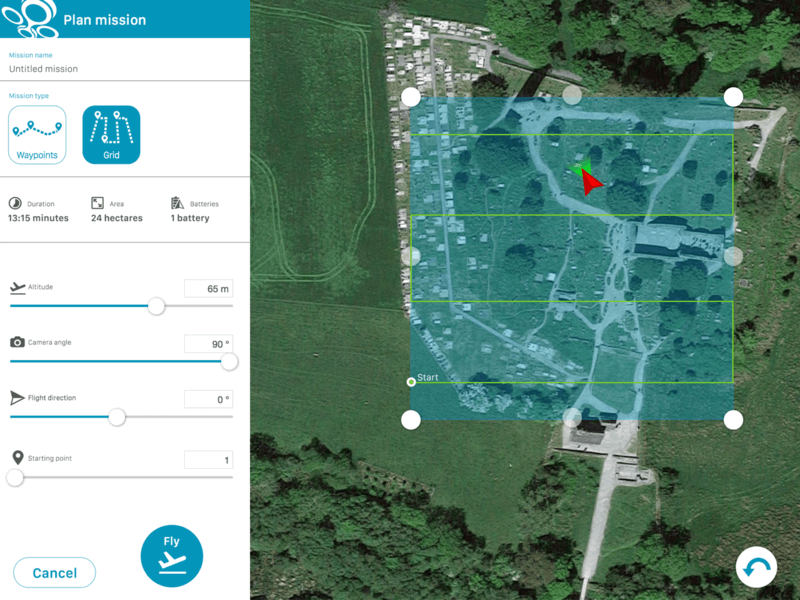
\includegraphics[scale=0.3]{figs/content_DroneSAR_screenshot_3.png}
	\caption{DroneSAR Mobile Application Showing Coverage Plan\cite{DroneSAR01}}
	\label{fig:DroneSAR}
\end{figure}

This paper also looks at coverage path planning for search and rescue, but suggests a multiple UAV approach to the problem. According to \cite{DroneSAR01}, when looking for a victim in one square kilometre on land, it takes a five-person rescue team two hours on average to find the victim. DroneSAR found that their drone could do the same job in under 20 minutes. Adding multiple UAVs to cover an area could reduce this time even more, since it would mean more area is covered per unit time. This is important because in a search and rescue operation, time is always of the essence.

This paper also focuses on a grid-based approach to the coverage problem. According to the taxonomy represented in \cite{Choset2001}, this is referred to as an approximate method. Although one can achieve complete coverage of the grid, the grid itself is not an exact representation of the environment. It does, however, greatly simplify the process of allocating areas to different UAVs, which is a key process for multiple UAV coverage. Physical implementation of this method will not be addressed as part of the scope for this paper.

% TODO: Cosider Doing The Following 
%Project description
	%Problem statement
	%Goals and Objectives
	%limitations
	%Significance of Research
	%Thesis Outline

\section{Research Aim}  
\label{sec:intro_researchAim}
The main goal of this research is to develop a coverage path planning algorithm for multiple unmanned aerial vehicles (UAVs) to search an area. The research is intended to be applicable in search and rescue operations using unmanned aerial vehicles to assist.

\section{Research Objectives}
\label{sec:intro_Objectives}
Based on the main aim of this project set out in Section \ref{sec:intro_researchAim}, a set of research objectives were formulated. These are intended to give a clearer picture of the main research goals and scope of the project. Scope and limitations are further discussed in Section \ref{sec:intro_scope} and the methodology used to achieve these objectives are detailed in Section \ref{sec:intro_method}. The research objectives are as follows:
\begin{enumerate}
	\item Develop a coverage path planning algorithm for an environment that is known a priori and contains static obstacles.
	\item Ensure that the final algorithm is an approximately complete solution.
	\item Incorporate into the algorithm's functionality an ability to have a changing number of starting UAVs that have random initial positions.
	\item Evaluate the algorithm's performance in both randomly generated and mapped, real world environments to ascertain whether or not it is suitable for search and rescue operations.
\end{enumerate}

\section{Scope and Limitations}
\label{sec:intro_scope}
%When the probability is less than 100\% for detecting a target, the advantage of a systematic search over a random or heuristic one diminishes. In demining approach. Don't need expensive sensors and such for random search. Not guaranteed to find all the targets in the area. \cite{Choset2001}
\section{System Overview}

\section{Methodology}
\label{sec:intro_method}

\section{Project Outline}
\label{sec:intro_struct}
% Later
% !TeX spellcheck = en_GB
\chapter{Literature Review}
\label{chp:LR}
As mentioned in Section \ref{sec:intro_bg}, \ac{cpp} is a subset of the general motion planning problem. This chapter will therefore begin with a brief overview of motion planning before discussing \ac{cpp} as a whole. Literature pertaining to \ac{cpp} is then discussed in several sections. Firstly, it is addressed in the context of the single robot \ac{cpp} problem. Several techniques used to achieve coverage using only one robot are summarized. 

Following this are three sections dedicated to the \ac{mcpp} problem. The first two cover distributed and non-distributed offline \ac{mcpp} respectively. This is followed by a section presenting some online \ac{mcpp} implementations. Many of the implementations were done with some application in mind, but the last section covers \acp{uav} and how they have been applied to \ac{sar} operations in particular. 
\section{Motion Planning}
\label{sec:LR-Motion Planning}
% TODO: Maybe make this section a bit shorter
One of the most noteworthy items of literature presented on motion planning is by Lavalle \cite{Lavalle2006}. In this book, a differentiation is made between motion planning and trajectory planning. Motion planning, by their definition, refers to a series of translations and/or rotations required to get an agent from one point to another within some environment. Trajectory planning would then take this plan and find a strategy to execute it within the dynamic constraints of the agent. 

\emph{Agent} is a term from the field of artificial intelligence and is interchangeable with \emph{robot} or \emph{decision maker}. The agent will be what executes the plan once it is determined. Overall, a planning algorithm is used to develop a plan for the agent to execute within an environment. Execution generally refers to a real-world implementation of a plan on some device, for example, a \ac{uav}. It can also be performed in simulation. \cite{Lavalle2006}

The type of task that is executed as well as the environment it will be executed in are important for deciding on a motion planning algorithm.  The environment may be described as discrete or continuous. Some applications, such as solving a Rubik's cube, can be represented in a discrete manner \cite{Lavalle2006}. Most robotics applications, however, are in a continuous environment, which adds a layer of complexity to problem \cite{AIbook}.

Lavalle classifies motion planning problems into discrete and continuous. He discusses point-to-point path planning algorithms such as A* and Dijkstra's Algorithm in the context of discrete path planning. He then classifies continuous problems into two major categories, namely combinatorial and sampling-based methods.

The key difference between these methods is that combinatorial methods explicitly describe the environment, including obstacles, prior to searching and guarantee completeness. Sampling-based methods are generally resolution complete or probabilistically complete, which are more lax notions of completeness. Sampling-based methods sample points in the environment and tend to perform incremental collision avoidance during pathfinding. \cite{Lavalle2006}

The notion of completeness refers to the ability of a planning algorithm to correctly find a solution if one exists, otherwise reporting that there is no solution. Resolution completeness simply guarantees completeness only down to a certain resolution, and probabilistic completeness means that the probability of reporting a correct solution converges to one. \cite{Lavalle2006}

Sampling based methods are often better at dealing with a dynamic environment, whereas combinatorial methods, also known as exact methods, require exact knowledge of the environment beforehand and cannot handle dynamic obstacles without replanning, which is very inefficient. \ac{rrt} and \ac{prm} are respective examples of single and multi-query sampling-based methods. 

Combinatorial methods utilize methods like trapezoidal decompositions and Voronoi diagrams to generate roadmaps. Roadmaps in general can easily be navigated using discrete methods like A*. \cite{Lavalle2006}

Whenever developing a plan, the task could be to move from one point to another, change orientation, or to cover every point within an environment. The task could also involve multiple agents. Optimizing paths in these scenarios can be quite challenging because agents must now not only avoid collisions with obstacles in the environment, but also with one-another, while trying to achieve a certain goal. In the context of path planning with \acp{uav}, the nature of the goal makes the problem fall into different categories, according to the authors of \cite{Zhang2020}. 

In a point-to-point problem, if the goal location is the same for all \acp{uav}, it is referred to as a rendezvous task. If they all have different goal locations, it is an allocation task. And lastly, if the goal is not to move from a starting position to a goal, but instead to cover every point in an environment, it is called a coverage task. This classification is highlighted in Figure \ref{fig:MotionPlanning}.

One final concept to grasp for motion planning, is the difference between online and offline planners. Offline algorithms draw a distinct line between the planning phase and the execution phase. The entire plan is already developed prior to real-world (or simulation based) execution, since the environment is known. Online planners tend to perform planning and execution in tandem. Generally, the environment is sensed as the agent moves and the plan is computed as it goes. The environment is either not known a priori, or is too costly to give as an input for the application. \cite{AIbook}
\begin{figure}[h!]
\centering
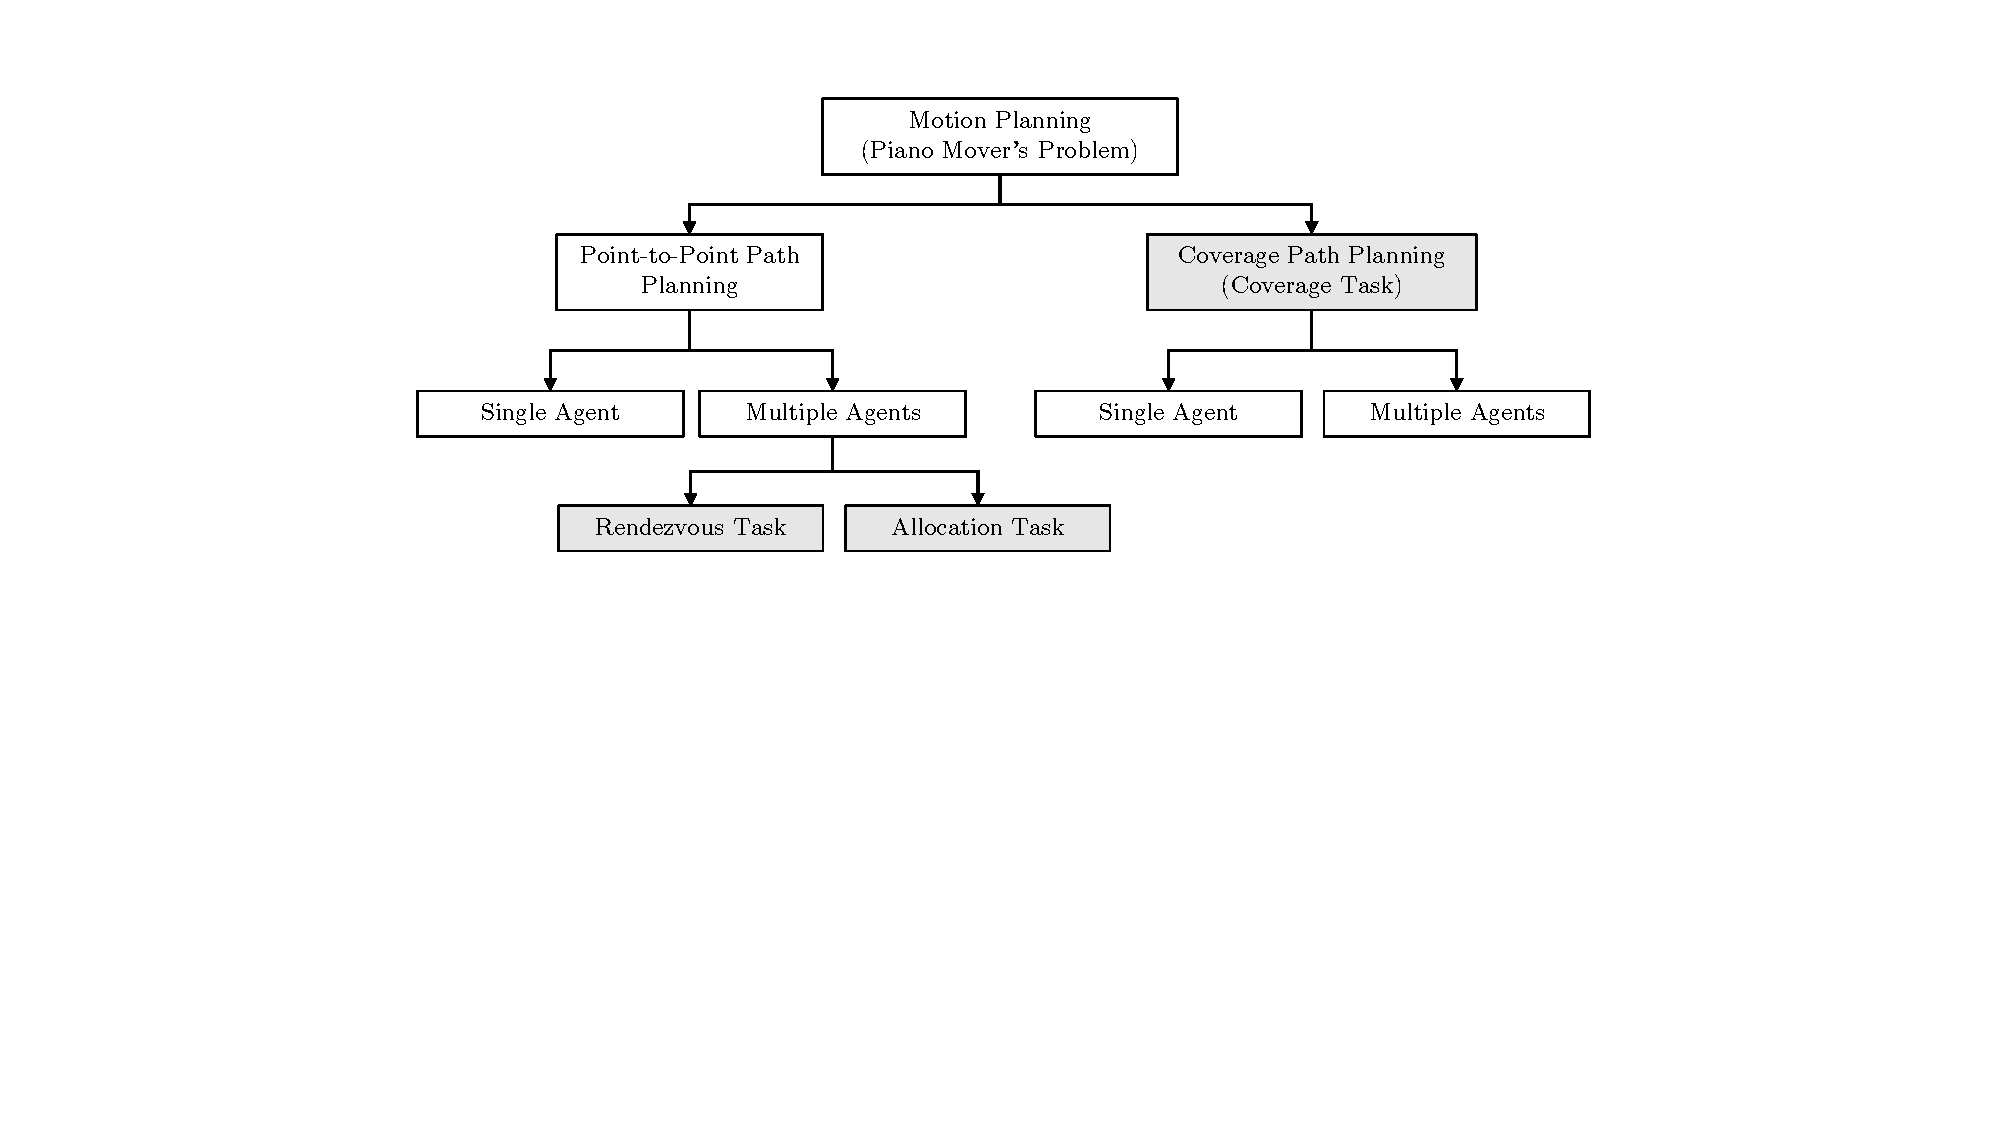
\includegraphics[width=\textwidth,trim={7cm 8.5cm 6.5cm 1.5cm},clip]{figs/Motion.pdf} % L  R
\caption{Flow diagram showing a breakdown of the different kinds of path planning as part of motion planning.}
\label{fig:MotionPlanning}
\end{figure}
\section{Coverage Path Planning}
\label{sec:LR-CPP}
% What is coverage path planning
\ac{cpp} is a subset of the general motion planning problem. The coverage task refers to visiting all points within an environment as opposed to the general start-goal type task \cite{Zhang2020}. \ac{cpp} can fall into the same categories as motion planning. It can be classified as discrete or continuous, online or offline, and as a single or multiple agent problem.

% 2001 Survey
A number of surveys have been done to give an overview of the literature available and progress made in the field of \ac{cpp}. A survey was done in 2001 wherein Choset divides \ac{cpp} into four categories \cite{Choset2001}. In later papers this is known as Choset's taxonomy, and is widely used to describe different types of \ac{cpp} algorithms.

Choset addresses heuristic and/or randomized approaches and also looks at three type of cellular decompositions, namely approximate, semi-approximate and exact. He briefly addresses the multiple robot scenario. The cellular decompositions all rely on simplifying the environment to achieve provably complete coverage. 

% TODO: STC is an approximate method. maybe reference the section that discusses that, along with other approximate methods
The approximate methods mean the environment is modelled as a set of cells with equal size and shape, generally a grid. These algorithms can achieve complete coverage of the discrete approximation of the environment, but don't guarantee complete coverage for the actual environment. Exact cellular decompositions divide the environment into polygons and cover these using simple motions e.g. back-and-forth manoeuvres. This can achieve complete coverage of the actual environment, hence the term \emph{exact}. This is further discussed in Section \ref{sec:LR - sExact}. 

% 2013 and 2019 Survey
In 2013, a survey was done regarding \ac{cpp} in robotics \cite{CPP-Survey-2013}. It expands on Choset's taxonomy and gives more detail on recent developments in each category. This paper also addresses \ac{cpp} in three-dimensional scenarios, and briefly looks at \ac{cpp} where \ac{slam} is applied due to localization uncertainties. 
% TODO: make sure you write 2D an 3D the same everywhere e.g two-dimensional
Another recent survey was published in 2019, that once again builds on Choset's taxonomy \cite{CPP-Survey-2019}. They spend more time discussing simple manoeuvres and contrast them with more complex solutions.

% 2020 Survey - multiple robots
Generally multi-robot approaches add a layer of complexity to \ac{cpp}. The most notable challenge that arises is collision avoidance. Robots need to cooperate to achieve coverage while not only avoiding collisions with obstacles, but also with each other. In 2020, a paper was compiled that specifically deals with cooperative path planning \cite{Zhang2020}. It surveys path planning with multiple \acp{uav} for the purpose of achieving many different goals, coverage being one of them.
%TODO: make sure you dont hyphenate cooperative anywhere

% TODO: Should you mention Centralized vs Decentralized (2020 paper looks at that in more detail)

% Description of offline vs online and mention that the next sections are offline, offline and online
In this chapter, a number of \ac{cpp} techniques are explored. Methods using a single robot for coverage are discussed in Section \ref{sec:LR sCPP}. Sections \ref{sec:LR Ditributed MCPP} and \ref{sec:LR Non-Distributed MCPP} refer to offline methods of \ac{mcpp} and Section \ref{sec:LR Online MCPP} looks at online methods. The sections that discuss offline methods are categorised as distributed and non-distributed.

% Definition of distributed
Distributed, for the purpose of this paper, refers to methods where the paths of individual \acp{uav} do not overlap. They are expected to fly in their own isolated sub-regions within an environment. In non-distributed methods,\acsp{uav} are free to cross paths. The area division step is not performed and so their paths are simply computed simultaneously, with knowledge of which cells have already been visited. \cite{Juan2018}

\section{Single Robot Coverage Path Planning}
\label{sec:LR sCPP}
Single robot coverage is discussed in some detail here because several of the \ac{mcpp} problems make use of them. Distributed problems tend to divide an environment into sub-regions that can then be covered using single robot techniques. Several of the other methods simply use the single robot methods and scale them to multiple robot applications. The subsections discuss a number of existing planning algorithms. This is by no means a comprehensive list of all the algorithms available, but gives a brief overview of varying techniques.%TODO: Subsection breakdown
% Mention simple maneouvres
\subsection{Exact Methods}
\label{sec:LR - sExact}
Combinatorial methods, as described by Lavalle, are also referred to as exact methods \cite{Lavalle2006}. Exact methods for \ac{cpp} make use of the same geometric principles to divide an area into cells. However, instead of creating a roadmap, an adjacency graph is created and used to move between cells. Each cell is then individually covered, generally using simple manoeuvres \cite{CPP-Survey-2013}. 

Each cell in the decomposition is a node in the adjacency graph. An exhaustive walk is used to ascertain the sequence in which to visit these nodes to achieve coverage. Simple manoeuvres, such as back-and-forth motions, are then used to cover each cell individually. These algorithms are complete, so will completely cover the environment when possible. \cite{Choset-Bous1997}

A popular method, that is mentioned in Lavalle's book, is the trapezoidal decomposition. This method decomposes an environment into trapezoids (convex cells) based on the vertices of polygonal obstacles \cite{Lavalle2006}.

The trapezoidal and boustrophedon decomposition methods are applicable in two-dimensional coverage problems. They are offline approaches, since the environment must be known a priori, and only operate with polygonal obstacles. The boustrophedon method reduces the number of cells by only looking at vertices where a line can extend both upwards and downward from it. This reduces the final length of the coverage path and makes it more efficient. \cite{CPP-Survey-2013} 
% Some simplifications of the environment are probably made to make it polygonal. The lower poly it is, the more approximate the method can become. Still more accurate than grid based though.

A more versatile exact method, that uses Morse functions for the decomposition, is also available \cite{Choset-Morse2000}. This no longer requires polygonal environments and can in theory be expanded to higher dimensional environments.

One paper sought to optimize exact cellular decomposition somewhat. This is also applied in polygonal environments. They use a greedy recursive technique to preform the decomposition and optimize the sweep direction to reduce the number of rotations. For their application, they proved that one can reduce energy consumption and the coverage route length, and thereby the time to complete coverage, by minimising rotations. \cite{Li2011}
\subsection{Sampling-Based Methods}
\label{sec:LR - sSampling}
Sampling-based methods have been adapted for coverage path planning. They are more easily scaled to three dimensional environments and are better suited to online or real-time approaches. They also deal with changing environments with dynamic obstacles more easily. \cite{Lavalle2006}

\ac{rrt} has been adapted to \ac{cpp}. An example of this is an application involving automated lawn mowing. They used \ac{rrt} as a local planner in combination with a global planner that uses a spiral motion to cover the points in a map. A solution is however, not guaranteed. Complete coverage is also not necessarily achieved because of the random nature of the paths, but it is considered a real-time approach. \cite{Nourani-Vatani2006}

Two other problems, that are both proven to be probabilistically complete, are the watchman route algorithm and the redundant roadmap algorithm \cite{Englot2012}. The watchman method constructs a roadmap, and coverage is achieved using a minimum spanning tree. The roadmap construction is done using \ac{prm} \cite{Danner2000}.% Watchmen method

The redundant roadmap method also constructs a roadmap and then conducts local point-to-point planning using \ac{rrt}, which also encompasses collision avoidance \cite{Englot2011}. 

An example of an online algorithm takes \ac{prm} and \ac{rrt} and combines them into a single point-to-point path planner, which includes dynamic replanning capabilities \cite{Wzorek2006}. These authors later expanded this to a coverage solution involving back and forth manoeuvres \cite{Rudol2008}. This is discussed in more detail in Section \ref{sec:LR SAR-Sampling}.
\subsection{A* and Wavefront Based Coverage}
\label{sec:LR - sA*}
This is a discrete method of planning. As mentioned in Section \ref{sec:LR-Motion Planning}, A* is often used in point-to-point path planning. In combinatorial motion planning or multiple-query sampling-based methods such as \ac{prm}, roadmaps are generally formed to represent the environment. These roadmaps can then be navigated using A* or another discrete algorithm like Dijkstra's algorithm or a forward search. \cite{Lavalle2006}.

A* was built from Dijkstra's algorithm, which is like a forward search that takes cost into account for the priority queue. A* is an extension of this that also predicts the cost to reach the goal using a heuristic. 

Dijkstra has also been optimised into what is called a wavefront planner. With this technique, equal cost points are grouped together into "waves" and the algorithm essentially propagates out in waves until it reaches the goal \cite{Lavalle2006}. This wavefront type planning has also been used for \ac{cpp}, with the goal to minimise rotations and the number of revisited cells \cite{Barrientos2011}.

Some authors have taken to extending A* algorithms to \ac{cpp} as well. Here the environment is generally divided into a grid and the cells can represent obstacles or free space. The starting and end-points are always within free space cells.

One of the earlier interpretations of A* \ac{cpp} is a combination of the boustrophedon method described in \ref{sec:LR - sExact} and A* \cite{Viet2012}. This is an online method that constructs boustrophedon regions incrementally and uses A* to move from one region to the next. 

In point-to-point path planning, the goal is usually to achieve the shortest path possible and the heuristic function is set up for that purpose. For \ac{cpp}, the cost function is changed to maximize coverage instead. One such implementation uses A* in a grid-based, offline approach where they try to minimise the amount of cells that get revisited \cite{Le2018}. They use critical waypoints and A* based zigzag motions. 

Another implementation uses a heuristic function with the goal of minimising the number of rotations, as was the goal of the wavefront planner mentioned earlier in this section \cite{Dogru2017}. This is useful, because rotations often consume more energy than straight line motions.
\subsection{Spanning Tree Coverage}
\label{sec: LR - sSTC}
Spanning trees are applied in discrete environments. They can be applied in offline scenarios or incrementally grown for online applications \cite{Gabriely2001}. A spanning tree is created to reach all nodes in an environment. To make a path efficient, the spanning tree is generally used on nodes that represent the centres of larger cells. 

These larger cells are then divided into four smaller cells each, which can then be the cells that are navigated by the agents. To reach each cell, the algorithm simply circumnavigates the tree. When operating in a continuous environment, the environment must be divided into the larger cells. A useful feature that this method provides is that it forms a closed loop path. The agent will always loop back to its starting point. \cite{Hazon2005} 

The spanning trees used are usually minimum spanning trees, constructed using algorithms such as Prim's algorithm. These algorithms can minimise tree weight. This weight can represent distance, or any number of other costs. They can even be used to reduce rotations by encouraging the robot to scan an area along a particular direction. \cite{Gabriely2001}

\subsection{Artificial Intelligence Methods}
\label{sec:LR - sAI}
One article compared several \ac{ai} techniques for \ac{cpp}. Four methods were compared, including one that employs a \ac{ga}. The four methods are the La Palma attraction, La Palma fuzzy logic, \ac{anfis} and \ac{pso} approaches. \cite{Juan2018}

All of the methods were implemented in a discretized environment (a grid). In this paper they also generate what they call a \emph{Risk/Occupancy Map}. This is given as an input for their algorithms to encourage searching of certain areas first. For each cell, they generate a potential risk/occupancy value ($P$). The higher the value, the higher the priority of searching that cell.

They evaluated performance of these algorithms in the context of search and rescue and found that the \ac{anfis} approach gives the best performance for that application. The attraction method works well for environments with maps that don't have a varying $P$ value. Fuzzy logic works well when a big portion of the map has high $P$ values, but has a lower success rate. \ac{pso} was shown to not work well at all.


\section{Distributed Offline MCPP}
\label{sec:LR Ditributed MCPP}
A well established offline coverage path planning approach involves the divide areas technique. This partitions an area into regions for individual robots to cover. Each robot should then be able to cover its area using one of the individual area coverage techniques mentioned in Section \ref{sec:LR sCPP}. 

The subsections are divided into different area division approaches. The methods used to perform coverage of the sub-regions are mentioned in each section seen as these are important in generating the final coverage plan. Figures are shown in these sections, all of them taken from the research papers discussed in the respective sections. These figures are purely to illustrate the different divisions that are achieved by each algorithm.
%TODO: Distributed vs Non-distributed - give the definition for the purpose of this paper
\subsection{Hexagonal Segmentation}
\label{sec:LR-Hex}
A notable distributed approach uses regular hexagons to segment the area of interest \cite{Azpurua2018}. This implementation is reminiscent of the exact methods often used for single robot coverage path planning mentioned in Section \ref{sec:LR - sExact}. Exact methods generally divide an area into arbitrarily sized polygons called cells. The robot moves between these cells and covers them using simple manoeuvres. 

In the multi-robot scenario, the area is still divided into cells, but they need to be distributed between the robots evenly for searching. The ideal situation is to assign equal sized areas to each robot so that their path lengths are similar and they can complete their paths at roughly the same time.

Hexagonal cells make it easier to assign cells to robots, seen as they are all of the same size. Hexagons are clustered using the K-means algorithm to ensure a similar number of cells are assigned to each robot. The seeds are synonymous with the robots, therefore once the seed locations are finalized for even cell distribution, the robot initial positions are established. The robots cannot start from any random location, which can be undesirable. 

The hexagons that are assigned to a given robot are contiguous and form a sub-region that is then covered using simple manoeuvres. Static obstacles are considered in this implementation, but the smallest obstacle resolution is the size of a hexagon which may not be very representative of the environment. 

Figure \ref{fig:Hex}, taken directly from their paper, illustrates the back-and-forth manoeuvres used to cover the hexagonal partitions. Black hexagons represent no-fly zones and/or static obstacles. The dark red, green and blue regions represent the sub-regions as they are assigned to the respective robots for coverage.
\begin{figure}[h!]
\centering
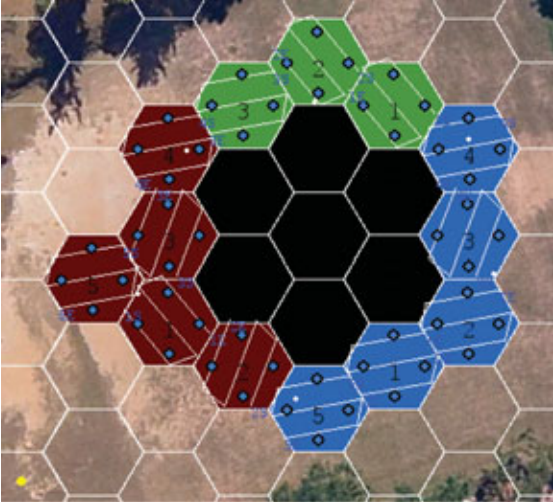
\includegraphics[scale=0.4]{figs/Hexagonal_Partitioning_Graphic}
\caption{Simulation showing coverage of hexagonal partitions with back and forth motions using three robots. \cite{Azpurua2018}}
\label{fig:Hex}
\end{figure}
\subsection{Voronoi Partitioning}
\label{sec:LR-Voronoi}
In the mathematics field, there are methods of area division to divide a polygon into a number of equal area polygons \cite{Nandakumar2012}. Another relevant method that also stems from the field of mathematics, is the Voronoi partition. This assigns regions within an area to seeds based on distance. The idea is that a region assigned to a seed represents all the points where the distance to that seed is shorter than to any other seed.\\

If the Voronoi partition is applied to the \ac{mcpp} problem, the seeds become synonymous with robots. This partition works for any number of robots at any starting positions, but unless they are evenly spaced, the areas will not have equal sizes. Distances in these scenarios are usually Euclidean and the boundaries between areas represent the position where the distances from two seeds are equal.\\ 
The authors of \cite{Nair2020} implement \ac{mcpp} using Voronoi partitions in discrete space with static obstacles. They use square discretisation of the area and compare several different methods. They investigate geodesic-Manhattan-, Manhattan-, geodesic- and Euclidean-distance-based Voronoi partitions. 

The Euclidean-based technique results in what the authors term "non-contiguous sub-regions". This means that cells that are part of a sub-region are not accessible by the robot assigned to them, due to obstacles within that sub-region. They solve this problem by using geodesic distance. This uses Euclidean measurements, but instead of a straight line distance between two cells, it calculates the distance using a collision free path between the two cells. 

Another problem arises, due to their use of discrete space. This is that when using Euclidean distances, some cells were partially in two sub-regions instead of fully in one or the other. Their solution is to use Manhattan distances. Ultimately they claim to have solved these problems by using geodesic-Manhattan-based distances to generate the partition. And thus they coined the term \ac{gm}).\\
Figure \ref{fig:Voronoi} shows figures from the paper that show the results of an area division using different distance measures with a Voronoi partition.In both figures the black blocks represent obstacles, the round dots are the robot starting positions and the black lines over the grid represent the partition boundaries. 

Figure \ref{fig:Voronoi - Euclid} shows the results using Euclidean distances. Here, the grey blocks are areas that would not be covered. This is clearly remedied using the GM-VPC technique in Figure \ref{fig:Voronoi - GM}. They implemented two different versions of \ac{gm}, which utilize respectively an exact and an approximate individual area search technique. They implemented a boustrophedon coverage plan for the exact solution and a spanning tree for the approximate version. Both of these performed better when using geodesic-Manhattan distances.   
\begin{figure}[h!]
\centering
\begin{subfigure}[b]{0.45\textwidth}
\centering
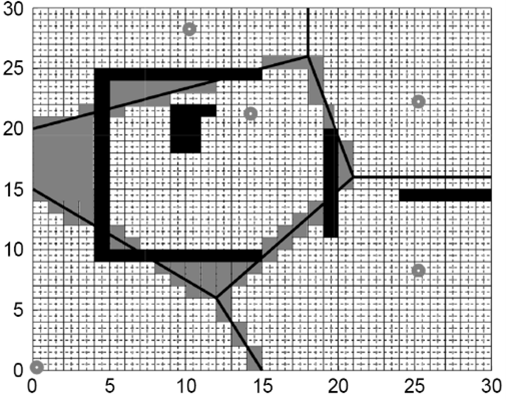
\includegraphics[scale=0.4]{figs/GM_VPC_Euclid}
\caption{Euclidean}
\label{fig:Voronoi - Euclid}
\end{subfigure}
\hfill
\begin{subfigure}[b]{0.45\textwidth}
\centering
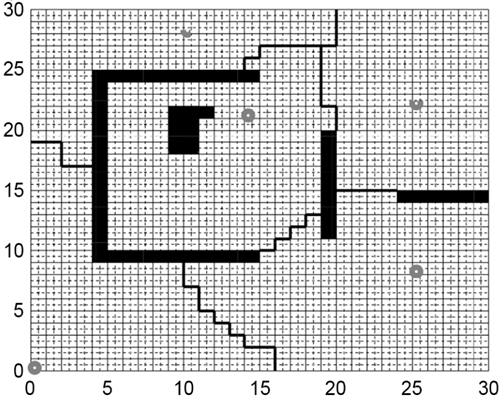
\includegraphics[scale=0.4]{figs/GM_VPC}
\caption{Geodesic-Manhattan}
\label{fig:Voronoi - GM}
\end{subfigure}
\caption{Figures showing results for the Voronoi partitioning scheme for two different distance measures. \cite{Nair2020}}
\label{fig:Voronoi}
\end{figure}
\subsection{Negotiation Protocol}
\label{sec:Negotiation}
A negotiation or bargaining protocol refers to a process involving task partitioning. In the context of area division for \ac{cpp}, the task represents the area to be divided \cite{Rossi2009}. The authors of \cite{Rossi2009} present a negotiation model based on Rubinstein's alternate-offers protocol, for the purpose of area division. The focus of their implementation was to develop a distributed algorithm capable of considering robot capabilities. This means that the robots wouldn't have to be homogeneous and can have different flight-time capabilities, manoeuvrability, on-board equipment and so forth \cite{Barrientos2011}.

They implemented their algorithm and found that it can achieve near optimum results. It tries to maximise the size of each robot's subdivision of the area (based on its capabilities), while also minimising sub-area overlap. The algorithm also works to avoid static obstacles or no fly zones that are present in the area. Moreover, they proved that it could be applied in a situation where re-planning may be necessary.

% Re-planning is necessary in a scenario when carrying out the plan changes the environment, thereby requireing replanning wiht the new environment scenario
% TODO: Future work - as new information about target becomes available - replan
A more complete implementation of the algorithm including an individual area search technique was also developed and tested \cite{Barrientos2011}. In this implementation they use a wavefront planner for the individual area coverage path generation. This requires discretisation of the area into cells. In their case, they used rectangles whose size was determined by on-board camera \ac{fov}. In order for the polygons generated by the negotiation protocol to work effectively, they use a method called Bresenham's line algorithm to approximate the lines that divide the areas in discrete space, so that they pass through the centroids of cells.

The area division achieved sometimes produces non-convex shapes, which the wavefront planner can handle effectively. Their implementation also minimizes energy consumption by minimizing the number of turns and not allowing backtracking. They also have the ability to specify the initial take-off positions of the robots. Distance from the specified take-off point to the starting point for sub-area coverage are considered in the sub-task negotiations. The authors also mention being able to specify robot landing positions pre-emptively.

One visible drawback in their implementation is that they coverage appears incomplete. The boundaries between areas pass through waypoints (cell centroids), that effectively get excluded from the coverage algorithm and are not covered. Using an exact method to search the individual areas could produce better results. Changing the boundaries to lie on the edges of cells rather than passing through their centroids could also make a difference.
\begin{figure}[h!]
\centering
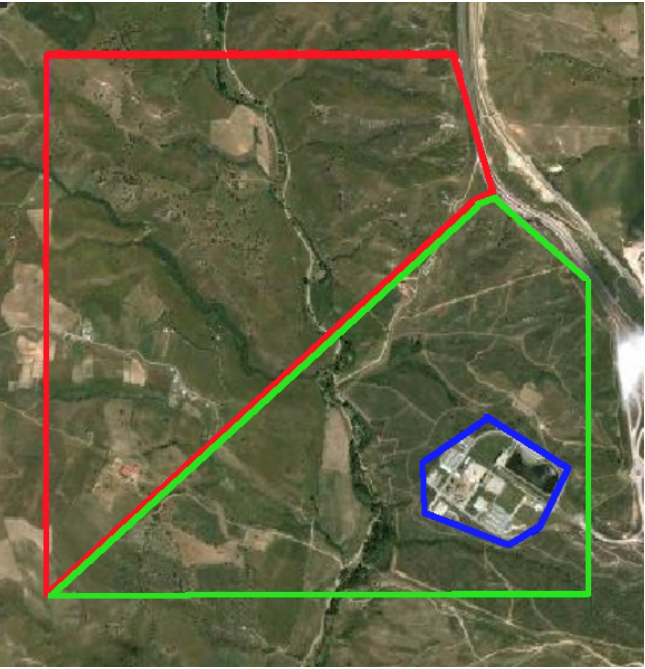
\includegraphics[scale=0.35]{figs/Negotiation_Protocol}
\caption{Figure showing the resulting area partition using the negotiation protocol. This example is for two robots and includes a no fly zone. \cite{Rossi2009}}
\label{fig:NegProt}
\end{figure}
\subsection{MSTC}
\label{sec:LR-MSTC}
\ac{mstc} is a variant of single robot \ac{stc} as presented in Section \ref{sec: LR - sSTC}. The authors of \cite{Hazon2005} designed the first variants of \ac{mstc}. The two variations they suggest are one that allows for backtracking and one that does not. Both variations still utilize a single spanning tree, but simply circumnavigate the tree with multiple robots instead of a single one.

They place a lot of emphasis on robustness and efficiency, in addition to completeness. They demonstrate an algorithm that segments the path around a spanning tree to evenly distribute it among robots. This distribution of robots is however, unrealistic. Their method becomes incredibly inefficient when robots are clustered closely together. This is because a robot simply navigates the path until it reaches the initial position of the next robot on the path.

Figure \ref{fig:MSTC} shows the paths that are generated when the robots are evenly distributed along the path that circumnavigates the tree. Blue dots represent the robot initial positions and the spanning tree is shown in red. The second method they suggest remedies this somewhat. It allows for backtracking and improves the efficiency.

The ideal situation is that all the robots have near equal path lengths, provided they are homogeneous robots. This is not guaranteed with this algorithm when the robots have random starting positions, but allowing for backtracking can improve the results and allow the coverage to be completed in a shorter amount of time.
\begin{figure}[h!]
\centering
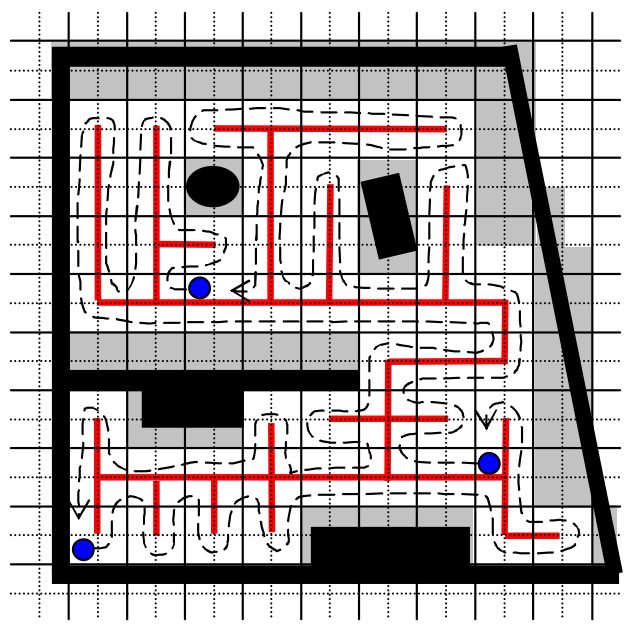
\includegraphics[scale=0.4]{figs/MSTC-Graphic}
\caption{MSTC algorithm showing the paths for three robots on an environment grid. \cite{Hazon2005}}
\label{fig:MSTC}
\end{figure}
\subsection{DARP}
\label{sec:LR DARP}
The \ac{darp} is a very interesting implementation of the distributed technique. It uses an iterative method to ensure connected sub-regions are assigned to robots, regardless of their starting positions within an environment \cite{DARP2017}.

A grid based representation of the environment is used, which includes static obstacles. Obstacles that form enclosed, unreachable spaces are not permitted. The algorithm starts by assigning cells to \acp{uav} in the environment based on which \ac{uav} is the closest to it. One cell can only be assigned to one robot.

Once this initial assignment is completed, the algorithm adjusts the distances iteratively to change assignments. The goal is to have the same number of cells assigned to each robot. This goal has the benefit of making the regions assigned to each robot the same size. By default, this means that the coverage path lengths of all the robots will be similar. The advantage of this is that the robots will finish searching at roughly the same time, making it an efficient coverage technique.

Another goal they have is to achieve connected regions. This means that the robots will not have to traverse other sub-regions, that are not assigned to them, to reach their own sub-region for searching. This once again has the benefit of improving efficiency.

The authors claim that an optimal solution is achieved if all cells are assigned to only one robot; their sub-regions are all the same size; and their sub-regions form contiguous regions. It should be noted that the connected sub-region implies that the robot's starting position is within its assigned sub-region. The results of the area subdivision achieved by DARP can be seen in Figure \ref{fig:DARP_Paper}, which is a graphic taken directly from their paper.

\begin{figure}[h!]
	\centering
	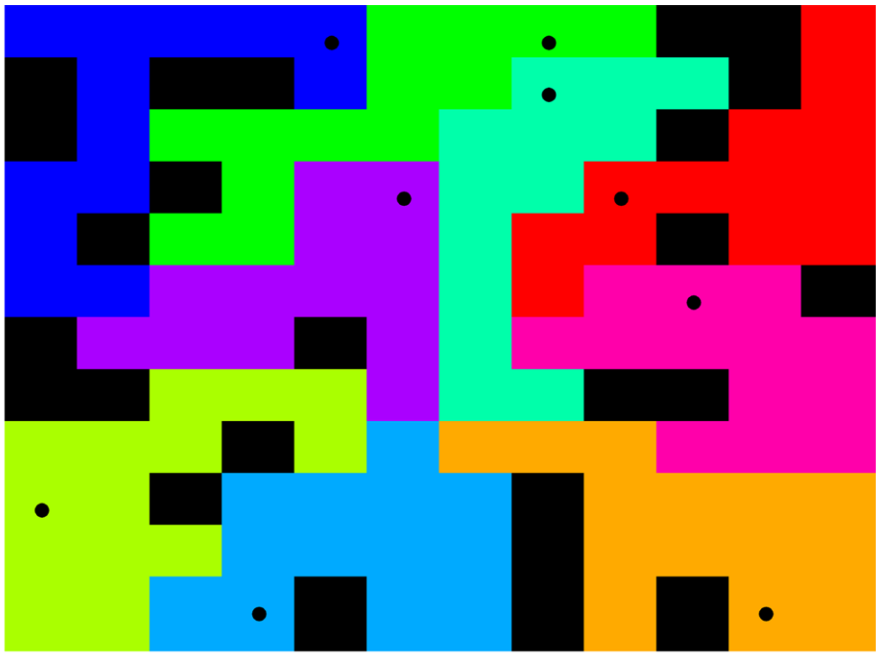
\includegraphics[scale=0.3]{figs/DARP}
	\caption{Figure showing the area division achieved on a grid with static obstacles, using DARP \cite{DARP2017}}
	\label{fig:DARP_Paper}
\end{figure}

Once these regions are computed, any grid-based individual area \ac{cpp} technique can be applied to compute coverage paths within the sub-regions. If the individual area path planners are complete, it would then mean the multi-robot path plan is complete as well.

These authors in particular decided to implement \acf{stc}, as described in Section \ref{sec: LR - sSTC}. This made the algorithm more comparable to \ac{mstc} and \ac{mfc}. These are the algorithms it sought to improve upon. They are also described respectively in Section \ref{sec:LR-MSTC} and Section \ref{sec:LR MFC}.

In the paper, a comparison is done between the algorithms to demonstrate which performs best in the sense of creating paths of equal lengths for each robot. \ac{darp} was shown to out perform both other algorithms, with at most a discrepancy of four cells between the longest and shortest paths.

Several other authors have made use of this algorithm to date. One paper uses \ac{darp} and \ac{stc}, but also adds \acl{aco} to optimize the solution even more \cite{Gao2018}. They use this to reduce the number of turns, thereby reducing overall energy consumed during flight.

Another paper takes a three-dimensional approach. Here, they are essentially addressing the unreachable region problem by allowing for vertical manoeuvres to avoid obstacles. Generally, their algorithm operates the same as the original \ac{darp} algorithm, but adds a second phase where unconnected regions are handled using three-dimensional manoeuvres. \cite{Baras2019}
\section{Non-Distributed Offline MCPP}
\label{sec:LR Non-Distributed MCPP}
This section covers methods that cannot be classified as distributed because the \acp{uav} would likely cross each others paths. The area is not divided into sub-regions as part of the planning process. These are not the type of methods that will be applied in this research paper and is therefore covered in less detail than the distributed case. The different subsections cover different techniques, as with previous sections. Interesting to note is that these methods generally build on single robot coverage techniques like those mentioned in Section \ref{sec:LR sCPP}.
\subsection{MCPP Using MFC}
\label{sec:LR MFC}
\ac{mfc} is a method that was developed by the authors in \cite{Zheng2005} to improve upon the \ac{mstc} method mentioned in Section \ref{sec:LR-MSTC}. Their intent was to construct a tree with the consideration that it will be divided afterwards, unlike what \ac{mstc} does. It allows for robot path overlap, which means there is redundant coverage and collision avoidance would need to be considered. However it can handle unique scenarios, where backtracking is unavoidable, quite well.\\ 
Their implementation is based on an algorithm presented in \cite{Even2003}. This is an approximation algorithm and they specifically looked at the rooted tree cover scenario. The roots represent the robot initial positions and then a tree is generated for each robot, using the objective to minimize the weight of the maximum weight tree. These trees are each circumnavigated by their robot (root) to cover the area.\\
Based on the simulations they ran with \ac{mstc} and \ac{mfc}, they found that \ac{mfc} generated closer to optimum results and generally achieved coverage in a shorter amount of time.	Because there is path overlap in certain scenarios, \ac{mfc} is not a truly distributed method. Results generated by this algorithm can resemble a distributed algorithm quite closely, depending on the environment.
\subsection{MCPP Using Artificial Intelligence}
\label{sec:LR-mAI}
\acl{ai} based methods have already been mentioned in Section \ref{sec:LR - sAI}. In this same paper, the application was extended to the multiple robot scenario \cite{Juan2018}. They investigate the distributed case, however they don't present their method for dividing the environment into subregions. They also investigate the free formation case for the two and three \ac{uav} scenario, and this is of more interest for the purpose of this literature review.

Free formation means that the paths for multiple \acp{uav} are planned in tandem. This means that their paths will potentially cross, implying that collision avoidance would need consideration. Distributed methods explicitly divide an area into sub-regions to be searched by individual \acp{uav}. They will never cross each other's paths, and collision avoidance is not a consideration. This paper does not address collision avoidance in the free formation case. It simply allows the paths to cross.

Three of the methods mentioned in Section \ref{sec:LR - sAI} are tested for distributed and free formation flying. \ac{pso} was not considered because it performed poorly in the single robot case. In general they found that the La Palma attraction method produces the shortest paths. The \ac{anfis} method comes in close second, and the fuzzy logic approach produces significantly longer paths. Therefore, if coverage time minimisation is important, then the attraction method performs the best.

It should be mentioned that they implemented an occupancy grid, which they generate once. This encourages the algorithms to visit certain regions of the map first. Their performance in this regard may influence one's decision to choose one algorithm over another. This will be discussed further in \ref{sec:LR-SAR-AI}, as it becomes more relevant in its particular application to \ac{sar}.
\subsection{MCPP Using Linear Programming}
Linear programming can be used to optimize linear problems with a number of variables, by trying to minimise or maximise some cost. They are also usually subject to several constraints. This methodology has been adapted to an application with multiple \acp{uav} for \ac{cpp}. \cite{Avellar2015}

The authors of this paper designed their optimization problem with the main objective of minimising coverage time. Their algorithm does this by minimising the length of the longest \ac{uav} flight path. 

One contribution they provide is the consideration of setup time. By their definition, setup time refers to the time taken by an operator to prepare a \ac{uav} for flight. They specifically consider scenarios where setup times can accumulate due to there being less operators than \acp{uav}, which leads to an accumulation of setup time for some \acp{uav}.

They apply several constraints to the problem. They limit the flight times of \acp{uav} based on battery power, set a constraint so that every node can be visited by only one \ac{uav} and limit the paths to closed-loop paths so they will always end their paths where they started. 

To ensure complete coverage they develop a constraint that ensures all nodes in one row are visited by one \ac{uav}. They also have two optional constraints to avoid diagonal lines that cross the environment. Obstacles are not considered in their implementation nor are \ac{uav} collisions. In some cases, their implementations resemble the results of a distributed case, but in some cases the algorithm still causes paths to cross.
\section{Online MCPP}
\label{sec:LR Online MCPP}
Online path planning generally refers to scenarios where a plan is generated while information about the environment is still being collected. This is often applicable in highly dynamic environments, where obstacle positions are difficult (or costly) to predict a priori. This type of planning will not be used in this project, as the environment is mapped out a priori and is not considered to by dynamic. Therefore, online planning will only be discussed briefly.

Some of the single robot coverage algorithms of Section \ref{sec:LR sCPP} have online versions. One example uses boustrophedon-A*, where the boustrophedon regions of an environment are constructed incrementally and A* is used to move from one region to the next for coverage\cite{Viet2012}. \ac{stc} can also be done online, by growing the tree incrementally \cite{Gabriely2001}. 

Sampling-based methods are well suited to online approaches. Single query approaches like \ac{rrt} avoid explicit representation of the environment and can therefore be used in dynamic environments more easily \cite{Lavalle2006}.

Often algorithms also use a hybrid of online and offline, where some information about the environment is known a priori, but data is still collected to update certain aspects of the environment incrementally. Often, because of the online element in the algorithm, overall it is still considered as an online approach. 

The paths of the \acp{uav} are generally created dynamically for online path planning, and because all the environment information cannot be known a priori, it is not possible to guarantee complete coverage.

When it comes to online \ac{cpp} with multiple robots, there are a few examples. One such example is a plan for multiple cleaning robots \cite{Luo2002}. This application implements a neural network to plan paths for multiple robots in a dynamic environment. No learning procedures were executed for this algorithm. 

The robots treat each other as dynamic obstacles within an environment and are at all times aware of the other robot positions relative to themselves. The goal is also to minimise rotations and avoid collisions with other obstacles and robots in the environment, while also covering the whole area. 

In their paper they show that the algorithm works effectively in a warehouse environment with ground vehicles, and gives real-time performance. The robots cover the entire area while avoiding collisions with each other and obstacles, and without ever crossing paths or backtracking.

An online application with multiple \acp{uav}, intended for \acl{sar} operations, was also developed. This implementation is discussed in detail in Section \ref{sec:LR SAR Decision Theory} \cite{WaharteFINAL2010}. Their algorithm iteratively updates an occupancy grid of the environment. This represents the likelihood of the target being in any given grid cell, based on the information collected. 

This information is used by each \ac{uav} to choose its next action using a steepest gradient method. This approach can arguable be considered to favour target finding over achieving coverage, but the result is similar to that of a coverage algorithm. 

Section \ref{sec:LR SAR QoS} describes another online algorithm. Here, \acs{ga} are used to optimize coverage and communication with multiple \acs{uav} in a \ac{sar} operation. Connectivity to the ground station can be prioritised to ensure new information about the target can reach the ground station efficiently. This information can be used for dynamic replanning of \ac{uav} paths. \cite{Hayat2020}

\section{UAVs and Search and Rescue}
This section covers several applications where \acp{uav} were used in \ac{sar} scenarios. These examples are not limited to the coverage scenario, and are also not limited to applications with multiple \acp{uav}. Both online and offline approaches are also mentioned. The headings in this section are designed to show the unique attributes of each implementation, which are emphasised by the respective authors in their work and add to the value of their work.
\subsection{Complete Implementation by DroneSAR}
\label{sec:LR SAR-DroneSAR}
DroneSAR is an Irish company that developed a system to assist \acl{sar} with a DJI quad-copters. The created a user-friendly application, where one can mark out an area to be searched and it will plan its own coverage path of the area. Their algorithm uses simple back and forth manoeuvres or manual user input of waypoints to plot a course. On-board video footage (visual or thermal) is sent to the ground station in real time. This allows the team on the ground to react quickly when a target is found.  \cite{DroneSAR01}

Their goal was to find a target in a \acl{sar} situation faster, and reduce risk to \ac{sar} teams on the ground. Based on tests with \acl{sar} teams, they found that the time taken to find a victim in one square kilometre, with five people searching, is roughly two hours. Their system can find the target in under 20 minutes. \cite{DroneSAR01}
 
Currently it is the job of the pilot to review footage as the drone is flying and locate a target. The drone then sends GPS coordinates to the team on the ground so they can get to the person in need. In future, they do intend to add automatic human detection algorithms using \ac{ai}. \cite{DroneSARVideo}

\subsection{Artificial Intelligence Based Approaches with Multiple UAVs}
\label{sec:LR-SAR-AI}
This method has been covered in Section \ref{sec:LR - sAI} for its application in the single robot case. It has also been addressed for multiple robots in Section \ref{sec:LR-mAI}. It should be noted that this paper was specifically developed to investigate these methods for \acl{sar} applications \cite{Juan2018}.

They developed an risk/occupancy grid for this purpose. Within the environment grid, the generate a risk/occupancy value ($P$) for each cell. The term is generated by using three different contributions.

The first of these contributions is the terrain factor ($P_{Terrain}$). This is calculated by assessing the likelihood that someone would stay within an area or enter an area and the level of danger they would be in within those areas. This factor has the biggest contribution to the final $P$-value. There is also an emergency factor ($P_{emergency}$) which represents emergency situations such as fires within an area. Lastly, there is a historical factor ($P_{historical}$) that assesses the likelihood of a historical event occurring again. This is a binary variably.

Using the $P$-values for all the cells, an risk/occupancy grid is produced that causes the algorithms to favour visiting certain cells first. This grid is not updated recursively. It is only calculated once. In Section \ref{sec:LR-mAI}, three methods are discussed and it is mentioned that the La Palma attraction approach produces the shortest times.

In a search and rescue operation, short distances are favourable because it reduces time to complete coverage. This means that a target will likely be found faster. However, this paper also has a performance measured called weight. This evaluates the algorithms' abilities to visit high $P$-value cells first. These are cells that have a high likelihood of containing the target or are high risk zones for the target to be in.

The fuzzy logic approach was found to have the lowest weights of the three methods. However, this is by such a small margin that in the end the \ac{anfis} approach seems to give the best overall performance. It has much shorter distances than the fuzzy logic approach and lower weights than the attraction approach. Therefore, the authors concluded that this approach works best for \ac{sar} in both the distributed and free formation case. 
\subsection{Online Approach with Multiple UAVs and Changing Altitudes}
\label{sec:LR SAR Decision Theory}
Several works by the same group of authors were presented regarding the use of \acp{uav} for \acl{sar} in the years 2009 and 2010. The authors published their preliminary work regarding coordinated search operations with multiple \acp{uav} \cite{Waharte2009}. 

Their setup uses quad rotors searching for a single target in a two dimensional environment. They utilise a downward facing camera as the sensing device for target detection and onboard GPS for localisation. The environment is divided into a grid and each cell is assigned a probability. This probabilistic map represents a likelihood of the target lying within each cell and forms what is called an \emph{occupancy grid}.

Updating the occupancy grid is done using a recursive Bayesian technique. The assumption of a stationary target means that all the cells are updated for every observation. The occupancy grids are calculated locally on each \ac{uav} and are only communicated to others when in communication range. This is referred to as a decoupled approach. 

Deciding on a next cell to visit is done by applying a steepest gradient method to the occupancy grid. Their simulation results show that using multiple \acp{uav}, that share information, significantly decreases the time to find the target.

In a separate paper, also by theses authors, they build on their model by including the ability to have multiple observations for one cell and account for changing altitudes of \acp{uav} \cite{Waharte2010}. Another paper addresses the actual target detection algorithm \cite{Symington2010}.

For target detection, they once again use a Bayesian estimator and evaluate the probability of target detection at changing altitudes using video data. They found that the sampling rate should be chosen according to the application. For search and rescue it should be chosen so as to minimise false negatives.

Ultimately they conclude that changing altitudes can speed up the search process. They went on to test this strategy online with three different approaches, specifically for \acl{sar} applications. The approaches were designed to deal with information sharing limitations, collision avoidance and uncertainties in the sensor data. The approach that gave the fastest target detection was the Partially Observable Markov Decision Process. \cite{WaharteFINAL2010} 

\subsection{Online Approach with One UAV and Human Detection Algorithm}
\label{sec:LR SAR-Sampling}
% Sampling-Based Methods
Sampling-based methods are good for dynamic applications. Path planning algorithms such as \ac{prm} and \ac{rrt} are well suited to online, or partially online applications. These two methods were incorporated into a single path planner as part of a navigation framework by the authors of \cite{Wzorek2006}. They also implemented dynamic replanning to account for unforeseen changes in the system. 

This can be seen as an essentially online planning algorithm because it is reactive within the environment, which is not assumed to be known in full a priori. This can be regarded as a point-to-point path planner. The navigation is is extended to \ac{cpp} in a later paper intended to be used for \ac{sar} \cite{Rudol2008}. They used their sampling-based navigation to execute back and forth motions over an area with an unmanned helicopter. The back and forth manoeuvres can be seen as a series of point-to-point navigations. 

In this paper, the main focus was however, human body detection. They collect video using a \ac{uav} with both visual and thermal cameras on-board. The footage is analysed online using an algorithm for human detection. The lower resolution thermal imagery is used to find locations of potential humans, and then higher resolution visual data is then analysed to confirm. 

According to their results, the algorithm detects humans at a rate of 25Hz. It occasionally produces false positives, but this is generally preferred over failed detections. A failure to detect a target in \acl{sar} would be catastrophic. 

% TODO: Maybe add \subsection{SAR with a Moving Target} and other SAR research 
\subsection{Multiple UAV Approach with Quality of Service Requirements}
\label{sec:LR SAR QoS}
The focus of the work by these authors is communication. A lot of emphasis was placed on getting information back to the ground station timeously. They developed a \ac{mopp} algorithm that can be tuned to favour connectivity, coverage or both in varying degrees. \cite{Hayat2020}

Coverage is important for target detection, and this is the initial goal of their algorithm. However, once a target is located, good connectivity is important to get relevant information back to the ground station as fast as possible.

Connectivity, according to the authors, is broken down into two tasks. The first task involves transmitting the location of a target back to the ground station once located. The second task is continuous monitoring of the target via a good \ac{qos} link. This sends real-time updates on the target to the ground crew.

A \acf{ga} is used to optimize the overall mission time, which includes searching the area for the target, sending the target location back to the ground crew, and establishing a good link to the ground station for continuous updates on the target. The paths found by this algorithm can be updated dynamically as new information about the target is received.

This method can be viewed as decentralized technique, because the assumption is that the \acp{uav} are not always within communication range of one another. The connectivity phase of their algorithm is used to relay information between \acp{uav} back to the ground station, which generally requires planning paths to reconfigure them for optimal connectivity. If, once the target it located, the \ac{uav} that found the target is within range of the ground station, the connectivity phase is not required.

It is interesting to see the value of incorporating connectivity as a mission goal. Their algorithms were shown to have faster mission completion times than similar algorithms that use connectivity as a constraint instead of a goal. Their results also show that favouring connectivity gives better results for a small group of \acp{uav} and favouring coverage gives better results for a larger group.


\chapter{Conceptualization and Modelling}

\section{The SAR Problem}

\section{Search Area}

\section{Environment Model}

\section{UAV Model}

\section{Collision Modelling}

\section{Target Model and Detection}
% Assume static target
% Assume the use of a visual or thermal camera
% FOV calculations
% Assume target is detected when in FOV  - either by human observers or image recognition (there might be a communications delay, but this is assumed to be negligible)
\chapter{System Overview}
\label{chp:system}

%DARP - distance measures to reduce rotations
%STC - weights to reduce rotations and / or account for weather
%Dynamic Constraints - And how it effects discretization
%Refuelling Protocol - The initial stages of an algorithm that provides for refuelling

%Simulation of SAR
%\begin{landscape}
\begin{figure}[h!]
	\centering
	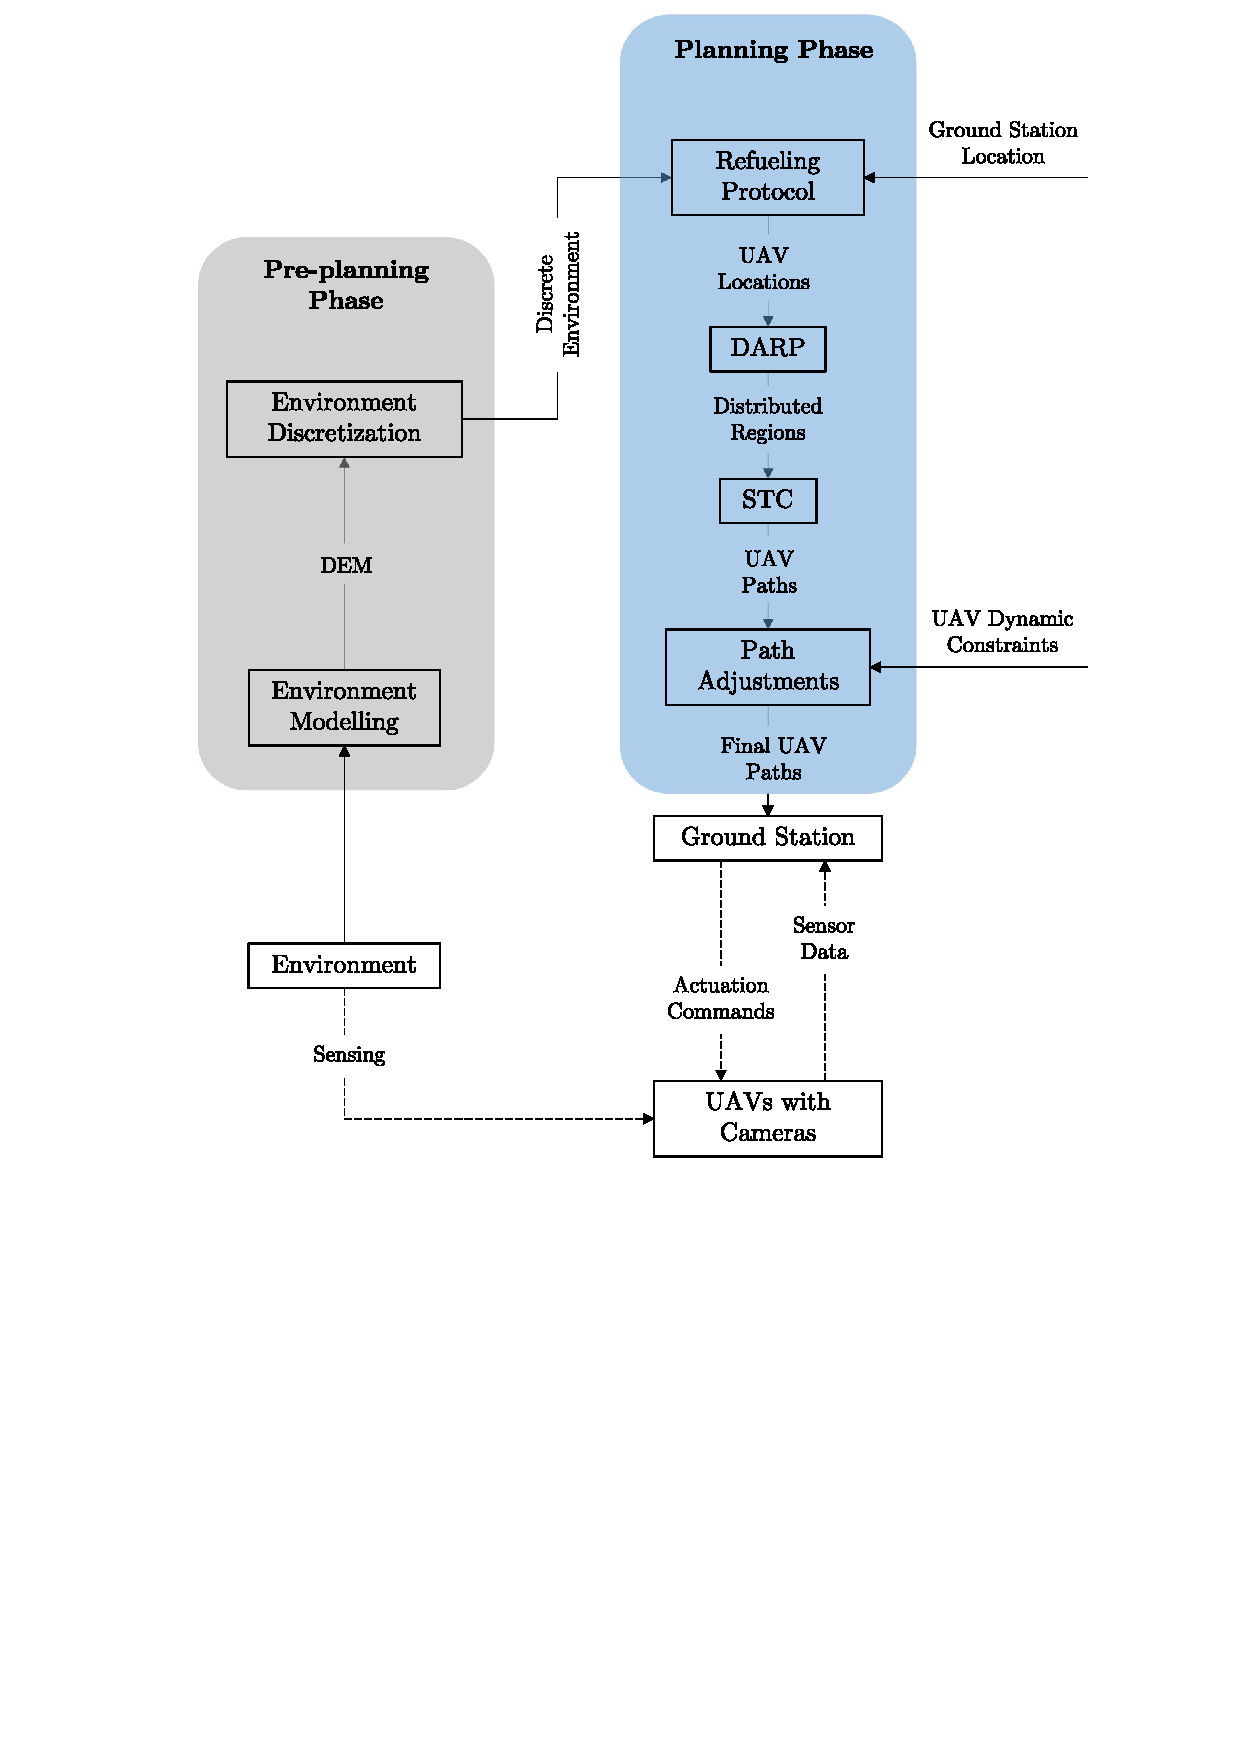
\includegraphics[width=\textwidth,trim={3cm 8.5cm 2.5cm 0cm},clip]{figs/SOD.pdf}
	\caption{Diagram showing an overview of the multi-robot SAR system.}
	\label{fig:SOD}
\end{figure}
%\end{landscape}

\chapter{Environment Representation}
\label{chp:ER}
\acresetall
This Chapter describes the thought process behind the environment representation. Section \ref{sec:ER-bg} gives relevant background information and context for the problem, and Section \ref{sec:ER-ED} describes how this information is used to formulate a discrete environment representation. Lastly, Section \ref{sec:ER-App} shows a few practical scenarios using this strategy with different on-board cameras. 

\section{Background}
\label{sec:ER-bg}
\subsection{Assumptions}
The goal of this paper is to develop a coverage path planning algorithm \hbox{applicable} in a \ac{sar} situation, using \acp{uav}. To achieve success in such an application, the first step would be to find a way to represent the environment. Essentially, the context in which the \acp{uav} exist needs to be described in some way for them to navigate it successfully.
 
% Offline
The starting assumption is that an offline approach is sufficient. This implies that there is always enough information known about the environment to represent it fully prior to the execution of the path planning algorithm. At the altitude that a \ac{uav} flies, it is reasonable to assume that any obstructions, for example power lines or mountains, can be mapped out a priori. Moreover, \ac{sar} operations often have fixed geographical bounds in which to search.

% No dynamic obstacles or moving target
% TODO: Justify why the target is not assumed to be in motion
Furthermore, it is also assumed that there are no transients in the environment, such as a moving target or dynamic obstacles. Search and rescue operations will rarely have moving elements at the altitude of the \acp{uav}. They are more likely to have fixed no fly zones and static obstacles.

% Two dimensional
Because they are airborne vehicles,\acp{uav} can execute three dimensional movements, which implies the necessity for a three dimensional representation of the environment. In this paper however, it is assumed that altitude changes are not necessary to search an area. Assuming that there is some form of camera on-board the \ac{uav}, a constant altitude will be an advantage. It means that the \ac{gsd} will remain roughly constant, which is a widely accepted measure of camera accuracy. Assuming a camera is on a \ac{uav} pointing down towards the ground, \ac{gsd} is the distance on the ground as represented by the width of one pixel in an image \cite{PropellerAero2021}.

Without altitude changes, \ac{uav} motions can be represented in two-dimensional space, which greatly simplifies the problem. For offline coverage path planning, it is important to have some demarcated two-dimensional region that requires coverage. The identified region, or environment, can be represented in either a discrete or continuous manner. 

% Discrete
% TODO: Mention drawbacks of continuous implementations
% TODO: Mention reasons for choosing discrete - wavefront planner paper pg 674 "An exact cell decomposition is ineffiecient because we are interested in acquiring an equally sized set of images"
In the context of \ac{sar}, complete coverage is very important. It will ensure that every possible point in the environment map is covered. In this scenario, it implies that the camera will have viewed all points on the map. Achieving completeness is by no means trivial, but is more achievable in complex environments when using a discrete approach.

\subsection{Discretisation Using Cameras}
Discretising the environment can be done in a few different ways. Assuming a generic \ac{uav} with some thermal or visual camera on-board, one has a few options. One can discretise the area based on the \ac{uav} size, but a more common practice is to base it off the tool size. In this case, that would be the \ac{fov} of the on-board camera. This also makes the process of complete coverage easier, because if the camera is guaranteed to see the entirety of each discrete cell, it is a complete algorithm so long as each cell is visited.

Therefore, to discretise the environment, the \ac{fov} needs to be calculated. The camera specifications and \ac{uav} altitude will be the determining factors to calculate the \ac{fov}. The type of camera and the flight altitude are design decisions and will depend on the \ac{gsd} necessary to realistically be able to locate the target in a \ac{sar} operation.

The diagram in Figure \ref{fig:FOV} shows all the relevant variables needed to calculate the \acl{fov} along one dimension ($FOV_x$). A similar diagram can be used to calculate the \acl{fov} along the other dimension ($FOV_y$). The only difference would be the sensor size variable, which changes from the sensor width ($w_{len}$) to the sensor height ($h_{len}$). The other variables include the focal length of the camera ($f$), the height of the lens above ground ($H$) and the camera's angle of view ($AOV$). Lastly, there is the variable $\phi$ which is an angle created due to the sensor being slightly smaller than the diameter of the cone of light projected onto it.

The resulting \acl{fov} will be a rectangle of the same aspect ratio of the camera sensor, provided the camera is pointing directly down and the ground is level. For this application, it is assumed the camera is always pointing downwards. This can be accomplished when the \acs{uav} banks by placing the camera on a gimble. The assumption that the ground is level is not entirely reasonable, for example, in a mountainous region. This can be addressed by adding overlap between images to add some redundant coverage, which will be added in Chapter \ref{chp:refuelling}. Doing a topographical inspection is beyond the scope of this project and will not be addressed in more detail.
% TODO: Check this reference and decide whether to include last sentence
\tikzset{every picture/.style={line width=0.75pt}} %set default line width to 0.75pt          
\begin{figure}[h!]
	\centering	      
	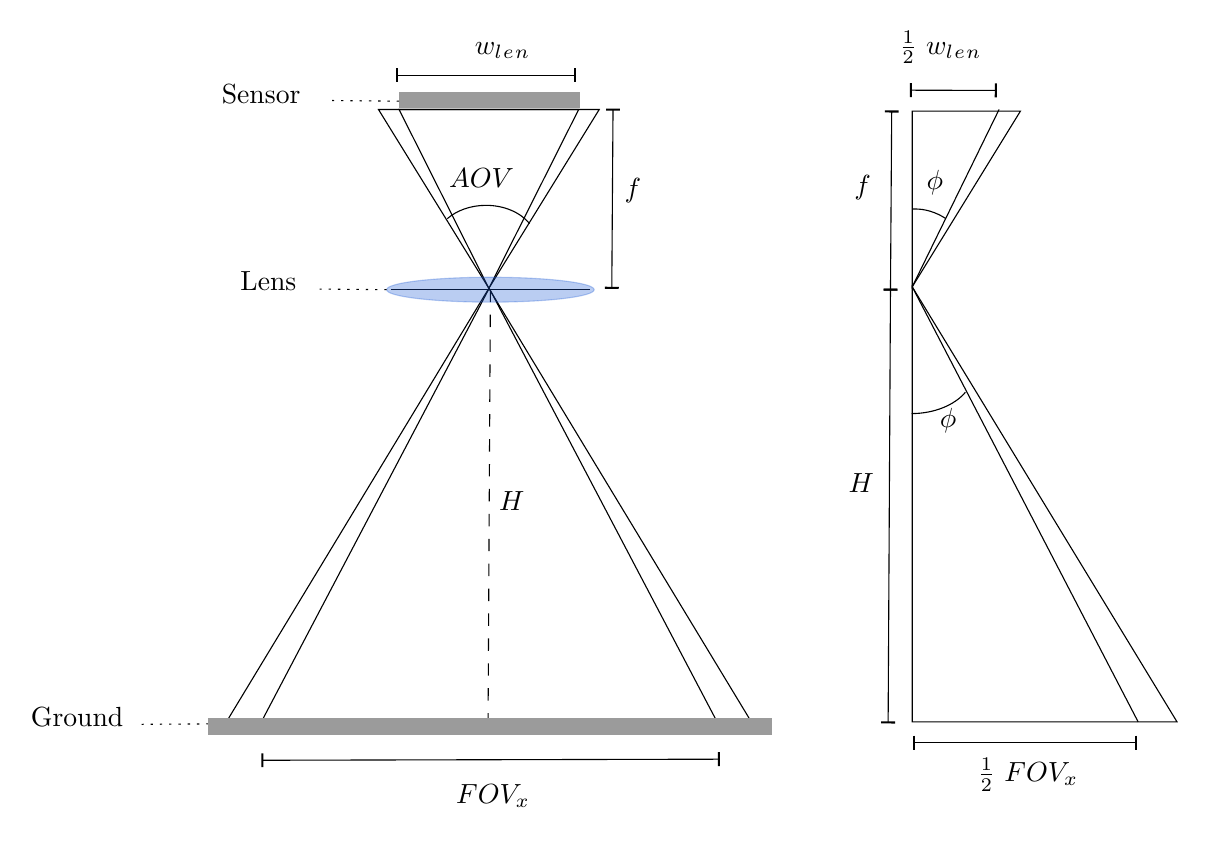
\begin{tikzpicture}[x=0.75pt,y=0.75pt,yscale=-1,xscale=1]
		%uncomment if require: \path (0,445); %set diagram left start at 0, and has height of 445
		
		%Shape: Triangle [id:dp7279031821934365] 
		\draw   (292.52,162.29) -- (239.35,76.17) -- (345.69,76.17) -- cycle ;
		%Shape: Triangle [id:dp08500924272014787] 
		\draw   (292.52,162.29) -- (419.57,372.17) -- (165.48,372.17) -- cycle ;
		%Straight Lines [id:da9387157545116658] 
		\draw    (245.26,162.97) -- (341.26,162.97) ;
		%Shape: Triangle [id:dp15441481766796317] 
		\draw   (292.52,162.29) -- (249.26,76.17) -- (335.78,76.17) -- cycle ;
		%Shape: Triangle [id:dp8187279481172025] 
		\draw   (292.69,162.29) -- (403,372.17) -- (182.39,372.17) -- cycle ;
		%Straight Lines [id:da06491692932377724] 
		\draw    (248.39,59.69) -- (334.14,59.69) ;
		\draw [shift={(334.14,59.69)}, rotate = 180] [color={rgb, 255:red, 0; green, 0; blue, 0 }  ][line width=0.75]    (0,3.35) -- (0,-3.35)   ;
		\draw [shift={(248.39,59.69)}, rotate = 180] [color={rgb, 255:red, 0; green, 0; blue, 0 }  ][line width=0.75]    (0,3.35) -- (0,-3.35)   ;
		%Straight Lines [id:da8254572040663344] 
		\draw    (352.34,76.22) -- (351.75,162.07) ;
		\draw [shift={(351.75,162.07)}, rotate = 270.39] [color={rgb, 255:red, 0; green, 0; blue, 0 }  ][line width=0.75]    (0,3.35) -- (0,-3.35)   ;
		\draw [shift={(352.34,76.22)}, rotate = 270.39] [color={rgb, 255:red, 0; green, 0; blue, 0 }  ][line width=0.75]    (0,3.35) -- (0,-3.35)   ;
		%Straight Lines [id:da18153445552160163] 
		\draw  [dash pattern={on 4.5pt off 4.5pt}]  (293.26,162.97) -- (292.13,371.48) ;
		%Shape: Right Triangle [id:dp9464990257102419] 
		\draw   (548.64,76.92) -- (496.5,161.6) -- (496.5,76.94) -- cycle ;
		%Straight Lines [id:da9593228177444686] 
		\draw    (496.5,161.6) -- (538.33,76.17) ;
		%Shape: Arc [id:dp3427993390498929] 
		\draw  [draw opacity=0] (496.65,124.11) .. controls (496.93,124.1) and (497.22,124.09) .. (497.5,124.09) .. controls (502.76,124) and (507.83,125.61) .. (512.56,128.62) -- (498.77,204.83) -- cycle ; \draw   (496.65,124.11) .. controls (496.93,124.1) and (497.22,124.09) .. (497.5,124.09) .. controls (502.76,124) and (507.83,125.61) .. (512.56,128.62) ;
		%Straight Lines [id:da5534147172451449] 
		\draw    (495.86,66.85) -- (536.76,66.97) ;
		\draw [shift={(536.76,66.97)}, rotate = 180.17] [color={rgb, 255:red, 0; green, 0; blue, 0 }  ][line width=0.75]    (0,3.35) -- (0,-3.35)   ;
		\draw [shift={(495.86,66.85)}, rotate = 180.17] [color={rgb, 255:red, 0; green, 0; blue, 0 }  ][line width=0.75]    (0,3.35) -- (0,-3.35)   ;
		%Straight Lines [id:da49349314045709525] 
		\draw    (486.61,77.11) -- (486.02,162.96) ;
		\draw [shift={(486.02,162.96)}, rotate = 270.39] [color={rgb, 255:red, 0; green, 0; blue, 0 }  ][line width=0.75]    (0,3.35) -- (0,-3.35)   ;
		\draw [shift={(486.61,77.11)}, rotate = 270.39] [color={rgb, 255:red, 0; green, 0; blue, 0 }  ][line width=0.75]    (0,3.35) -- (0,-3.35)   ;
		%Shape: Arc [id:dp09088039941092019] 
		\draw  [draw opacity=0] (272.52,128.74) .. controls (277.02,124.82) and (283.7,122.33) .. (291.17,122.33) .. controls (300.03,122.33) and (307.8,125.84) .. (312.1,131.09) -- (291.17,140.58) -- cycle ; \draw   (272.52,128.74) .. controls (277.02,124.82) and (283.7,122.33) .. (291.17,122.33) .. controls (300.03,122.33) and (307.8,125.84) .. (312.1,131.09) ;
		%Shape: Right Triangle [id:dp9191394953697831] 
		\draw   (496.5,161.6) -- (624.06,371.17) -- (496.5,371.17) -- cycle ;
		%Straight Lines [id:da9606752421348479] 
		\draw    (605.33,371.17) -- (496.5,161.6) ;
		%Shape: Arc [id:dp6813474716985082] 
		\draw  [draw opacity=0] (522.1,212.41) .. controls (516.97,218.5) and (507.3,222.62) .. (496.19,222.67) -- (496,202.42) -- cycle ; \draw   (522.1,212.41) .. controls (516.97,218.5) and (507.3,222.62) .. (496.19,222.67) ;
		%Straight Lines [id:da806740169220673] 
		\draw    (183.39,389.69) -- (403.33,389.17) ;
		\draw [shift={(403.33,389.17)}, rotate = 539.86] [color={rgb, 255:red, 0; green, 0; blue, 0 }  ][line width=0.75]    (0,3.35) -- (0,-3.35)   ;
		\draw [shift={(183.39,389.69)}, rotate = 539.86] [color={rgb, 255:red, 0; green, 0; blue, 0 }  ][line width=0.75]    (0,3.35) -- (0,-3.35)   ;
		%Straight Lines [id:da8133225602503578] 
		\draw    (497.33,381.17) -- (604.33,381.17) ;
		\draw [shift={(604.33,381.17)}, rotate = 180] [color={rgb, 255:red, 0; green, 0; blue, 0 }  ][line width=0.75]    (0,3.35) -- (0,-3.35)   ;
		\draw [shift={(497.33,381.17)}, rotate = 180] [color={rgb, 255:red, 0; green, 0; blue, 0 }  ][line width=0.75]    (0,3.35) -- (0,-3.35)   ;
		%Straight Lines [id:da25053349814928394] 
		\draw    (486.02,162.96) -- (484.89,371.47) ;
		\draw [shift={(484.89,371.47)}, rotate = 270.31] [color={rgb, 255:red, 0; green, 0; blue, 0 }  ][line width=0.75]    (0,3.35) -- (0,-3.35)   ;
		\draw [shift={(486.02,162.96)}, rotate = 270.31] [color={rgb, 255:red, 0; green, 0; blue, 0 }  ][line width=0.75]    (0,3.35) -- (0,-3.35)   ;
		%Shape: Rectangle [id:dp5196090784877698] 
		\draw  [color={rgb, 255:red, 155; green, 155; blue, 155 }  ,draw opacity=1 ][fill={rgb, 255:red, 155; green, 155; blue, 155 }  ,fill opacity=1 ] (249.26,68.14) -- (336,68.14) -- (336,75.17) -- (249.26,75.17) -- cycle ;
		%Shape: Ellipse [id:dp39537204861922115] 
		\draw  [color={rgb, 255:red, 26; green, 88; blue, 211 }  ,draw opacity=0.3 ][fill={rgb, 255:red, 26; green, 88; blue, 211 }  ,fill opacity=0.3 ] (243.26,162.97) .. controls (243.26,159.66) and (265.64,156.97) .. (293.26,156.97) .. controls (320.87,156.97) and (343.26,159.66) .. (343.26,162.97) .. controls (343.26,166.29) and (320.87,168.97) .. (293.26,168.97) .. controls (265.64,168.97) and (243.26,166.29) .. (243.26,162.97) -- cycle ;
		%Shape: Boxed Line [id:dp7067135001640237] 
		\draw  [dash pattern={on 0.84pt off 2.51pt}]  (243.26,162.97) -- (211,162.67) ;
		%Straight Lines [id:da962687715126145] 
		\draw  [dash pattern={on 0.84pt off 2.51pt}]  (157.48,372.17) -- (125.22,372.37) ;
		%Shape: Boxed Line [id:dp25644897900816477] 
		\draw  [dash pattern={on 0.84pt off 2.51pt}]  (249.26,72.14) -- (217,71.84) ;
		%Straight Lines [id:da9121328450253205] 
		\draw [color={rgb, 255:red, 155; green, 155; blue, 155 }  ,draw opacity=1 ][line width=6]    (157.17,373.35) -- (429.09,373.35) ;
		
		% Text Node
		\draw (277.85,37.29) node [anchor=north west][inner sep=0.75pt]  [font=\normalsize]  {$ \begin{array}{l}
				w_{l}{}_{e}{}_{n}\\
			\end{array}$};
		% Text Node
		\draw (171.59,152.9) node [anchor=north west][inner sep=0.75pt]  [font=\normalsize] [align=left] {Lens};
		% Text Node
		\draw (356.67,108.27) node [anchor=north west][inner sep=0.75pt]  [font=\normalsize]  {$f$};
		% Text Node
		\draw (296.25,259.08) node [anchor=north west][inner sep=0.75pt]  [font=\normalsize]  {$H$};
		% Text Node
		\draw (272.06,103.36) node [anchor=north west][inner sep=0.75pt]  [font=\normalsize]  {$AOV$};
		% Text Node
		\draw (502.19,104.3) node [anchor=north west][inner sep=0.75pt]  [font=\normalsize]  {$\phi $};
		% Text Node
		\draw (467.33,106.6) node [anchor=north west][inner sep=0.75pt]  [font=\normalsize]  {$f$};
		% Text Node
		\draw (489,37) node [anchor=north west][inner sep=0.75pt]    {$\frac{1}{2} \ w_{l}{}_{e}{}_{n}$};
		% Text Node
		\draw (508.52,218.96) node [anchor=north west][inner sep=0.75pt]  [font=\normalsize]  {$\phi $};
		% Text Node
		\draw (268.85,398.07) node [anchor=north west][inner sep=0.75pt]  [font=\normalsize]  {$ \begin{array}{l}
				FOV_{x}\\
			\end{array}$};
		% Text Node
		\draw (520,387.4) node [anchor=north west][inner sep=0.75pt]  [font=\normalsize]  {$ \begin{array}{l}
				\frac{1}{2} \ FOV_{x}\\
			\end{array}$};
		% Text Node
		\draw (464.59,250.41) node [anchor=north west][inner sep=0.75pt]  [font=\normalsize]  {$H$};
		% Text Node
		\draw (162.59,62.9) node [anchor=north west][inner sep=0.75pt]  [font=\normalsize] [align=left] {Sensor};
		% Text Node
		\draw (70.59,363) node [anchor=north west][inner sep=0.75pt]  [font=\normalsize] [align=left] {Ground};
		
		
	\end{tikzpicture}
	\caption{Diagram showing relevant variables concerned with calculating the Field of View for a camera.}
	\label{fig:FOV}
\end{figure}
The calculations required to do a discretisation based on the camera \ac{fov} will now be discussed. The first equation that is required is the calculation of the angle $\phi$ which makes use of the small triangle:
\begin{equation}
	\label{eqn:phi}
	\begin{aligned}
		\tan{\phi} &= \frac{\frac{1}{2}w_{len}}{f} &\\
		\phi &= \tan^{-1}{(\frac{w_{len}}{2f})}
	\end{aligned}	
\end{equation}
Now that $\phi$ is known, the bigger triangle is used to calculate $FOV_x$:
\begin{equation}
	\label{eqn:fov_x}
	\begin{aligned}
		\frac{FOV_x}{2} &= H \times \tan{\phi} &\\
		FOV_x &= 2H \times \tan{ (\tan^{-1}{ (\frac{w_{len}}{2f}) }) } &\\
		FOV_x &= H \times \frac{w_{len}}{f} &\\
	\end{aligned}
\end{equation}
Similarly, $FOV_y$ can be calculated using the other sensor size dimension $h_{len}$:
\begin{equation}
	\label{eqn:fov_y}
	\begin{aligned}
		FOV_y &= H \times \frac{h_{len}}{f}
	\end{aligned}
\end{equation}
Both $FOV_x$ and $FOV_y$ will have the same units as $H$, which is metres. The resolution of the camera is the number of pixels along the image width ($px_w$) multiplied with the number of pixels along its height ($px_h$). These can be used to calculate the $GSD$ by dividing either $FOV$ by the pixel value associated with that dimension:
\begin{equation}
	\label{eqn:GSD}
	\begin{aligned}
		GSD &= \frac{100FOV_x}{px_w} &\\
		GSD &= \frac{100H \times w_{len}}{f \times px_w}
	\end{aligned}
\end{equation}

\section{Discretisation Methodology}
\label{sec:ER-ED}
If the size of the environment discretisation is set equal to the rectangular camera field of view, and the type of camera used is known, then a desired $GSD$ can be used to decide on an appropriate flying height. Choosing a $GSD$ would depend on the application, seen as it represents the level of detail that can potentially be detected in an image.\\
Taking the conservative approach, the assumption is that one is looking for a human being standing upright, viewed from above. To get a good estimate of the space occupied by a human in this orientation, one needs anthropometric data. A survey was done in Europe for people between the ages of 18 and 60 \cite{Jurgens1998}. Among other measurements, they measured chest depth ($w$) and elbow-to-elbow length ($l$). These dimensions represent those of an upright human from above and can be seen in Figure \ref{fig:GSD}.\\ 
\tikzset{every picture/.style={line width=0.75pt}} %set default line width to 0.75pt        
\begin{figure}
	\centering
	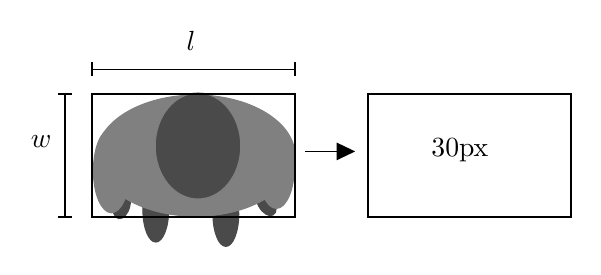
\begin{tikzpicture}[x=0.75pt,y=0.75pt,yscale=-1,xscale=1]
		%uncomment if require: \path (0,300); %set diagram left start at 0, and has height of 300
		
		%Shape: Ellipse [id:dp5061908839346234] 
		\draw  [color={rgb, 255:red, 74; green, 74; blue, 74 }  ,draw opacity=1 ][fill={rgb, 255:red, 74; green, 74; blue, 74 }  ,fill opacity=1 ] (394.62,193.23) .. controls (392.81,189.9) and (392.91,186.34) .. (394.85,185.28) .. controls (396.79,184.23) and (399.83,186.07) .. (401.65,189.41) .. controls (403.47,192.74) and (403.37,196.3) .. (401.43,197.36) .. controls (399.49,198.41) and (396.44,196.57) .. (394.62,193.23) -- cycle ;
		%Shape: Ellipse [id:dp4772697686098053] 
		\draw  [color={rgb, 255:red, 74; green, 74; blue, 74 }  ,draw opacity=1 ][fill={rgb, 255:red, 74; green, 74; blue, 74 }  ,fill opacity=1 ] (324.6,191.47) .. controls (325.46,187.77) and (327.9,185.18) .. (330.05,185.68) .. controls (332.2,186.18) and (333.25,189.58) .. (332.4,193.28) .. controls (331.54,196.98) and (329.1,199.57) .. (326.95,199.07) .. controls (324.8,198.57) and (323.75,195.17) .. (324.6,191.47) -- cycle ;
		%Shape: Ellipse [id:dp7464833674207887] 
		\draw  [color={rgb, 255:red, 74; green, 74; blue, 74 }  ,draw opacity=1 ][fill={rgb, 255:red, 74; green, 74; blue, 74 }  ,fill opacity=1 ] (372.5,196.92) .. controls (372.5,188.32) and (375.28,181.35) .. (378.71,181.35) .. controls (382.13,181.35) and (384.91,188.32) .. (384.91,196.92) .. controls (384.91,205.53) and (382.13,212.5) .. (378.71,212.5) .. controls (375.28,212.5) and (372.5,205.53) .. (372.5,196.92) -- cycle ;
		%Shape: Ellipse [id:dp9681716059666354] 
		\draw  [color={rgb, 255:red, 74; green, 74; blue, 74 }  ,draw opacity=1 ][fill={rgb, 255:red, 74; green, 74; blue, 74 }  ,fill opacity=1 ] (338.74,194.85) .. controls (338.74,186.24) and (341.52,179.27) .. (344.95,179.27) .. controls (348.37,179.27) and (351.15,186.24) .. (351.15,194.85) .. controls (351.15,203.45) and (348.37,210.42) .. (344.95,210.42) .. controls (341.52,210.42) and (338.74,203.45) .. (338.74,194.85) -- cycle ;
		%Shape: Ellipse [id:dp7224271801321214] 
		\draw  [color={rgb, 255:red, 128; green, 128; blue, 128 }  ,draw opacity=1 ][fill={rgb, 255:red, 128; green, 128; blue, 128 }  ,fill opacity=1 ] (316.38,168.78) .. controls (316.38,152.66) and (337.79,139.6) .. (364.19,139.6) .. controls (390.59,139.6) and (412,152.66) .. (412,168.78) .. controls (412,184.9) and (390.59,197.96) .. (364.19,197.96) .. controls (337.79,197.96) and (316.38,184.9) .. (316.38,168.78) -- cycle ;
		%Shape: Ellipse [id:dp3950279689736771] 
		\draw  [color={rgb, 255:red, 128; green, 128; blue, 128 }  ,draw opacity=1 ][fill={rgb, 255:red, 74; green, 74; blue, 74 }  ,fill opacity=1 ] (365.29,138.6) .. controls (376.67,138.6) and (385.9,150.04) .. (385.9,164.15) .. controls (385.9,178.25) and (376.67,189.69) .. (365.29,189.69) .. controls (353.9,189.69) and (344.67,178.25) .. (344.67,164.15) .. controls (344.67,150.04) and (353.9,138.6) .. (365.29,138.6) -- cycle ;
		%Shape: Ellipse [id:dp14441581895383182] 
		\draw  [color={rgb, 255:red, 128; green, 128; blue, 128 }  ,draw opacity=1 ][fill={rgb, 255:red, 128; green, 128; blue, 128 }  ,fill opacity=1 ] (314.91,176.05) .. controls (314.91,164.87) and (318.8,155.8) .. (323.6,155.8) .. controls (328.4,155.8) and (332.29,164.87) .. (332.29,176.05) .. controls (332.29,187.23) and (328.4,196.3) .. (323.6,196.3) .. controls (318.8,196.3) and (314.91,187.23) .. (314.91,176.05) -- cycle ;
		%Shape: Ellipse [id:dp8509174208950578] 
		\draw  [color={rgb, 255:red, 128; green, 128; blue, 128 }  ,draw opacity=1 ][fill={rgb, 255:red, 128; green, 128; blue, 128 }  ,fill opacity=1 ] (394.35,173.97) .. controls (394.35,162.79) and (398.24,153.72) .. (403.03,153.72) .. controls (407.83,153.72) and (411.72,162.79) .. (411.72,173.97) .. controls (411.72,185.16) and (407.83,194.22) .. (403.03,194.22) .. controls (398.24,194.22) and (394.35,185.16) .. (394.35,173.97) -- cycle ;
		%Shape: Rectangle [id:dp6763821992887933] 
		\draw  [line width=0.75]  (314.19,139.1) -- (412.19,139.1) -- (412.19,198.46) -- (314.19,198.46) -- cycle ;
		%Straight Lines [id:da0050447787628182805] 
		\draw    (314.19,127.1) -- (412.19,127.1) ;
		\draw [shift={(412.19,127.1)}, rotate = 180] [color={rgb, 255:red, 0; green, 0; blue, 0 }  ][line width=0.75]    (0,3.35) -- (0,-3.35)   ;
		\draw [shift={(314.19,127.1)}, rotate = 180] [color={rgb, 255:red, 0; green, 0; blue, 0 }  ][line width=0.75]    (0,3.35) -- (0,-3.35)   ;
		%Shape: Rectangle [id:dp8520376009638861] 
		\draw  [line width=0.75]  (447.19,139.1) -- (545.19,139.1) -- (545.19,198.46) -- (447.19,198.46) -- cycle ;
		%Straight Lines [id:da004734927691815605] 
		\draw    (417,166.75) -- (438,166.75) ;
		\draw [shift={(441,166.75)}, rotate = 540] [fill={rgb, 255:red, 0; green, 0; blue, 0 }  ][line width=0.08]  [draw opacity=0] (8.93,-4.29) -- (0,0) -- (8.93,4.29) -- cycle    ;
		%Straight Lines [id:da5120965397340576] 
		\draw    (301.19,139.1) -- (301.19,198.46) ;
		\draw [shift={(301.19,198.46)}, rotate = 270] [color={rgb, 255:red, 0; green, 0; blue, 0 }  ][line width=0.75]    (0,3.35) -- (0,-3.35)   ;
		\draw [shift={(301.19,139.1)}, rotate = 270] [color={rgb, 255:red, 0; green, 0; blue, 0 }  ][line width=0.75]    (0,3.35) -- (0,-3.35)   ;
		
		% Text Node
		\draw (358.5,107.4) node [anchor=north west][inner sep=0.75pt]    {$l$};
		% Text Node
		\draw (283.5,157.9) node [anchor=north west][inner sep=0.75pt]    {$w$};
		% Text Node
		\draw (476.5,159.5) node [anchor=north west][inner sep=0.75pt]   [align=left] {30px};		
	\end{tikzpicture}
	\caption{Figure showing the rectangular approximation for a human viewed from above for calculation of the GSD}
	\label{fig:GSD}
\end{figure}
To calculate \acs{gsd}, a minimum number of pixels needed to make a human visible must be chosen. There is an article wherein they developed an image processing algorithm for human detection in a \acl{sar} scenario \cite{Rudol2008}. In this article they made the decision to put a 30 pixel requirement on human detection.
% TODO: Maybe refer back to the literature review where the Rudol paper should be mentioned for the first time.
Figure \ref{fig:GSD} shows the rectangular approximation for a human that the 30 pixels should represent.\\
Using the lower percentile measurements of 170mm chest depth and 390mm elbow-to-elbow length along with the 30 pixel requirement, one gets a \ac{gsd} of roughly 4.7cm/px. For a child, these values could be even smaller. Therefore, 4cm/px will be used to calculate an appropriate flying height, which is a reasonable value considering that most aerial surveys operate at a \ac{gsd} of less than 5cm/px \cite{PropellerAero2021}.\\
To show how the \ac{gsd} requirement can be used, a series of cameras are chosen to demonstrate how the discretisation could be determined using the camera specifications and the maximum allowable \ac{gsd}. Before showing the calculations applied to a specific scenario, they are shown in a more general sense. Firstly, one calculates the maximum allowable height:
\begin{equation}
	\label{eqn:max_height_calculation}
	\begin{aligned}
		H_{max} &= \frac{GSD_{max} \times f \times px_w}{100w_{len}}
	\end{aligned}
\end{equation}
It is desirable to fly as high as possible, because this decreases the coverage time by increasing the camera \ac{fov}. Therefore, the assumption is that the height chosen would be the maximum, provided this is within the capabilities of the \ac{uav}. Using Equations \ref{eqn:fov_x} and \ref{eqn:fov_y}, one can then calculate the camera \ac{fov} at the height chosen.\\
% discretisation - square vs rectangular
One can now discretise the environment based on this field of view. One option is to do a square discretisation. One would make the squares have sides equal to the smaller \ac{fov} dimension, which is $FOV_y$. An example of this discretisation can be seen in Figure \ref{fig:Overlap-sqr}. This technique will always have cross-track overlap. This means that there will be a percentage of redundant coverage. If a camera has a square \ac{fov} then the overlap goes away, but this is uncommon. They tend to have a 4:3 or 3:2 aspect ratio. There is the option of making the squares have side lengths equal to $FOV_x$, but then complete coverage would not be achievable by simply following the square centroids. This adds a layer of complexity unnecessarily. Setting the square side length equal to $l$, one can calculate the cross-track overlap using the following equation:
\begin{equation}
	\label{eqn:overlap_sqr}
	\begin{aligned}
		Provided&,& ~~l &\leq FOV_y& \\
		Then&,& ~~\%Overlap &= \frac{l(FOV_x - l)}{l^2} \times 100&
	\end{aligned}
\end{equation}
Figure \ref{fig:Overlap-rect} shows an alternative technique where the environment is divided into rectangles. With this there is no overlap when moving in the $y$ direction, but there is when moving in the $x$ direction. An environment would be covered faster with this technique provided the $y$ direction is favoured during flight, but no overlap in the $y$ direction is risky. In this scenario, the cross-track overlap over the span of one rectangle when moving in the $y$ direction is zero and for the $x$ direction it can be calculated as follows:
\begin{equation}
	\label{eqn:overlap_rect}
	\begin{aligned}
		\%Overlap &= \frac{FOV_x(FOV_x-FOV_y)}{FOV_x-FOV_y} \times 100&
	\end{aligned}
\end{equation}
Both techniques assume sharp 90 degree turns are possible. Some \acp{uav} can make sharp turns, such as multi-rotors, but this often requires deceleration to a hover, which significantly slows coverage time by lowering the average velocity during coverage. Chapter \ref{chp:Dynamic} covers a proposed solution for a constant speed scenario. This is considerably more favourable in a scenario where a fixed-wing \ac{uav} is used instead of a multi-rotor. Fixed-wing craft are desirable for \ac{sar} due to there high endurance. They can generally cover larger areas before needing to refuel.\\
% TODO: check if you used chapter in all chapter references.
% TODO: Fix these figures using snap to grid in MathCha - some of it is scew
\begin{figure}[]
	\centering
	\begin{subfigure}[b]{0.35\textwidth}
		\centering
			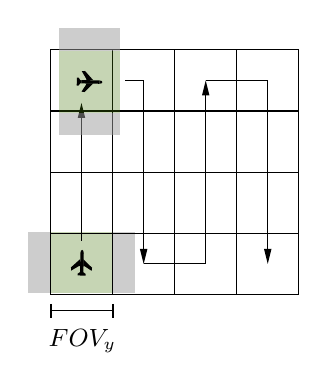
\begin{tikzpicture}[x=0.75pt,y=0.75pt,yscale=-1,xscale=1]
			%uncomment if require: \path (0,300); %set diagram left start at 0, and has height of 300
			
			%Shape: Rectangle [id:dp036802263347778474] 
			\draw  [draw opacity=0][fill={rgb, 255:red, 65; green, 117; blue, 5 }  ,fill opacity=0.3 ] (91.4,162.11) -- (121.3,162.11) -- (121.3,191.57) -- (91.4,191.57) -- cycle ;
			%Shape: Chord [id:dp8311663081836851] 
			\draw  [draw opacity=0][fill={rgb, 255:red, 0; green, 0; blue, 0 }  ,fill opacity=1 ] (105.79,172.1) .. controls (105.79,172.1) and (105.79,172.1) .. (105.79,172.1) .. controls (105.8,171.29) and (106.18,170.63) .. (106.62,170.64) .. controls (107.06,170.66) and (107.41,171.32) .. (107.39,172.14) -- cycle ;
			%Shape: Rectangle [id:dp8012179965756234] 
			\draw  [draw opacity=0][fill={rgb, 255:red, 0; green, 0; blue, 0 }  ,fill opacity=1 ] (107.39,172.14) -- (107.23,180.82) -- (105.62,180.78) -- (105.78,172.1) -- cycle ;
			%Shape: Chord [id:dp46276085808629674] 
			\draw  [draw opacity=0][fill={rgb, 255:red, 0; green, 0; blue, 0 }  ,fill opacity=1 ] (107.23,180.82) .. controls (107.23,180.82) and (107.23,180.82) .. (107.23,180.82) .. controls (107.21,181.63) and (106.84,182.28) .. (106.4,182.27) .. controls (105.95,182.26) and (105.61,181.59) .. (105.62,180.78) -- cycle ;
			%Shape: Boxed Polygon [id:dp33577441359912386] 
			\draw  [draw opacity=0][fill={rgb, 255:red, 0; green, 0; blue, 0 }  ,fill opacity=1 ] (111.19,180.75) -- (107.86,178.55) -- (107.16,178.35) -- (107.21,175.15) -- (111.37,179.23) -- cycle ;
			%Shape: Boxed Polygon [id:dp4613372486056908] 
			\draw  [draw opacity=0][fill={rgb, 255:red, 0; green, 0; blue, 0 }  ,fill opacity=1 ] (101.36,180.59) -- (104.88,178.52) -- (105.61,178.35) -- (105.65,175.11) -- (101.22,179.05) -- cycle ;
			%Shape: Boxed Polygon [id:dp09882619727387199] 
			\draw  [draw opacity=0][fill={rgb, 255:red, 0; green, 0; blue, 0 }  ,fill opacity=1 ] (108.27,182.2) -- (108.23,183.06) -- (104.44,182.93) -- (104.47,182.1) -- (106.42,180.8) -- cycle ;
			
			%Shape: Rectangle [id:dp43518650932458014] 
			\draw  [draw opacity=0][fill={rgb, 255:red, 155; green, 155; blue, 155 }  ,fill opacity=0.5 ] (121.3,162.07) -- (132.06,162.07) -- (132.06,191.61) -- (121.3,191.61) -- cycle ;
			%Shape: Rectangle [id:dp898186670672066] 
			\draw  [draw opacity=0][fill={rgb, 255:red, 155; green, 155; blue, 155 }  ,fill opacity=0.5 ] (80.64,162.07) -- (91.4,162.07) -- (91.4,191.61) -- (80.64,191.61) -- cycle ;
			
			%Shape: Rectangle [id:dp12911688161174095] 
			\draw   (91.4,74.26) -- (121.3,74.26) -- (121.3,103.72) -- (91.4,103.72) -- cycle ;
			%Shape: Rectangle [id:dp778307202398685] 
			\draw   (121.3,74.26) -- (151.2,74.26) -- (151.2,103.72) -- (121.3,103.72) -- cycle ;
			%Shape: Rectangle [id:dp5920975737411569] 
			\draw   (151.2,74.26) -- (181.1,74.26) -- (181.1,103.72) -- (151.2,103.72) -- cycle ;
			%Shape: Rectangle [id:dp7108929033014086] 
			\draw   (91.4,103.72) -- (121.3,103.72) -- (121.3,133.18) -- (91.4,133.18) -- cycle ;
			%Shape: Rectangle [id:dp8152064023887235] 
			\draw   (91.4,133.18) -- (121.3,133.18) -- (121.3,162.64) -- (91.4,162.64) -- cycle ;
			%Shape: Rectangle [id:dp01596026185419297] 
			\draw   (181.1,162.64) -- (211,162.64) -- (211,192.11) -- (181.1,192.11) -- cycle ;
			%Shape: Rectangle [id:dp7327882569457931] 
			\draw   (121.3,103.72) -- (151.2,103.72) -- (151.2,133.18) -- (121.3,133.18) -- cycle ;
			%Shape: Rectangle [id:dp11348064360337196] 
			\draw   (121.3,133.18) -- (151.2,133.18) -- (151.2,162.64) -- (121.3,162.64) -- cycle ;
			%Shape: Rectangle [id:dp5274571336670886] 
			\draw   (151.2,133.18) -- (181.1,133.18) -- (181.1,162.64) -- (151.2,162.64) -- cycle ;
			%Shape: Rectangle [id:dp1361244585482333] 
			\draw   (151.2,103.72) -- (181.1,103.72) -- (181.1,133.18) -- (151.2,133.18) -- cycle ;
			%Shape: Rectangle [id:dp8698952772815938] 
			\draw   (91.4,162.64) -- (121.3,162.64) -- (121.3,192.11) -- (91.4,192.11) -- cycle ;
			%Shape: Rectangle [id:dp8275138362077274] 
			\draw   (121.3,162.64) -- (151.2,162.64) -- (151.2,192.11) -- (121.3,192.11) -- cycle ;
			%Shape: Rectangle [id:dp5045016465037775] 
			\draw   (151.2,162.64) -- (181.1,162.64) -- (181.1,192.11) -- (151.2,192.11) -- cycle ;
			%Shape: Rectangle [id:dp5051198991702088] 
			\draw   (181.1,133.18) -- (211,133.18) -- (211,162.64) -- (181.1,162.64) -- cycle ;
			%Shape: Rectangle [id:dp9607013415516779] 
			\draw   (181.1,103.72) -- (211,103.72) -- (211,133.18) -- (181.1,133.18) -- cycle ;
			%Shape: Rectangle [id:dp5794670437040133] 
			\draw   (181.1,74.26) -- (211,74.26) -- (211,103.72) -- (181.1,103.72) -- cycle ;
			%Straight Lines [id:da9321367214575229] 
			\draw    (106.29,166.14) -- (106.29,101.86) ;
			\draw [shift={(106.29,99.86)}, rotate = 450] [fill={rgb, 255:red, 0; green, 0; blue, 0 }  ][line width=0.08]  [draw opacity=0] (7.2,-1.8) -- (0,0) -- (7.2,1.8) -- cycle    ;
			%Straight Lines [id:da40799678234401227] 
			\draw    (166.15,177.38) -- (166.15,90.99) ;
			\draw [shift={(166.15,88.99)}, rotate = 450] [fill={rgb, 255:red, 0; green, 0; blue, 0 }  ][line width=0.08]  [draw opacity=0] (7.2,-1.8) -- (0,0) -- (7.2,1.8) -- cycle    ;
			%Straight Lines [id:da2047551510485104] 
			\draw    (136.25,89.23) -- (127.29,89.23) ;
			%Shape: Rectangle [id:dp8051835391549806] 
			\draw  [draw opacity=0][fill={rgb, 255:red, 65; green, 117; blue, 5 }  ,fill opacity=0.3 ] (124.94,74.61) -- (124.94,104.51) -- (95.48,104.51) -- (95.48,74.61) -- cycle ;
			%Shape: Chord [id:dp01440978675599247] 
			\draw  [draw opacity=0][fill={rgb, 255:red, 0; green, 0; blue, 0 }  ,fill opacity=1 ] (114.95,88.99) .. controls (114.95,88.99) and (114.95,88.99) .. (114.95,88.99) .. controls (115.76,89.01) and (116.42,89.38) .. (116.4,89.83) .. controls (116.39,90.27) and (115.72,90.61) .. (114.91,90.6) -- cycle ;
			%Shape: Rectangle [id:dp47820815125081073] 
			\draw  [draw opacity=0][fill={rgb, 255:red, 0; green, 0; blue, 0 }  ,fill opacity=1 ] (114.91,90.6) -- (106.23,90.43) -- (106.27,88.82) -- (114.95,88.99) -- cycle ;
			%Shape: Chord [id:dp5606590464537962] 
			\draw  [draw opacity=0][fill={rgb, 255:red, 0; green, 0; blue, 0 }  ,fill opacity=1 ] (106.23,90.43) .. controls (105.42,90.42) and (104.77,90.05) .. (104.78,89.6) .. controls (104.79,89.16) and (105.46,88.81) .. (106.27,88.83) -- cycle ;
			%Shape: Boxed Polygon [id:dp9266491051896144] 
			\draw  [draw opacity=0][fill={rgb, 255:red, 0; green, 0; blue, 0 }  ,fill opacity=1 ] (106.3,94.4) -- (108.5,91.06) -- (108.7,90.37) -- (111.9,90.42) -- (107.82,94.58) -- cycle ;
			%Shape: Boxed Polygon [id:dp034397174811206854] 
			\draw  [draw opacity=0][fill={rgb, 255:red, 0; green, 0; blue, 0 }  ,fill opacity=1 ] (106.46,84.57) -- (108.53,88.09) -- (108.7,88.81) -- (111.94,88.86) -- (108,84.43) -- cycle ;
			%Shape: Boxed Polygon [id:dp03511489675126511] 
			\draw  [draw opacity=0][fill={rgb, 255:red, 0; green, 0; blue, 0 }  ,fill opacity=1 ] (104.85,91.48) -- (103.99,91.43) -- (104.12,87.65) -- (104.95,87.68) -- (106.25,89.63) -- cycle ;
			
			%Shape: Rectangle [id:dp6507888601892564] 
			\draw  [draw opacity=0][fill={rgb, 255:red, 155; green, 155; blue, 155 }  ,fill opacity=0.5 ] (124.98,104.51) -- (124.98,115.27) -- (95.44,115.27) -- (95.44,104.51) -- cycle ;
			%Shape: Rectangle [id:dp5268420170616126] 
			\draw  [draw opacity=0][fill={rgb, 255:red, 155; green, 155; blue, 155 }  ,fill opacity=0.5 ] (124.98,63.84) -- (124.98,74.61) -- (95.44,74.61) -- (95.44,63.84) -- cycle ;
			
			%Straight Lines [id:da6678654382408558] 
			\draw    (166.15,177.38) -- (136.25,177.38) ;
			%Straight Lines [id:da2744825079592068] 
			\draw    (166.15,88.99) -- (196.05,88.99) ;
			%Straight Lines [id:da1430427767977791] 
			\draw    (196.05,88.99) -- (196.05,175.38) ;
			\draw [shift={(196.05,177.38)}, rotate = 270] [fill={rgb, 255:red, 0; green, 0; blue, 0 }  ][line width=0.08]  [draw opacity=0] (7.2,-1.8) -- (0,0) -- (7.2,1.8) -- cycle    ;
			%Straight Lines [id:da45865584522885094] 
			\draw    (136.25,88.99) -- (136.25,175.38) ;
			\draw [shift={(136.25,177.38)}, rotate = 270] [fill={rgb, 255:red, 0; green, 0; blue, 0 }  ][line width=0.08]  [draw opacity=0] (7.2,-1.8) -- (0,0) -- (7.2,1.8) -- cycle    ;
			%Straight Lines [id:da8017813803709761] 
			\draw    (91.4,200) -- (121.4,200) ;
			\draw [shift={(121.4,200)}, rotate = 180] [color={rgb, 255:red, 0; green, 0; blue, 0 }  ][line width=0.75]    (0,3.35) -- (0,-3.35)   ;
			\draw [shift={(91.4,200)}, rotate = 180] [color={rgb, 255:red, 0; green, 0; blue, 0 }  ][line width=0.75]    (0,3.35) -- (0,-3.35)   ;
			
			% Text Node
			\draw (89.2,207.6) node [anchor=north west][inner sep=0.75pt]  [font=\small]  {$FOV_{y}$};
			
		\end{tikzpicture}
		\caption{Square discretisation}
		\label{fig:Overlap-sqr}
	\end{subfigure}
	\hfill
	\begin{subfigure}[b]{0.6\textwidth}
		\centering
		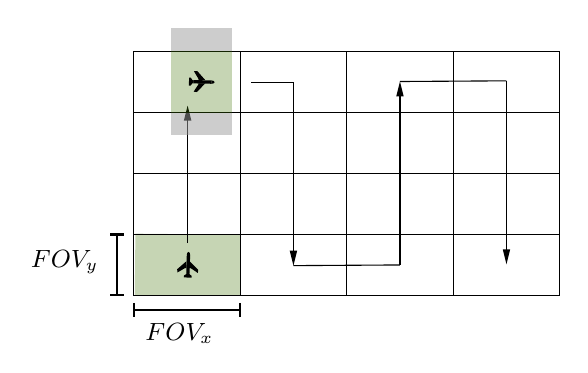
\begin{tikzpicture}[x=0.75pt,y=0.75pt,yscale=-1,xscale=1]
			%uncomment if require: \path (0,300); %set diagram left start at 0, and has height of 300
			
			%Shape: Rectangle [id:dp1592240079509375] 
			\draw  [draw opacity=0][fill={rgb, 255:red, 65; green, 117; blue, 5 }  ,fill opacity=0.3 ] (256.84,181.82) -- (307.71,182.34) -- (307.41,211.8) -- (256.54,211.29) -- cycle ;
			%Shape: Chord [id:dp027006860973721514] 
			\draw  [draw opacity=0][fill={rgb, 255:red, 0; green, 0; blue, 0 }  ,fill opacity=1 ] (281.6,192.06) .. controls (281.62,191.24) and (282,190.6) .. (282.44,190.61) .. controls (282.88,190.63) and (283.22,191.3) .. (283.2,192.11) -- cycle ;
			%Shape: Rectangle [id:dp5979870900127169] 
			\draw  [draw opacity=0][fill={rgb, 255:red, 0; green, 0; blue, 0 }  ,fill opacity=1 ] (283.2,192.11) -- (282.95,200.79) -- (281.34,200.73) -- (281.59,192.06) -- cycle ;
			%Shape: Chord [id:dp2765435991887346] 
			\draw  [draw opacity=0][fill={rgb, 255:red, 0; green, 0; blue, 0 }  ,fill opacity=1 ] (282.95,200.79) .. controls (282.92,201.6) and (282.54,202.25) .. (282.1,202.24) .. controls (281.66,202.22) and (281.32,201.55) .. (281.34,200.73) -- cycle ;
			%Shape: Boxed Polygon [id:dp6872706935659367] 
			\draw  [draw opacity=0][fill={rgb, 255:red, 0; green, 0; blue, 0 }  ,fill opacity=1 ] (286.91,200.76) -- (283.6,198.53) -- (282.91,198.32) -- (282.99,195.12) -- (287.11,199.24) -- cycle ;
			%Shape: Boxed Polygon [id:dp5311750689290109] 
			\draw  [draw opacity=0][fill={rgb, 255:red, 0; green, 0; blue, 0 }  ,fill opacity=1 ] (277.09,200.5) -- (280.62,198.47) -- (281.35,198.31) -- (281.43,195.07) -- (276.96,198.96) -- cycle ;
			%Shape: Boxed Polygon [id:dp9447821201006807] 
			\draw  [draw opacity=0][fill={rgb, 255:red, 0; green, 0; blue, 0 }  ,fill opacity=1 ] (283.98,202.18) -- (283.92,203.04) -- (280.14,202.88) -- (280.18,202.05) -- (282.14,200.76) -- cycle ;
			
			
			%Shape: Rectangle [id:dp49983792011863337] 
			\draw   (255.97,94.15) -- (307.3,94.15) -- (307.3,123.51) -- (255.97,123.51) -- cycle ;
			%Shape: Rectangle [id:dp8807821798790052] 
			\draw   (307.3,94.15) -- (358.63,94.15) -- (358.63,123.51) -- (307.3,123.51) -- cycle ;
			%Shape: Rectangle [id:dp8181512728288265] 
			\draw   (358.63,94.15) -- (409.96,94.15) -- (409.96,123.51) -- (358.63,123.51) -- cycle ;
			%Shape: Rectangle [id:dp09547819591891549] 
			\draw   (255.97,123.51) -- (307.3,123.51) -- (307.3,152.86) -- (255.97,152.86) -- cycle ;
			%Shape: Rectangle [id:dp1985429505890559] 
			\draw   (255.97,152.86) -- (307.3,152.86) -- (307.3,182.22) -- (255.97,182.22) -- cycle ;
			%Shape: Rectangle [id:dp5422527345143757] 
			\draw   (409.96,182.22) -- (461.29,182.22) -- (461.29,211.57) -- (409.96,211.57) -- cycle ;
			%Shape: Rectangle [id:dp332416764045272] 
			\draw   (307.3,123.51) -- (358.63,123.51) -- (358.63,152.86) -- (307.3,152.86) -- cycle ;
			%Shape: Rectangle [id:dp36287337689551014] 
			\draw   (307.3,152.86) -- (358.63,152.86) -- (358.63,182.22) -- (307.3,182.22) -- cycle ;
			%Shape: Rectangle [id:dp4697135024528536] 
			\draw   (358.63,152.86) -- (409.96,152.86) -- (409.96,182.22) -- (358.63,182.22) -- cycle ;
			%Shape: Rectangle [id:dp1298855569227555] 
			\draw   (358.63,123.51) -- (409.96,123.51) -- (409.96,152.86) -- (358.63,152.86) -- cycle ;
			%Shape: Rectangle [id:dp8663339040779854] 
			\draw   (255.97,182.22) -- (307.3,182.22) -- (307.3,211.57) -- (255.97,211.57) -- cycle ;
			%Shape: Rectangle [id:dp9437211813054305] 
			\draw   (307.3,182.22) -- (358.63,182.22) -- (358.63,211.57) -- (307.3,211.57) -- cycle ;
			%Shape: Rectangle [id:dp810113535837834] 
			\draw   (358.63,182.22) -- (409.96,182.22) -- (409.96,211.57) -- (358.63,211.57) -- cycle ;
			%Shape: Rectangle [id:dp5562129843015806] 
			\draw   (409.96,152.86) -- (461.29,152.86) -- (461.29,182.22) -- (409.96,182.22) -- cycle ;
			%Shape: Rectangle [id:dp8187981325254521] 
			\draw   (409.96,123.51) -- (461.29,123.51) -- (461.29,152.86) -- (409.96,152.86) -- cycle ;
			%Shape: Rectangle [id:dp6245482862531306] 
			\draw   (409.96,94.15) -- (461.29,94.15) -- (461.29,123.51) -- (409.96,123.51) -- cycle ;
			
			%Straight Lines [id:da41795839579175675] 
			\draw    (282,186.43) -- (282,122.14) ;
			\draw [shift={(282,120.14)}, rotate = 450] [fill={rgb, 255:red, 0; green, 0; blue, 0 }  ][line width=0.08]  [draw opacity=0] (7.2,-1.8) -- (0,0) -- (7.2,1.8) -- cycle    ;
			%Straight Lines [id:da1509716304633384] 
			\draw    (332.96,108.83) -- (312.68,108.83) ;
			%Straight Lines [id:da48049309446832655] 
			\draw    (332.96,108.83) -- (332.96,195.22) ;
			\draw [shift={(332.96,197.22)}, rotate = 270] [fill={rgb, 255:red, 0; green, 0; blue, 0 }  ][line width=0.08]  [draw opacity=0] (7.2,-1.8) -- (0,0) -- (7.2,1.8) -- cycle    ;
			%Straight Lines [id:da4231981271606413] 
			\draw    (384.29,196.89) -- (332.96,197.22) ;
			%Straight Lines [id:da4546308979435414] 
			\draw    (384.29,196.89) -- (384.29,110.51) ;
			\draw [shift={(384.29,108.51)}, rotate = 450] [fill={rgb, 255:red, 0; green, 0; blue, 0 }  ][line width=0.08]  [draw opacity=0] (7.2,-1.8) -- (0,0) -- (7.2,1.8) -- cycle    ;
			%Straight Lines [id:da10063088031705991] 
			\draw    (435.62,108.18) -- (384.29,108.51) ;
			%Straight Lines [id:da8147890256777217] 
			\draw    (435.62,108.18) -- (435.62,194.57) ;
			\draw [shift={(435.62,196.57)}, rotate = 270] [fill={rgb, 255:red, 0; green, 0; blue, 0 }  ][line width=0.08]  [draw opacity=0] (7.2,-1.8) -- (0,0) -- (7.2,1.8) -- cycle    ;
			%Shape: Rectangle [id:dp7310476894921445] 
			\draw  [draw opacity=0][fill={rgb, 255:red, 65; green, 117; blue, 5 }  ,fill opacity=0.3 ] (303.54,93.61) -- (303.54,123.51) -- (274.08,123.51) -- (274.08,93.61) -- cycle ;
			%Shape: Chord [id:dp19645121488474926] 
			\draw  [draw opacity=0][fill={rgb, 255:red, 0; green, 0; blue, 0 }  ,fill opacity=1 ] (293.55,107.99) .. controls (294.36,108.01) and (295.02,108.38) .. (295,108.83) .. controls (294.99,109.27) and (294.32,109.61) .. (293.51,109.6) -- cycle ;
			%Shape: Rectangle [id:dp05174583825785106] 
			\draw  [draw opacity=0][fill={rgb, 255:red, 0; green, 0; blue, 0 }  ,fill opacity=1 ] (293.51,109.6) -- (284.83,109.43) -- (284.87,107.82) -- (293.55,107.99) -- cycle ;
			%Shape: Chord [id:dp1661582095490599] 
			\draw  [draw opacity=0][fill={rgb, 255:red, 0; green, 0; blue, 0 }  ,fill opacity=1 ] (284.83,109.43) .. controls (284.02,109.42) and (283.37,109.05) .. (283.38,108.6) .. controls (283.39,108.16) and (284.06,107.81) .. (284.87,107.83) -- cycle ;
			%Shape: Boxed Polygon [id:dp018588797866418538] 
			\draw  [draw opacity=0][fill={rgb, 255:red, 0; green, 0; blue, 0 }  ,fill opacity=1 ] (284.9,113.4) -- (287.1,110.06) -- (287.3,109.37) -- (290.5,109.42) -- (286.42,113.58) -- cycle ;
			%Shape: Boxed Polygon [id:dp3166422244467362] 
			\draw  [draw opacity=0][fill={rgb, 255:red, 0; green, 0; blue, 0 }  ,fill opacity=1 ] (285.06,103.57) -- (287.13,107.09) -- (287.3,107.81) -- (290.54,107.86) -- (286.6,103.43) -- cycle ;
			%Shape: Boxed Polygon [id:dp7707267480495361] 
			\draw  [draw opacity=0][fill={rgb, 255:red, 0; green, 0; blue, 0 }  ,fill opacity=1 ] (283.45,110.48) -- (282.59,110.43) -- (282.72,106.65) -- (283.55,106.68) -- (284.85,108.63) -- cycle ;
			
			%Shape: Rectangle [id:dp26082048868605323] 
			\draw  [draw opacity=0][fill={rgb, 255:red, 155; green, 155; blue, 155 }  ,fill opacity=0.5 ] (303.58,123.51) -- (303.58,134.27) -- (274.04,134.27) -- (274.04,123.51) -- cycle ;
			%Shape: Rectangle [id:dp570071469284922] 
			\draw  [draw opacity=0][fill={rgb, 255:red, 155; green, 155; blue, 155 }  ,fill opacity=0.5 ] (303.58,82.84) -- (303.58,93.61) -- (274.04,93.61) -- (274.04,82.84) -- cycle ;
			
			%Straight Lines [id:da1628094381777676] 
			\draw    (247.97,182.22) -- (247.97,211.57) ;
			\draw [shift={(247.97,211.57)}, rotate = 270] [color={rgb, 255:red, 0; green, 0; blue, 0 }  ][line width=0.75]    (0,3.35) -- (0,-3.35)   ;
			\draw [shift={(247.97,182.22)}, rotate = 270] [color={rgb, 255:red, 0; green, 0; blue, 0 }  ][line width=0.75]    (0,3.35) -- (0,-3.35)   ;
			%Straight Lines [id:da97063001945603] 
			\draw    (255.97,218.57) -- (307.3,218.57) ;
			\draw [shift={(307.3,218.57)}, rotate = 180] [color={rgb, 255:red, 0; green, 0; blue, 0 }  ][line width=0.75]    (0,3.35) -- (0,-3.35)   ;
			\draw [shift={(255.97,218.57)}, rotate = 180] [color={rgb, 255:red, 0; green, 0; blue, 0 }  ][line width=0.75]    (0,3.35) -- (0,-3.35)   ;
			
			% Text Node
			\draw (260.4,223.8) node [anchor=north west][inner sep=0.75pt]  [font=\small]  {$FOV_{x}$};
			% Text Node
			\draw (205.2,188.6) node [anchor=north west][inner sep=0.75pt]  [font=\small]  {$FOV_{y}$};
			
			
		\end{tikzpicture}
		\caption{Rectangular discretisation}
		\label{fig:Overlap-rect}
	\end{subfigure}
	\caption{Diagrams showing cross track overlap for camera Field of View for different discretisation techniques.}
\end{figure}

% TODO: Section where it is applied to different camera scenarios
\section{Implementation with Different Cameras}
\label{sec:ER-App}
% mention how dynamic constraints change everything - with this discretisation the asumption is that UAV can make 90 degree turns. This may be possible for some UAVs, but not while maintaining a constant velocity. Maintaining constant is more desireable because it consumes less energy. Mention how it is covered in a later section.



\chapter{Divide Areas Algorithm}
\label{chp:DARP}
In this project, the distributed method of multi-robot coverage path planning is implemented. Several different algorithms of this type are discussed in Section \ref{sec:LR Ditributed MCPP}. The algorithm being discussed in this chapter is briefly addressed in Section \ref{sec:LR DARP}. Section \ref{sec:DARP bg} addresses the algorithm in more detail, and Section \ref{sec:DARP dist} discusses the implementation of the algorithm with different distance measures. Section \ref{sec:DARP implement} then goes on to discuss the implementation of this algorithm in the context of this project.
\section{Background Theory}
% TODO: Figure out the subheadings here
\label{sec:DARP bg}
Grid-based coverage path planning can be implemented using a number of different methods. The Voronoi partition method of Section \ref{sec:LR-Voronoi} and the \acl{mstc} method of Section \ref{sec:LR-MSTC} are good examples. Both of these also fall into the distributed category. The \acl{ai} techniques of Section \ref{sec:LR-mAI} and the \acl{mfc} method described in Section \ref{sec:LR MFC} are counter examples of the non-distributed variety.

Naturally, achieving the most optimal solution possible would be most desirable. The authors of the divide areas algorithm described in this section, propose a set of requirements for optimal coverage path planning using a grid-based approach \cite{DARP2017}. These fundamental conditions, as they call them, are listed below.
\begin{enumerate}
\item Every cell in the environment, that is not classified as an object, must be covered. This is known as complete coverage.
\item Each cell in the environment must only be visited once, and only by one of the robots. This is known as the non-backtracking requirement.
\item Each robot should have as close to an equal amount of cells as possible assigned to it for covering. Their sets of cells should be of roughly the same size.
\item The sets of cells assigned to each robot should be a connected sub-region. This means that when generating a path to cover the cells within its set, a robot would not need to traverse the sub-region of another robot to reach its own.
\item The initial position of each robot should be contained within the set of cells assigned to it. This means that a robot would not need to traverse another robot's sub-region to reach its sub-region for coverage.
\end{enumerate}
The authors developed a methodology to achieve these optimal conditions. They called it the \ac{darp}. Their solution seeks to divide a known environment containing static obstacles into contiguous sub-regions. These regions are formed based on the robot starting positions so that each robot starts within one of the regions.

The solution is found in an iterative manner and it converges to where the sub-regions are cohesive and roughly the same size. \ac{darp} only divides the environment appropriately between robots. A single robot \ac{cpp} algorithm can then be utilized to achieve complete coverage of each sub-region, which translates to complete coverage of the whole environment.
% TODO: Maybe mention something about the EXISTENCE of solutions
\subsection{Algorithm Description}
The algorithm works on a two-dimensional environment that is divided into discrete cells. Once the discretisation is complete, the algorithm starts by operating similar to a Voronoi partition. It constructs a matrix for each robot with the same dimension as the environment. The authors refer to these as the Evaluation Matrices ($E_i$). They contain the distances from each cell in the environment to the respective robots. Euclidean distance was used as the distance measure.                                                                                                                                                                                                                                                                                                                                                                                                                                                                                                                                                                             
\begin{figure}[h!]
\centering
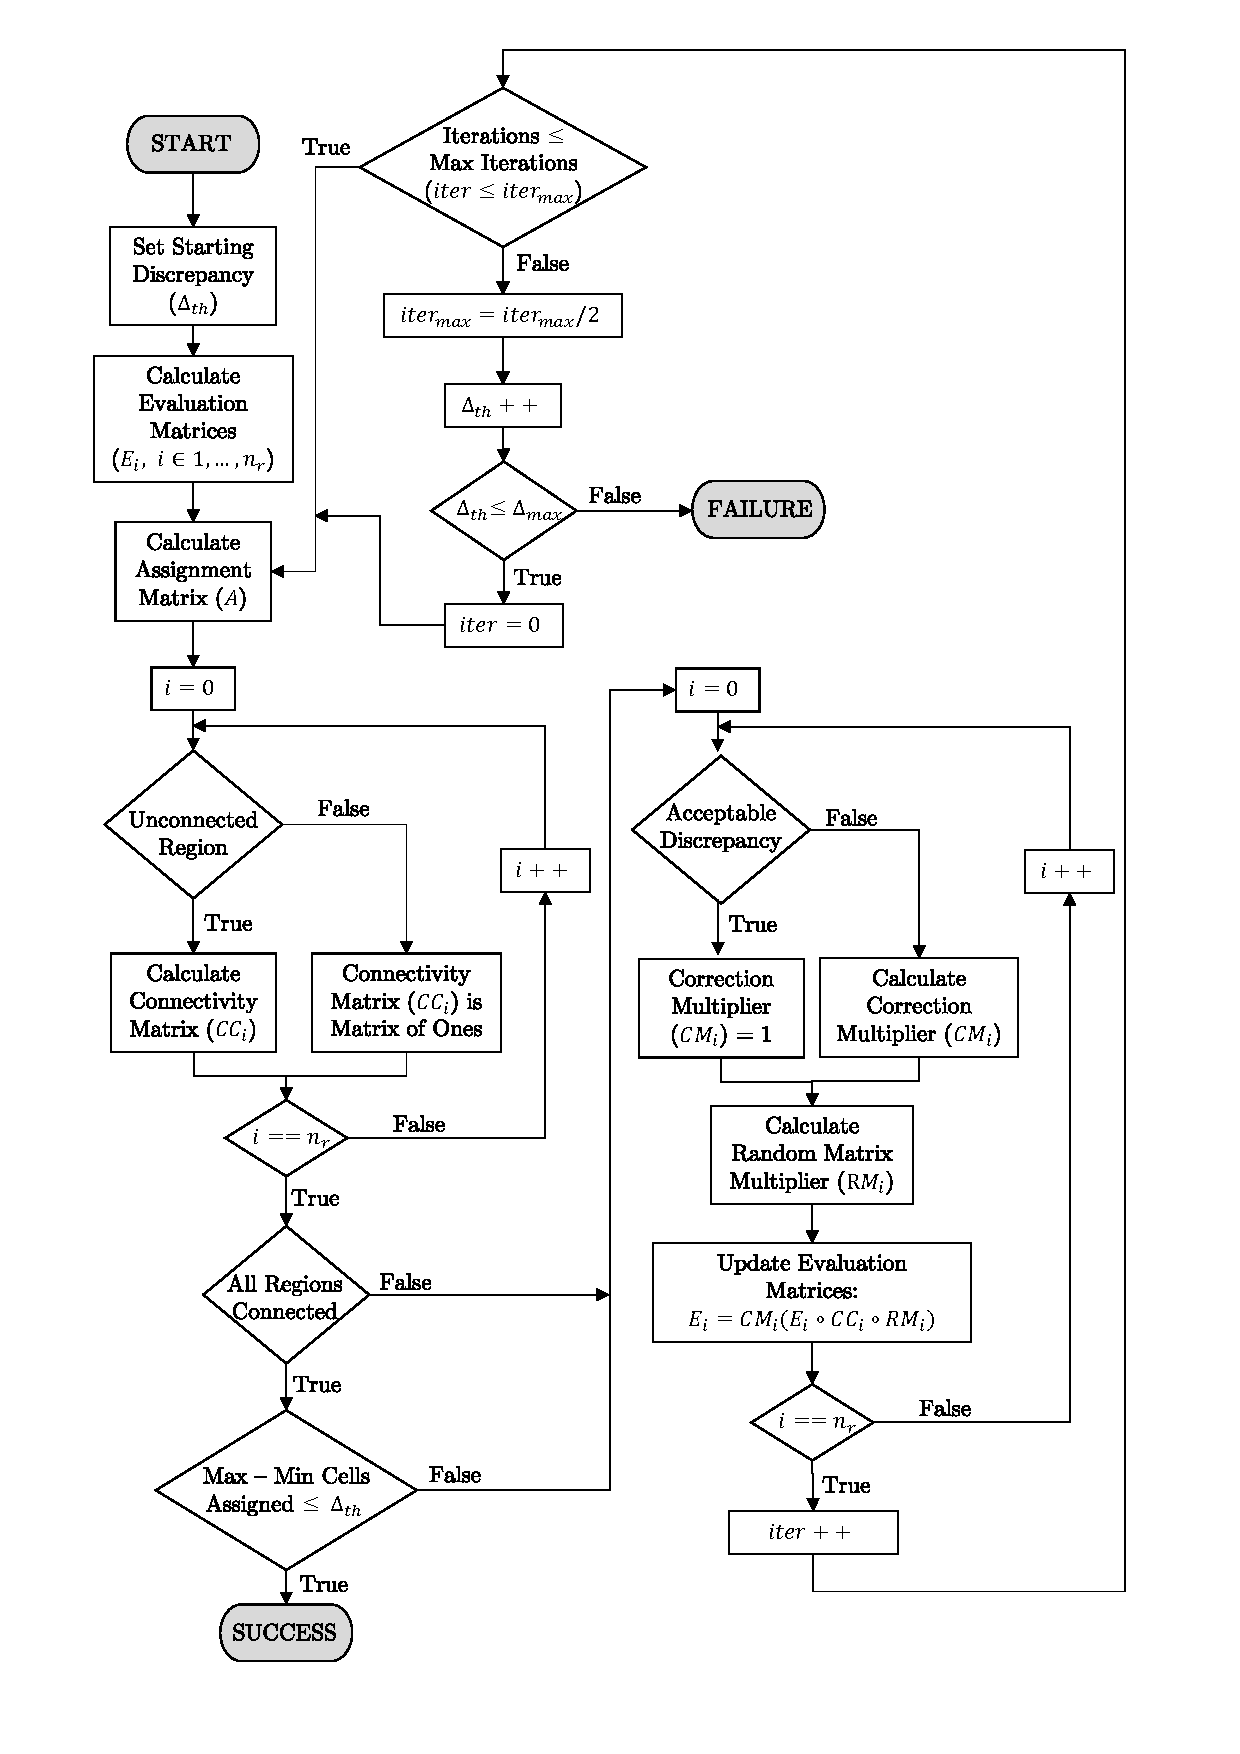
\includegraphics[scale=0.8,trim={1.5cm 0 1.5cm 0},clip]{figs/DARP_Diagram3.pdf}
\caption{Flow diagram representing the logic for DARP.}
\label{fig:DARP}
\end{figure}
\section{Implementation}
\label{sec:DARP implement}
For this implementation, two alterations were made to the \ac{darp} algorithm. The first was a minor change involving an enclosed region checker. The capability was added to detect an enclosed space within the environment and treat it as an obstacle. This change will not be discussed in detail. The second change was adding the ability to use different distance measures, aside from the Euclidean distance measure it was originally implemented with. 

This section has three subsections, starting with a section discussing the suitability of \ac{darp} for this application. The next section goes into detail regarding the different distance measure implementations, and the final section shows some illustrative results where \ac{darp} is implemented in different scenarios.
% TODO: Maybe add section looking at cc and rl values (remember to address section breakdowns then)
% TODO: Mention a bit more about enclosed space handler if you want
\subsection{Algorithm Suitability and Limitations}
% TODO: Add more references - refer back to papers in literature review maybe e.g. online ones for SAR
DARP is a grid-based, distributed , offline algorithm. In this project it has been chosen as an appropriate algorithm in the context of \ac{sar} for a number of different reasons. 
% Why is DARP Appropriate for this problem - grid, offline, distributed

% Grid based
Many existing algorithms make use of a grid-based representation of the environment. In offline approaches, this is convenient to represent the environment. One downside is that if the grid resolution is too low, the representation of the environment becomes less accurate. This is why it is called an approximate approach \cite{Choset2001}. 

The low resolution can be combated by introducing some sensor overlap, or by simply ensuring the resolution is very high. However, higher resolution means more computational power is required, so this should not be done irresponsibly.

% Distributed - justification
Because it is a distributed method, each robot travels only within its allocated sub-region. These regions don't overlap, meaning that the robots will never collide, provided they follow their planned path. Therefore, it removes a layer of complexity that often gets added with multi-robot approaches. So long as the \acp{uav} follow their paths within a reasonable margin of error, they will never collide with one-another.

% Offline - justification (Centralized and decentralized)
It is also an offline approach to \ac{cpp}, so the environment is known prior to the planning phase. The divide areas algorithm and the sub-region coverage algorithm, which is discussed in Chapter \ref{chp:Subregion-Coverage}, are both included in the planning phase. 

Online approaches are generally considered appropriate for dynamic environments. This could refer to any amount of objects in motion within the environment that need to be avoided. Often times, the other \acp{uav} in the environment are modeled as dynamic obstacles from the perspective of a single \ac{uav}. With a distributed approach, this would be unnecessary, because the \ac{uav} paths will never cross one-another. 

Sometimes, online approaches are deemed appropriate because inputting the environment into the planner a priori is considered too costly. In the case of \ac{sar}, it is reasonable to assume that plotting the environment from a bird's eye view is uncomplicated due to available satellite imagery. 

There is generally enough information to map out the aerial environment beforehand, seen as \acp{uav} fly high enough to avoid most obstructions in an environment. Obstacles, in this type of scenario, could be a physical obstruction like power lines or a mountain in a plain. They could also be no-fly zones such as restricted air space or populous regions.

It should be noted that in online approaches, information sharing becomes quite critical. If the \acp{uav} have a large enough communication range they can follow a centralized approach, where all data is sent to a central command station or \ac{uav}, that plans all their paths simultaneously. They could also all operate independently and simply share information when in range, which is a decentralized approach. \cite{Zhang2020}

For the offline case, approaches can generally be viewed as centralized. Their paths are planned in full beforehand, and the only thing that requires monitoring during flight, is whether they follow this trajectory within an acceptable margin of error to avoid collisions, and achieve good coverage. For \ac{sar} it would also be beneficial to receive real-time data that can be used to locate a target.

This project develops the algorithm for \ac{cpp} in the context of \ac{sar}. The trajectory following control system and target detection method will become relevant if this project is extended to a physical implementation in future. Other dynamic elements in the environment, such as birds or other air vehicles, can also be accounted for using some form of collision avoidance. This could mean that the algorithm becomes more of a hybrid approach, depending on how much of the functionality is implemented online.

\subsection{Distance Measure Comparisons}
\label{sec:DARP dist}
% Include thing where you compare distance measures and how it effects number of iterations

\subsection{Implementation with Different Environments}
% Different Environments, Obstacle Dispersion and Robot Dispersion
\chapter{Subregion Coverage Technique}
\label{chp:Subregion-Coverage}


%%%%%%%%%%%%%%%%%%%%%%%%%%%%%%%%%%%%%%%%%%%%%%%%%%%%%%%%%%%%%%%%%%%%%%%
\section{Background}

% Refer back to the literature review

\section{Spanning Tree Generation}

% Mention the small cells and the large cells

\section{Spanning Tree Circumnavigation}
Once the tree has been generated, the circumnavigation is achieved in two phases. Initially, a series of arrows are generated to represent a clockwise motion around the tree. This looks similar to a directed graph, because the edges are essentially assigned direction. However, because these arrows are used to generate a path for tree circumnavigation, there will be two arrows on each edge and the order in which they are used is crucial. In the second phase, these arrows are used to generate the way-points necessary to circumnavigate the tree.

A convention was formed in order to generate the arrows and way-points consistently. Firstly, once the tree is generated, a starting node is chosen. From this node, a walk is done from one node to the next to form arrows. These arrows are generated in such a way that they can be used to represent a clockwise motion around the tree. Keeping this clockwise convention in mind, way-points are generated for each arrow. 

The direction an arrow points always represents a forward motion. If the next arrow is pointing in the same direction, it is considered a forward motion. Three other motions are possible, namely left, right and backward motions. It is important to note that, although backtracking is allowed for arrows, this is not the case for the way-points. A representation of how a reference frame would move with the arrows in the event of a right turn is shown in Figure \ref{fig:ref-frame}.

\begin{figure}[h!]
	\centering
	\tikzset{every picture/.style={line width=0.75pt}} %set default line width to 0.75pt        	
	\begin{tikzpicture}[x=0.75pt,y=0.75pt,yscale=-1,xscale=1]
		%uncomment if require: \path (0,428); %set diagram left start at 0, and has height of 428
		
		%Straight Lines [id:da22962018155747188] 
		\draw [color={rgb, 255:red, 208; green, 2; blue, 27 }  ,draw opacity=1 ]   (339.88,99.5) -- (284,99.5) ;
		%Straight Lines [id:da20659579397175154] 
		\draw [color={rgb, 255:red, 208; green, 2; blue, 27 }  ,draw opacity=1 ]   (150,166) -- (150,223.94) ;
		%Straight Lines [id:da29821586315410764] 
		\draw    (90,226) -- (210,226) ;
		%Straight Lines [id:da8192544007793721] 
		\draw    (150,286) -- (150,226) ;
		%Shape: Circle [id:dp35225972894210633] 
		\draw  [draw opacity=0][fill={rgb, 255:red, 0; green, 0; blue, 0 }  ,fill opacity=1 ] (144.95,226) .. controls (144.95,223.21) and (147.21,220.95) .. (150,220.95) .. controls (152.79,220.95) and (155.05,223.21) .. (155.05,226) .. controls (155.05,228.79) and (152.79,231.05) .. (150,231.05) .. controls (147.21,231.05) and (144.95,228.79) .. (144.95,226) -- cycle ;
		%Shape: Circle [id:dp9484671919378986] 
		\draw  [fill={rgb, 255:red, 0; green, 0; blue, 0 }  ,fill opacity=1 ] (210,226) .. controls (210,224.86) and (210.92,223.94) .. (212.06,223.94) .. controls (213.2,223.94) and (214.13,224.86) .. (214.13,226) .. controls (214.13,227.14) and (213.2,228.06) .. (212.06,228.06) .. controls (210.92,228.06) and (210,227.14) .. (210,226) -- cycle ;
		%Shape: Circle [id:dp833048521369973] 
		\draw  [fill={rgb, 255:red, 0; green, 0; blue, 0 }  ,fill opacity=1 ] (147.94,286) .. controls (147.94,284.86) and (148.86,283.94) .. (150,283.94) .. controls (151.14,283.94) and (152.06,284.86) .. (152.06,286) .. controls (152.06,287.14) and (151.14,288.06) .. (150,288.06) .. controls (148.86,288.06) and (147.94,287.14) .. (147.94,286) -- cycle ;
		%Shape: Circle [id:dp5683936728423231] 
		\draw  [color={rgb, 255:red, 208; green, 2; blue, 27 }  ,draw opacity=1 ][fill={rgb, 255:red, 208; green, 2; blue, 27 }  ,fill opacity=1 ] (147.94,168.06) .. controls (147.94,166.92) and (148.86,166) .. (150,166) .. controls (151.14,166) and (152.06,166.92) .. (152.06,168.06) .. controls (152.06,169.2) and (151.14,170.13) .. (150,170.13) .. controls (148.86,170.13) and (147.94,169.2) .. (147.94,168.06) -- cycle ;
		%Shape: Circle [id:dp6006706790162355] 
		\draw  [fill={rgb, 255:red, 0; green, 0; blue, 0 }  ,fill opacity=1 ] (90,226) .. controls (90,224.86) and (90.92,223.94) .. (92.06,223.94) .. controls (93.2,223.94) and (94.13,224.86) .. (94.13,226) .. controls (94.13,227.14) and (93.2,228.06) .. (92.06,228.06) .. controls (90.92,228.06) and (90,227.14) .. (90,226) -- cycle ;
		%Straight Lines [id:da6990176420132321] 
		\draw    (284,39.5) -- (284,159.5) ;
		%Straight Lines [id:da15438188613200365] 
		\draw    (224,99.5) -- (284,99.5) ;
		%Shape: Circle [id:dp6972525301538133] 
		\draw  [draw opacity=0][fill={rgb, 255:red, 0; green, 0; blue, 0 }  ,fill opacity=1 ] (284,94.45) .. controls (286.79,94.45) and (289.05,96.71) .. (289.05,99.5) .. controls (289.05,102.29) and (286.79,104.55) .. (284,104.55) .. controls (281.21,104.55) and (278.95,102.29) .. (278.95,99.5) .. controls (278.95,96.71) and (281.21,94.45) .. (284,94.45) -- cycle ;
		%Shape: Circle [id:dp400672837370456] 
		\draw  [fill={rgb, 255:red, 0; green, 0; blue, 0 }  ,fill opacity=1 ] (284,159.5) .. controls (285.14,159.5) and (286.06,160.42) .. (286.06,161.56) .. controls (286.06,162.7) and (285.14,163.63) .. (284,163.63) .. controls (282.86,163.63) and (281.94,162.7) .. (281.94,161.56) .. controls (281.94,160.42) and (282.86,159.5) .. (284,159.5) -- cycle ;
		%Shape: Circle [id:dp8987931435704095] 
		\draw  [fill={rgb, 255:red, 0; green, 0; blue, 0 }  ,fill opacity=1 ] (224,97.44) .. controls (225.14,97.44) and (226.06,98.36) .. (226.06,99.5) .. controls (226.06,100.64) and (225.14,101.56) .. (224,101.56) .. controls (222.86,101.56) and (221.94,100.64) .. (221.94,99.5) .. controls (221.94,98.36) and (222.86,97.44) .. (224,97.44) -- cycle ;
		%Shape: Circle [id:dp9066989908899119] 
		\draw  [color={rgb, 255:red, 208; green, 2; blue, 27 }  ,draw opacity=1 ][fill={rgb, 255:red, 208; green, 2; blue, 27 }  ,fill opacity=1 ] (341.94,97.44) .. controls (343.08,97.44) and (344,98.36) .. (344,99.5) .. controls (344,100.64) and (343.08,101.56) .. (341.94,101.56) .. controls (340.8,101.56) and (339.88,100.64) .. (339.88,99.5) .. controls (339.88,98.36) and (340.8,97.44) .. (341.94,97.44) -- cycle ;
		%Shape: Circle [id:dp8606951024205995] 
		\draw  [fill={rgb, 255:red, 0; green, 0; blue, 0 }  ,fill opacity=1 ] (284,39.5) .. controls (285.14,39.5) and (286.06,40.42) .. (286.06,41.56) .. controls (286.06,42.7) and (285.14,43.63) .. (284,43.63) .. controls (282.86,43.63) and (281.94,42.7) .. (281.94,41.56) .. controls (281.94,40.42) and (282.86,39.5) .. (284,39.5) -- cycle ;
		%Straight Lines [id:da29854683273675375] 
		\draw  [dash pattern={on 4.5pt off 4.5pt}]  (150,100) -- (200,100) ;
		%Straight Lines [id:da590718802691715] 
		\draw  [dash pattern={on 4.5pt off 4.5pt}]  (150,102) -- (150,140) ;
		\draw [shift={(150,100)}, rotate = 90] [fill={rgb, 255:red, 0; green, 0; blue, 0 }  ][line width=0.08]  [draw opacity=0] (12,-3) -- (0,0) -- (12,3) -- cycle    ;
		%Straight Lines [id:da6608297236594676] 
		\draw  [dash pattern={on 4.5pt off 4.5pt}]  (360,100) -- (448,100) ;
		\draw [shift={(450,100)}, rotate = 180] [fill={rgb, 255:red, 0; green, 0; blue, 0 }  ][line width=0.08]  [draw opacity=0] (12,-3) -- (0,0) -- (12,3) -- cycle    ;
		
		% Text Node
		\draw (217,218) node [anchor=north west][inner sep=0.75pt]   [align=left] {R};
		% Text Node
		\draw (71,218) node [anchor=north west][inner sep=0.75pt]   [align=left] {L};
		% Text Node
		\draw (145,292) node [anchor=north west][inner sep=0.75pt]   [align=left] {B};
		% Text Node
		\draw (144.5,148.5) node [anchor=north west][inner sep=0.75pt]  [color={rgb, 255:red, 208; green, 2; blue, 27 }  ,opacity=1 ] [align=left] {F};
		% Text Node
		\draw (277.5,165) node [anchor=north west][inner sep=0.75pt]   [align=left] {R};
		% Text Node
		\draw (278.5,18) node [anchor=north west][inner sep=0.75pt]   [align=left] {L};
		% Text Node
		\draw (204,92.5) node [anchor=north west][inner sep=0.75pt]   [align=left] {B};
		% Text Node
		\draw (348,91.5) node [anchor=north west][inner sep=0.75pt]  [color={rgb, 255:red, 208; green, 2; blue, 27 }  ,opacity=1 ] [align=left] {F};
		
		
	\end{tikzpicture}
	\caption{Figure showing how the reference frame representing motions would move with a right turn.}
	\label{fig:ref-frame}
\end{figure}

Figure \ref{fig:grid-st} shows a grid-based representation of an environment. This square environment is divided into a four-by-four grid of large cells. Each large cell represents four smaller cells wherein the \ac{uav} will actually be moving. The dotted lines show the smaller cells. The darker black lines connect the centres of the large cells in a spanning tree. In this case, the edges all have equal weights.

To generate the arrows, the algorithm first chooses a starting node. This node is simply one of the nodes on the tree with only one edge. Of the nodes numbered in Figure \ref{fig:grid-st}, nodes 0, 10 and 13 would qualify. Assuming node 0 is chosen, the arrows can then be generated as shown in Figure \ref{fig:arrows}.

\begin{figure}[h!]
	\centering
	\tikzset{every picture/.style={line width=0.75pt}} %set default line width to 0.75pt        
	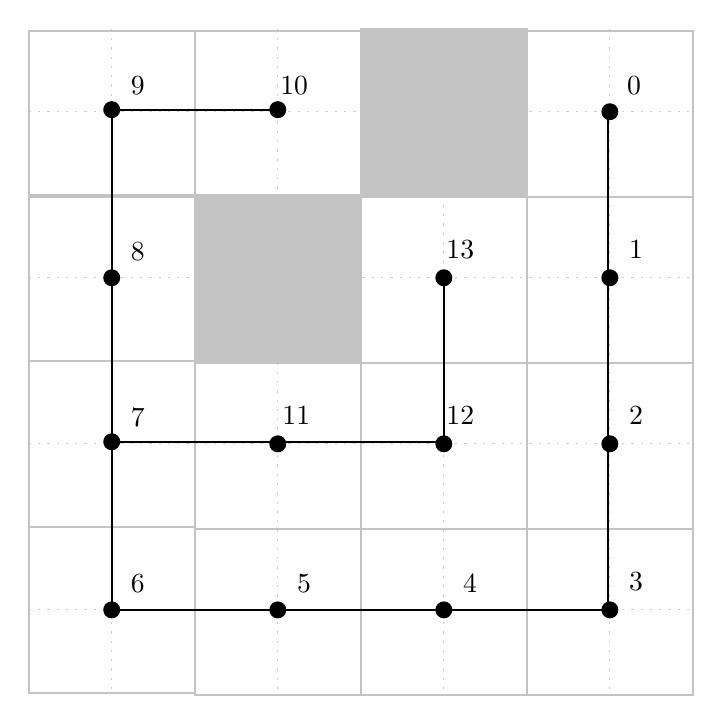
\begin{tikzpicture}[x=0.75pt,y=0.75pt,yscale=-1,xscale=1]
		%uncomment if require: \path (0,487); %set diagram left start at 0, and has height of 487
		
		%Straight Lines [id:da07078059737294629] 
		\draw [color={rgb, 255:red, 195; green, 195; blue, 195 }  ,draw opacity=0.8 ] [dash pattern={on 0.84pt off 2.51pt}]  (160,20) -- (160,340) ;
		%Straight Lines [id:da917458971819372] 
		\draw [color={rgb, 255:red, 195; green, 195; blue, 195 }  ,draw opacity=0.8 ] [dash pattern={on 0.84pt off 2.51pt}]  (240,20) -- (240,340) ;
		%Straight Lines [id:da8412450773677167] 
		\draw [color={rgb, 255:red, 195; green, 195; blue, 195 }  ,draw opacity=0.8 ] [dash pattern={on 0.84pt off 2.51pt}]  (320,20) -- (320,340) ;
		%Straight Lines [id:da3101903735332392] 
		\draw [color={rgb, 255:red, 195; green, 195; blue, 195 }  ,draw opacity=0.8 ] [dash pattern={on 0.84pt off 2.51pt}]  (400,20) -- (400,340) ;
		%Straight Lines [id:da43752561891339337] 
		\draw [color={rgb, 255:red, 195; green, 195; blue, 195 }  ,draw opacity=0.8 ] [dash pattern={on 0.84pt off 2.51pt}]  (120,60) -- (440,60) ;
		%Straight Lines [id:da21568167599612686] 
		\draw [color={rgb, 255:red, 195; green, 195; blue, 195 }  ,draw opacity=0.8 ] [dash pattern={on 0.84pt off 2.51pt}]  (120,140) -- (440,140) ;
		%Straight Lines [id:da9351274558937845] 
		\draw [color={rgb, 255:red, 195; green, 195; blue, 195 }  ,draw opacity=0.8 ] [dash pattern={on 0.84pt off 2.51pt}]  (120,220) -- (440,220) ;
		%Straight Lines [id:da8497636326794216] 
		\draw [color={rgb, 255:red, 195; green, 195; blue, 195 }  ,draw opacity=0.8 ] [dash pattern={on 0.84pt off 2.51pt}]  (120,300) -- (440,300) ;
		
		%Shape: Rectangle [id:dp7512840321055914] 
		\draw  [color={rgb, 255:red, 195; green, 195; blue, 195 }  ,draw opacity=1 ][line width=0.75]  (360,21) -- (440,21) -- (440,101) -- (360,101) -- cycle ;
		%Shape: Rectangle [id:dp08998875837998588] 
		\draw  [color={rgb, 255:red, 195; green, 195; blue, 195 }  ,draw opacity=1 ][line width=0.75]  (360,101) -- (440,101) -- (440,181) -- (360,181) -- cycle ;
		%Shape: Rectangle [id:dp0951355467677828] 
		\draw  [color={rgb, 255:red, 195; green, 195; blue, 195 }  ,draw opacity=1 ][line width=0.75]  (360,181) -- (440,181) -- (440,261) -- (360,261) -- cycle ;
		%Shape: Rectangle [id:dp7521114125139936] 
		\draw  [color={rgb, 255:red, 195; green, 195; blue, 195 }  ,draw opacity=1 ][line width=0.75]  (360,261) -- (440,261) -- (440,341) -- (360,341) -- cycle ;
		%Shape: Rectangle [id:dp7559961198567777] 
		\draw  [color={rgb, 255:red, 195; green, 195; blue, 195 }  ,draw opacity=1 ][line width=0.75]  (280,101) -- (360,101) -- (360,181) -- (280,181) -- cycle ;
		%Shape: Rectangle [id:dp8869961360769938] 
		\draw  [color={rgb, 255:red, 195; green, 195; blue, 195 }  ,draw opacity=1 ][line width=0.75]  (280,181) -- (360,181) -- (360,261) -- (280,261) -- cycle ;
		%Shape: Rectangle [id:dp5037977259529054] 
		\draw  [color={rgb, 255:red, 195; green, 195; blue, 195 }  ,draw opacity=1 ][line width=0.75]  (280,261) -- (360,261) -- (360,341) -- (280,341) -- cycle ;
		%Shape: Rectangle [id:dp773885446585411] 
		\draw  [color={rgb, 255:red, 195; green, 195; blue, 195 }  ,draw opacity=1 ][line width=0.75]  (200,21) -- (280,21) -- (280,101) -- (200,101) -- cycle ;
		%Shape: Rectangle [id:dp2052220638960709] 
		\draw  [color={rgb, 255:red, 195; green, 195; blue, 195 }  ,draw opacity=1 ][line width=0.75]  (120,21) -- (200,21) -- (200,101) -- (120,101) -- cycle ;
		%Shape: Rectangle [id:dp7105833624892055] 
		\draw  [color={rgb, 255:red, 195; green, 195; blue, 195 }  ,draw opacity=1 ][line width=0.75]  (120,100) -- (200,100) -- (200,180) -- (120,180) -- cycle ;
		%Shape: Rectangle [id:dp25180360725760975] 
		\draw  [color={rgb, 255:red, 195; green, 195; blue, 195 }  ,draw opacity=1 ][line width=0.75]  (120,180) -- (200,180) -- (200,260) -- (120,260) -- cycle ;
		%Shape: Rectangle [id:dp8614444924044413] 
		\draw  [color={rgb, 255:red, 195; green, 195; blue, 195 }  ,draw opacity=1 ][line width=0.75]  (120,260) -- (200,260) -- (200,340) -- (120,340) -- cycle ;
		%Shape: Rectangle [id:dp8378559698110666] 
		\draw  [color={rgb, 255:red, 195; green, 195; blue, 195 }  ,draw opacity=1 ][line width=0.75]  (200,181) -- (280,181) -- (280,261) -- (200,261) -- cycle ;
		%Shape: Rectangle [id:dp8380708528890195] 
		\draw  [color={rgb, 255:red, 195; green, 195; blue, 195 }  ,draw opacity=1 ][line width=0.75]  (200,261) -- (280,261) -- (280,341) -- (200,341) -- cycle ;
		
		%Straight Lines [id:da1979706309085778] 
		\draw [color={rgb, 255:red, 0; green, 0; blue, 0 }  ,draw opacity=1 ][line width=0.75]    (160,299) -- (160,59) ;
		%Shape: Rectangle [id:dp7251933800186736] 
		\draw  [color={rgb, 255:red, 195; green, 195; blue, 195 }  ,draw opacity=1 ][fill={rgb, 255:red, 195; green, 195; blue, 195 }  ,fill opacity=1 ][line width=0.75]  (280,20) -- (360,20) -- (360,100) -- (280,100) -- cycle ;
		%Shape: Rectangle [id:dp1925911620328833] 
		\draw  [color={rgb, 255:red, 195; green, 195; blue, 195 }  ,draw opacity=1 ][fill={rgb, 255:red, 195; green, 195; blue, 195 }  ,fill opacity=1 ][line width=0.75]  (200,100) -- (280,100) -- (280,180) -- (200,180) -- cycle ;
		%Straight Lines [id:da0581482096059478] 
		\draw [color={rgb, 255:red, 0; green, 0; blue, 0 }  ,draw opacity=1 ][line width=0.75]    (160,300) -- (400,300) ;
		%Straight Lines [id:da8084405416238001] 
		\draw [color={rgb, 255:red, 0; green, 0; blue, 0 }  ,draw opacity=1 ][line width=0.75]    (160,59) -- (240,59) ;
		%Straight Lines [id:da41325892147339616] 
		\draw [color={rgb, 255:red, 0; green, 0; blue, 0 }  ,draw opacity=1 ][fill={rgb, 255:red, 155; green, 155; blue, 155 }  ,fill opacity=1 ][line width=0.75]    (160,219) -- (320,219) ;
		%Straight Lines [id:da0985686119799063] 
		\draw [color={rgb, 255:red, 0; green, 0; blue, 0 }  ,draw opacity=1 ][line width=0.75]    (320,220) -- (320,140) ;
		%Straight Lines [id:da3298203658421879] 
		\draw [color={rgb, 255:red, 0; green, 0; blue, 0 }  ,draw opacity=1 ][line width=0.75]    (399,300) -- (399,60) ;
		%Shape: Circle [id:dp41582492626714096] 
		\draw  [color={rgb, 255:red, 0; green, 0; blue, 0 }  ,draw opacity=1 ][fill={rgb, 255:red, 0; green, 0; blue, 0 }  ,fill opacity=1 ] (236.19,59) .. controls (236.19,56.89) and (237.89,55.19) .. (240,55.19) .. controls (242.11,55.19) and (243.81,56.89) .. (243.81,59) .. controls (243.81,61.11) and (242.11,62.81) .. (240,62.81) .. controls (237.89,62.81) and (236.19,61.11) .. (236.19,59) -- cycle ;
		%Shape: Circle [id:dp5558894380647834] 
		\draw  [color={rgb, 255:red, 0; green, 0; blue, 0 }  ,draw opacity=1 ][fill={rgb, 255:red, 0; green, 0; blue, 0 }  ,fill opacity=1 ] (156.19,59) .. controls (156.19,56.89) and (157.89,55.19) .. (160,55.19) .. controls (162.11,55.19) and (163.81,56.89) .. (163.81,59) .. controls (163.81,61.11) and (162.11,62.81) .. (160,62.81) .. controls (157.89,62.81) and (156.19,61.11) .. (156.19,59) -- cycle ;
		%Shape: Circle [id:dp8351577385814617] 
		\draw  [color={rgb, 255:red, 0; green, 0; blue, 0 }  ,draw opacity=1 ][fill={rgb, 255:red, 0; green, 0; blue, 0 }  ,fill opacity=1 ] (396.19,60) .. controls (396.19,57.89) and (397.89,56.19) .. (400,56.19) .. controls (402.11,56.19) and (403.81,57.89) .. (403.81,60) .. controls (403.81,62.11) and (402.11,63.81) .. (400,63.81) .. controls (397.89,63.81) and (396.19,62.11) .. (396.19,60) -- cycle ;
		%Shape: Circle [id:dp7940426606232267] 
		\draw  [color={rgb, 255:red, 0; green, 0; blue, 0 }  ,draw opacity=1 ][fill={rgb, 255:red, 0; green, 0; blue, 0 }  ,fill opacity=1 ] (316.19,140) .. controls (316.19,137.89) and (317.89,136.19) .. (320,136.19) .. controls (322.11,136.19) and (323.81,137.89) .. (323.81,140) .. controls (323.81,142.11) and (322.11,143.81) .. (320,143.81) .. controls (317.89,143.81) and (316.19,142.11) .. (316.19,140) -- cycle ;
		%Shape: Circle [id:dp04520481160188616] 
		\draw  [color={rgb, 255:red, 0; green, 0; blue, 0 }  ,draw opacity=1 ][fill={rgb, 255:red, 0; green, 0; blue, 0 }  ,fill opacity=1 ] (316.19,220) .. controls (316.19,217.89) and (317.89,216.19) .. (320,216.19) .. controls (322.11,216.19) and (323.81,217.89) .. (323.81,220) .. controls (323.81,222.11) and (322.11,223.81) .. (320,223.81) .. controls (317.89,223.81) and (316.19,222.11) .. (316.19,220) -- cycle ;
		%Shape: Circle [id:dp5073699623939971] 
		\draw  [color={rgb, 255:red, 0; green, 0; blue, 0 }  ,draw opacity=1 ][fill={rgb, 255:red, 0; green, 0; blue, 0 }  ,fill opacity=1 ] (236.19,220) .. controls (236.19,217.89) and (237.89,216.19) .. (240,216.19) .. controls (242.11,216.19) and (243.81,217.89) .. (243.81,220) .. controls (243.81,222.11) and (242.11,223.81) .. (240,223.81) .. controls (237.89,223.81) and (236.19,222.11) .. (236.19,220) -- cycle ;
		%Shape: Circle [id:dp2213240590117067] 
		\draw  [color={rgb, 255:red, 0; green, 0; blue, 0 }  ,draw opacity=1 ][fill={rgb, 255:red, 0; green, 0; blue, 0 }  ,fill opacity=1 ] (156.19,219) .. controls (156.19,216.89) and (157.89,215.19) .. (160,215.19) .. controls (162.11,215.19) and (163.81,216.89) .. (163.81,219) .. controls (163.81,221.11) and (162.11,222.81) .. (160,222.81) .. controls (157.89,222.81) and (156.19,221.11) .. (156.19,219) -- cycle ;
		%Shape: Circle [id:dp979294341687238] 
		\draw  [color={rgb, 255:red, 0; green, 0; blue, 0 }  ,draw opacity=1 ][fill={rgb, 255:red, 0; green, 0; blue, 0 }  ,fill opacity=1 ] (156.19,140) .. controls (156.19,137.89) and (157.89,136.19) .. (160,136.19) .. controls (162.11,136.19) and (163.81,137.89) .. (163.81,140) .. controls (163.81,142.11) and (162.11,143.81) .. (160,143.81) .. controls (157.89,143.81) and (156.19,142.11) .. (156.19,140) -- cycle ;
		%Shape: Circle [id:dp14676659616041077] 
		\draw  [color={rgb, 255:red, 0; green, 0; blue, 0 }  ,draw opacity=1 ][fill={rgb, 255:red, 0; green, 0; blue, 0 }  ,fill opacity=1 ] (396.19,140) .. controls (396.19,137.89) and (397.89,136.19) .. (400,136.19) .. controls (402.11,136.19) and (403.81,137.89) .. (403.81,140) .. controls (403.81,142.11) and (402.11,143.81) .. (400,143.81) .. controls (397.89,143.81) and (396.19,142.11) .. (396.19,140) -- cycle ;
		%Shape: Circle [id:dp19334338983125243] 
		\draw  [color={rgb, 255:red, 0; green, 0; blue, 0 }  ,draw opacity=1 ][fill={rgb, 255:red, 0; green, 0; blue, 0 }  ,fill opacity=1 ] (396.19,220) .. controls (396.19,217.89) and (397.89,216.19) .. (400,216.19) .. controls (402.11,216.19) and (403.81,217.89) .. (403.81,220) .. controls (403.81,222.11) and (402.11,223.81) .. (400,223.81) .. controls (397.89,223.81) and (396.19,222.11) .. (396.19,220) -- cycle ;
		%Shape: Circle [id:dp5263269612866854] 
		\draw  [color={rgb, 255:red, 0; green, 0; blue, 0 }  ,draw opacity=1 ][fill={rgb, 255:red, 0; green, 0; blue, 0 }  ,fill opacity=1 ] (396.19,300) .. controls (396.19,297.89) and (397.89,296.19) .. (400,296.19) .. controls (402.11,296.19) and (403.81,297.89) .. (403.81,300) .. controls (403.81,302.11) and (402.11,303.81) .. (400,303.81) .. controls (397.89,303.81) and (396.19,302.11) .. (396.19,300) -- cycle ;
		%Shape: Circle [id:dp41455563786620653] 
		\draw  [color={rgb, 255:red, 0; green, 0; blue, 0 }  ,draw opacity=1 ][fill={rgb, 255:red, 0; green, 0; blue, 0 }  ,fill opacity=1 ] (316.19,300) .. controls (316.19,297.89) and (317.89,296.19) .. (320,296.19) .. controls (322.11,296.19) and (323.81,297.89) .. (323.81,300) .. controls (323.81,302.11) and (322.11,303.81) .. (320,303.81) .. controls (317.89,303.81) and (316.19,302.11) .. (316.19,300) -- cycle ;
		%Shape: Circle [id:dp9746259257783465] 
		\draw  [color={rgb, 255:red, 0; green, 0; blue, 0 }  ,draw opacity=1 ][fill={rgb, 255:red, 0; green, 0; blue, 0 }  ,fill opacity=1 ] (236.19,300) .. controls (236.19,297.89) and (237.89,296.19) .. (240,296.19) .. controls (242.11,296.19) and (243.81,297.89) .. (243.81,300) .. controls (243.81,302.11) and (242.11,303.81) .. (240,303.81) .. controls (237.89,303.81) and (236.19,302.11) .. (236.19,300) -- cycle ;
		%Shape: Circle [id:dp5753636930291428] 
		\draw  [color={rgb, 255:red, 0; green, 0; blue, 0 }  ,draw opacity=1 ][fill={rgb, 255:red, 0; green, 0; blue, 0 }  ,fill opacity=1 ] (156.19,300) .. controls (156.19,297.89) and (157.89,296.19) .. (160,296.19) .. controls (162.11,296.19) and (163.81,297.89) .. (163.81,300) .. controls (163.81,302.11) and (162.11,303.81) .. (160,303.81) .. controls (157.89,303.81) and (156.19,302.11) .. (156.19,300) -- cycle ;
		
		% Text Node
		\draw (407,42) node [anchor=north west][inner sep=0.75pt]   [align=left] {0};
		% Text Node
		\draw (408,121) node [anchor=north west][inner sep=0.75pt]   [align=left] {1};
		% Text Node
		\draw (408,201) node [anchor=north west][inner sep=0.75pt]   [align=left] {2};
		% Text Node
		\draw (408,281) node [anchor=north west][inner sep=0.75pt]   [align=left] {3};
		% Text Node
		\draw (328,282) node [anchor=north west][inner sep=0.75pt]   [align=left] {4};
		% Text Node
		\draw (248,282) node [anchor=north west][inner sep=0.75pt]   [align=left] {5};
		% Text Node
		\draw (168,282) node [anchor=north west][inner sep=0.75pt]   [align=left] {6};
		% Text Node
		\draw (168,202) node [anchor=north west][inner sep=0.75pt]   [align=left] {7};
		% Text Node
		\draw (168,122) node [anchor=north west][inner sep=0.75pt]   [align=left] {8};
		% Text Node
		\draw (168,42) node [anchor=north west][inner sep=0.75pt]   [align=left] {9};
		% Text Node
		\draw (240,42) node [anchor=north west][inner sep=0.75pt]   [align=left] {10};
		% Text Node
		\draw (241,201) node [anchor=north west][inner sep=0.75pt]   [align=left] {11};
		% Text Node
		\draw (320,201) node [anchor=north west][inner sep=0.75pt]   [align=left] {12};
		% Text Node
		\draw (320,121) node [anchor=north west][inner sep=0.75pt]   [align=left] {13};
		
		
	\end{tikzpicture}
	\caption{Figure showing a spanning tree generated for a four-by-four environment grid}
	\label{fig:grid-st}
\end{figure}

\begin{figure}[h!]
	\centering
	\tikzset{every picture/.style={line width=0.75pt}} %set default line width to 0.75pt        
	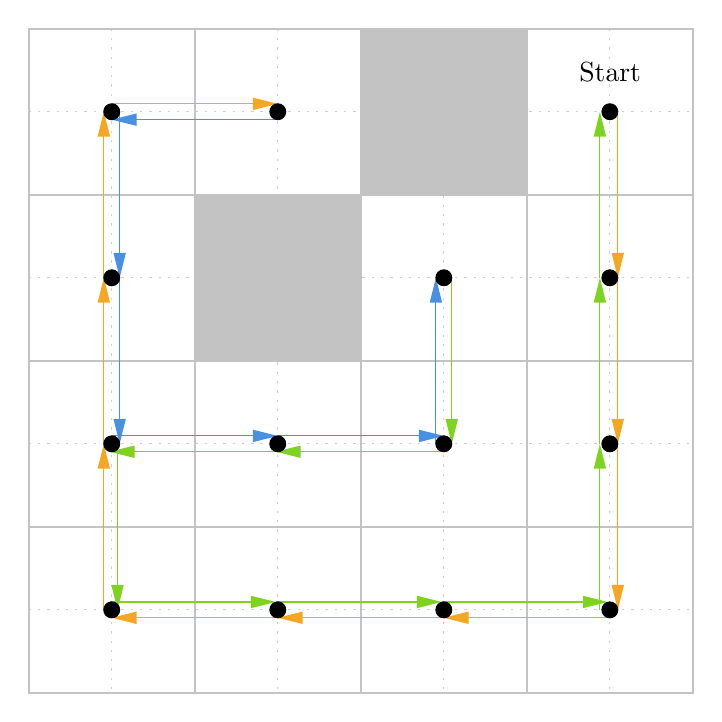
\begin{tikzpicture}[x=0.75pt,y=0.75pt,yscale=-1,xscale=1]
		%uncomment if require: \path (0,487); %set diagram left start at 0, and has height of 487
		
		%Straight Lines [id:da3977750045093258] 
		\draw [color={rgb, 255:red, 195; green, 195; blue, 195 }  ,draw opacity=0.8 ] [dash pattern={on 0.84pt off 2.51pt}]  (160,20) -- (160,340) ;
		%Straight Lines [id:da07618883915401731] 
		\draw [color={rgb, 255:red, 195; green, 195; blue, 195 }  ,draw opacity=0.8 ] [dash pattern={on 0.84pt off 2.51pt}]  (240,20) -- (240,340) ;
		%Straight Lines [id:da06600432409341517] 
		\draw [color={rgb, 255:red, 195; green, 195; blue, 195 }  ,draw opacity=0.8 ] [dash pattern={on 0.84pt off 2.51pt}]  (320,20) -- (320,340) ;
		%Straight Lines [id:da5290784258779333] 
		\draw [color={rgb, 255:red, 195; green, 195; blue, 195 }  ,draw opacity=0.8 ] [dash pattern={on 0.84pt off 2.51pt}]  (400,20) -- (400,340) ;
		%Straight Lines [id:da9833595064287617] 
		\draw [color={rgb, 255:red, 195; green, 195; blue, 195 }  ,draw opacity=0.8 ] [dash pattern={on 0.84pt off 2.51pt}]  (120,60) -- (440,60) ;
		%Straight Lines [id:da520432231001738] 
		\draw [color={rgb, 255:red, 195; green, 195; blue, 195 }  ,draw opacity=0.8 ] [dash pattern={on 0.84pt off 2.51pt}]  (120,140) -- (440,140) ;
		%Straight Lines [id:da6002867106183594] 
		\draw [color={rgb, 255:red, 195; green, 195; blue, 195 }  ,draw opacity=0.8 ] [dash pattern={on 0.84pt off 2.51pt}]  (120,220) -- (440,220) ;
		%Straight Lines [id:da9782745721301296] 
		\draw [color={rgb, 255:red, 195; green, 195; blue, 195 }  ,draw opacity=0.8 ] [dash pattern={on 0.84pt off 2.51pt}]  (120,300) -- (440,300) ;
		
		%Shape: Rectangle [id:dp5898184612923194] 
		\draw  [color={rgb, 255:red, 195; green, 195; blue, 195 }  ,draw opacity=1 ][line width=0.75]  (360,20) -- (440,20) -- (440,100) -- (360,100) -- cycle ;
		%Shape: Rectangle [id:dp48862096625716034] 
		\draw  [color={rgb, 255:red, 195; green, 195; blue, 195 }  ,draw opacity=1 ][line width=0.75]  (360,100) -- (440,100) -- (440,180) -- (360,180) -- cycle ;
		%Shape: Rectangle [id:dp3755148108063808] 
		\draw  [color={rgb, 255:red, 195; green, 195; blue, 195 }  ,draw opacity=1 ][line width=0.75]  (360,180) -- (440,180) -- (440,260) -- (360,260) -- cycle ;
		%Shape: Rectangle [id:dp9473736210218475] 
		\draw  [color={rgb, 255:red, 195; green, 195; blue, 195 }  ,draw opacity=1 ][line width=0.75]  (360,260) -- (440,260) -- (440,340) -- (360,340) -- cycle ;
		%Shape: Rectangle [id:dp12436408430349899] 
		\draw  [color={rgb, 255:red, 195; green, 195; blue, 195 }  ,draw opacity=1 ][line width=0.75]  (280,100) -- (360,100) -- (360,180) -- (280,180) -- cycle ;
		%Shape: Rectangle [id:dp43828113255227175] 
		\draw  [color={rgb, 255:red, 195; green, 195; blue, 195 }  ,draw opacity=1 ][line width=0.75]  (280,180) -- (360,180) -- (360,260) -- (280,260) -- cycle ;
		%Shape: Rectangle [id:dp7405502584040733] 
		\draw  [color={rgb, 255:red, 195; green, 195; blue, 195 }  ,draw opacity=1 ][line width=0.75]  (280,260) -- (360,260) -- (360,340) -- (280,340) -- cycle ;
		%Shape: Rectangle [id:dp05296394236381641] 
		\draw  [color={rgb, 255:red, 195; green, 195; blue, 195 }  ,draw opacity=1 ][line width=0.75]  (120,20) -- (200,20) -- (200,100) -- (120,100) -- cycle ;
		%Shape: Rectangle [id:dp6150857421701121] 
		\draw  [color={rgb, 255:red, 195; green, 195; blue, 195 }  ,draw opacity=1 ][line width=0.75]  (120,100) -- (200,100) -- (200,180) -- (120,180) -- cycle ;
		%Shape: Rectangle [id:dp5861189397744904] 
		\draw  [color={rgb, 255:red, 195; green, 195; blue, 195 }  ,draw opacity=1 ][line width=0.75]  (120,180) -- (200,180) -- (200,260) -- (120,260) -- cycle ;
		%Shape: Rectangle [id:dp8672396938760043] 
		\draw  [color={rgb, 255:red, 195; green, 195; blue, 195 }  ,draw opacity=1 ][line width=0.75]  (120,260) -- (200,260) -- (200,340) -- (120,340) -- cycle ;
		%Shape: Rectangle [id:dp32997979058045] 
		\draw  [color={rgb, 255:red, 195; green, 195; blue, 195 }  ,draw opacity=1 ][line width=0.75]  (200,180) -- (280,180) -- (280,260) -- (200,260) -- cycle ;
		%Shape: Rectangle [id:dp6083880745681156] 
		\draw  [color={rgb, 255:red, 195; green, 195; blue, 195 }  ,draw opacity=1 ][line width=0.75]  (200,260) -- (280,260) -- (280,340) -- (200,340) -- cycle ;
		
		%Shape: Rectangle [id:dp6989257767580808] 
		\draw  [color={rgb, 255:red, 195; green, 195; blue, 195 }  ,draw opacity=1 ][line width=0.75]  (200,20) -- (280,20) -- (280,100) -- (200,100) -- cycle ;
		
		%Shape: Rectangle [id:dp3496282639540844] 
		\draw  [color={rgb, 255:red, 195; green, 195; blue, 195 }  ,draw opacity=1 ][fill={rgb, 255:red, 195; green, 195; blue, 195 }  ,fill opacity=1 ][line width=0.75]  (280,20) -- (360,20) -- (360,100) -- (280,100) -- cycle ;
		%Shape: Rectangle [id:dp1101274608527989] 
		\draw  [color={rgb, 255:red, 195; green, 195; blue, 195 }  ,draw opacity=1 ][fill={rgb, 255:red, 195; green, 195; blue, 195 }  ,fill opacity=1 ][line width=0.75]  (200,100) -- (280,100) -- (280,180) -- (200,180) -- cycle ;
		%Straight Lines [id:da7109877053031188] 
		\draw [color={rgb, 255:red, 245; green, 166; blue, 35 }  ,draw opacity=1 ]   (403.81,60) -- (403.81,138) ;
		\draw [shift={(403.81,140)}, rotate = 270] [fill={rgb, 255:red, 245; green, 166; blue, 35 }  ,fill opacity=1 ][line width=0.08]  [draw opacity=0] (12,-3) -- (0,0) -- (12,3) -- cycle    ;
		%Straight Lines [id:da26602598944672584] 
		\draw [color={rgb, 255:red, 126; green, 211; blue, 33 }  ,draw opacity=1 ]   (395.19,140) -- (395.19,62) ;
		\draw [shift={(395.19,60)}, rotate = 450] [fill={rgb, 255:red, 126; green, 211; blue, 33 }  ,fill opacity=1 ][line width=0.08]  [draw opacity=0] (12,-3) -- (0,0) -- (12,3) -- cycle    ;
		%Straight Lines [id:da02914591351940765] 
		\draw [color={rgb, 255:red, 126; green, 211; blue, 33 }  ,draw opacity=1 ]   (395.19,220) -- (395.19,142) ;
		\draw [shift={(395.19,140)}, rotate = 450] [fill={rgb, 255:red, 126; green, 211; blue, 33 }  ,fill opacity=1 ][line width=0.08]  [draw opacity=0] (12,-3) -- (0,0) -- (12,3) -- cycle    ;
		%Straight Lines [id:da39308513285178037] 
		\draw [color={rgb, 255:red, 245; green, 166; blue, 35 }  ,draw opacity=1 ]   (403.81,140) -- (403.81,218) ;
		\draw [shift={(403.81,220)}, rotate = 270] [fill={rgb, 255:red, 245; green, 166; blue, 35 }  ,fill opacity=1 ][line width=0.08]  [draw opacity=0] (12,-3) -- (0,0) -- (12,3) -- cycle    ;
		%Straight Lines [id:da5373248798431745] 
		\draw [color={rgb, 255:red, 245; green, 166; blue, 35 }  ,draw opacity=1 ]   (403.81,220) -- (403.81,298) ;
		\draw [shift={(403.81,300)}, rotate = 270] [fill={rgb, 255:red, 245; green, 166; blue, 35 }  ,fill opacity=1 ][line width=0.08]  [draw opacity=0] (12,-3) -- (0,0) -- (12,3) -- cycle    ;
		%Straight Lines [id:da6507397451478356] 
		\draw [color={rgb, 255:red, 126; green, 211; blue, 33 }  ,draw opacity=1 ]   (395.19,300) -- (395.19,222) ;
		\draw [shift={(395.19,220)}, rotate = 450] [fill={rgb, 255:red, 126; green, 211; blue, 33 }  ,fill opacity=1 ][line width=0.08]  [draw opacity=0] (12,-3) -- (0,0) -- (12,3) -- cycle    ;
		%Straight Lines [id:da4490944583331955] 
		\draw [color={rgb, 255:red, 245; green, 166; blue, 35 }  ,draw opacity=1 ]   (400,303.81) -- (322,303.81) ;
		\draw [shift={(320,303.81)}, rotate = 360] [fill={rgb, 255:red, 245; green, 166; blue, 35 }  ,fill opacity=1 ][line width=0.08]  [draw opacity=0] (12,-3) -- (0,0) -- (12,3) -- cycle    ;
		%Straight Lines [id:da771333880279802] 
		\draw [color={rgb, 255:red, 245; green, 166; blue, 35 }  ,draw opacity=1 ]   (320,303.81) -- (242,303.81) ;
		\draw [shift={(240,303.81)}, rotate = 360] [fill={rgb, 255:red, 245; green, 166; blue, 35 }  ,fill opacity=1 ][line width=0.08]  [draw opacity=0] (12,-3) -- (0,0) -- (12,3) -- cycle    ;
		%Straight Lines [id:da0915527602751669] 
		\draw [color={rgb, 255:red, 245; green, 166; blue, 35 }  ,draw opacity=1 ]   (240,303.81) -- (162,303.81) ;
		\draw [shift={(160,303.81)}, rotate = 360] [fill={rgb, 255:red, 245; green, 166; blue, 35 }  ,fill opacity=1 ][line width=0.08]  [draw opacity=0] (12,-3) -- (0,0) -- (12,3) -- cycle    ;
		%Straight Lines [id:da8183550519262464] 
		\draw [color={rgb, 255:red, 126; green, 211; blue, 33 }  ,draw opacity=1 ]   (319,296.19) -- (397,296.19) ;
		\draw [shift={(399,296.19)}, rotate = 180] [fill={rgb, 255:red, 126; green, 211; blue, 33 }  ,fill opacity=1 ][line width=0.08]  [draw opacity=0] (12,-3) -- (0,0) -- (12,3) -- cycle    ;
		%Straight Lines [id:da270699769832347] 
		\draw [color={rgb, 255:red, 126; green, 211; blue, 33 }  ,draw opacity=1 ]   (239,296.19) -- (317,296.19) ;
		\draw [shift={(319,296.19)}, rotate = 180] [fill={rgb, 255:red, 126; green, 211; blue, 33 }  ,fill opacity=1 ][line width=0.08]  [draw opacity=0] (12,-3) -- (0,0) -- (12,3) -- cycle    ;
		%Straight Lines [id:da5296508036432168] 
		\draw [color={rgb, 255:red, 126; green, 211; blue, 33 }  ,draw opacity=1 ]   (159,296.19) -- (237,296.19) ;
		\draw [shift={(239,296.19)}, rotate = 180] [fill={rgb, 255:red, 126; green, 211; blue, 33 }  ,fill opacity=1 ][line width=0.08]  [draw opacity=0] (12,-3) -- (0,0) -- (12,3) -- cycle    ;
		%Straight Lines [id:da6152908850819139] 
		\draw [color={rgb, 255:red, 245; green, 166; blue, 35 }  ,draw opacity=1 ]   (156.19,300) -- (156.19,222) ;
		\draw [shift={(156.19,220)}, rotate = 450] [fill={rgb, 255:red, 245; green, 166; blue, 35 }  ,fill opacity=1 ][line width=0.08]  [draw opacity=0] (12,-3) -- (0,0) -- (12,3) -- cycle    ;
		%Straight Lines [id:da4869759720464193] 
		\draw [color={rgb, 255:red, 245; green, 166; blue, 35 }  ,draw opacity=1 ]   (160,56.19) -- (238,56.19) ;
		\draw [shift={(240,56.19)}, rotate = 180] [fill={rgb, 255:red, 245; green, 166; blue, 35 }  ,fill opacity=1 ][line width=0.08]  [draw opacity=0] (12,-3) -- (0,0) -- (12,3) -- cycle    ;
		%Straight Lines [id:da41392688240238984] 
		\draw [color={rgb, 255:red, 74; green, 144; blue, 226 }  ,draw opacity=1 ]   (240,63.81) -- (162,63.81) ;
		\draw [shift={(160,63.81)}, rotate = 360] [fill={rgb, 255:red, 74; green, 144; blue, 226 }  ,fill opacity=1 ][line width=0.08]  [draw opacity=0] (12,-3) -- (0,0) -- (12,3) -- cycle    ;
		%Straight Lines [id:da1371170506661339] 
		\draw [color={rgb, 255:red, 126; green, 211; blue, 33 }  ,draw opacity=1 ]   (162.81,220) -- (162.81,298) ;
		\draw [shift={(162.81,300)}, rotate = 270] [fill={rgb, 255:red, 126; green, 211; blue, 33 }  ,fill opacity=1 ][line width=0.08]  [draw opacity=0] (12,-3) -- (0,0) -- (12,3) -- cycle    ;
		%Straight Lines [id:da06913212613382202] 
		\draw [color={rgb, 255:red, 74; green, 144; blue, 226 }  ,draw opacity=1 ]   (160,216.19) -- (238,216.19) ;
		\draw [shift={(240,216.19)}, rotate = 180] [fill={rgb, 255:red, 74; green, 144; blue, 226 }  ,fill opacity=1 ][line width=0.08]  [draw opacity=0] (12,-3) -- (0,0) -- (12,3) -- cycle    ;
		%Straight Lines [id:da37746092338955006] 
		\draw [color={rgb, 255:red, 126; green, 211; blue, 33 }  ,draw opacity=1 ]   (239,223.81) -- (161,223.81) ;
		\draw [shift={(159,223.81)}, rotate = 360] [fill={rgb, 255:red, 126; green, 211; blue, 33 }  ,fill opacity=1 ][line width=0.08]  [draw opacity=0] (12,-3) -- (0,0) -- (12,3) -- cycle    ;
		%Straight Lines [id:da5502420093118436] 
		\draw [color={rgb, 255:red, 126; green, 211; blue, 33 }  ,draw opacity=1 ]   (319,223.81) -- (241,223.81) ;
		\draw [shift={(239,223.81)}, rotate = 360] [fill={rgb, 255:red, 126; green, 211; blue, 33 }  ,fill opacity=1 ][line width=0.08]  [draw opacity=0] (12,-3) -- (0,0) -- (12,3) -- cycle    ;
		%Straight Lines [id:da25223475086499536] 
		\draw [color={rgb, 255:red, 74; green, 144; blue, 226 }  ,draw opacity=1 ]   (240,216.19) -- (318,216.19) ;
		\draw [shift={(320,216.19)}, rotate = 180] [fill={rgb, 255:red, 74; green, 144; blue, 226 }  ,fill opacity=1 ][line width=0.08]  [draw opacity=0] (12,-3) -- (0,0) -- (12,3) -- cycle    ;
		%Straight Lines [id:da8200476146784395] 
		\draw [color={rgb, 255:red, 74; green, 144; blue, 226 }  ,draw opacity=1 ]   (316.19,220) -- (316.19,142) ;
		\draw [shift={(316.19,140)}, rotate = 450] [fill={rgb, 255:red, 74; green, 144; blue, 226 }  ,fill opacity=1 ][line width=0.08]  [draw opacity=0] (12,-3) -- (0,0) -- (12,3) -- cycle    ;
		%Straight Lines [id:da5178980162476476] 
		\draw [color={rgb, 255:red, 126; green, 211; blue, 33 }  ,draw opacity=1 ]   (323.81,140) -- (323.81,218) ;
		\draw [shift={(323.81,220)}, rotate = 270] [fill={rgb, 255:red, 126; green, 211; blue, 33 }  ,fill opacity=1 ][line width=0.08]  [draw opacity=0] (12,-3) -- (0,0) -- (12,3) -- cycle    ;
		%Straight Lines [id:da5994423368626156] 
		\draw [color={rgb, 255:red, 245; green, 166; blue, 35 }  ,draw opacity=1 ]   (156.19,220) -- (156.19,142) ;
		\draw [shift={(156.19,140)}, rotate = 450] [fill={rgb, 255:red, 245; green, 166; blue, 35 }  ,fill opacity=1 ][line width=0.08]  [draw opacity=0] (12,-3) -- (0,0) -- (12,3) -- cycle    ;
		%Straight Lines [id:da2748369034984963] 
		\draw [color={rgb, 255:red, 74; green, 144; blue, 226 }  ,draw opacity=1 ]   (163.81,140) -- (163.81,218) ;
		\draw [shift={(163.81,220)}, rotate = 270] [fill={rgb, 255:red, 74; green, 144; blue, 226 }  ,fill opacity=1 ][line width=0.08]  [draw opacity=0] (12,-3) -- (0,0) -- (12,3) -- cycle    ;
		%Straight Lines [id:da6753173854185068] 
		\draw [color={rgb, 255:red, 74; green, 144; blue, 226 }  ,draw opacity=1 ]   (163.81,60) -- (163.81,138) ;
		\draw [shift={(163.81,140)}, rotate = 270] [fill={rgb, 255:red, 74; green, 144; blue, 226 }  ,fill opacity=1 ][line width=0.08]  [draw opacity=0] (12,-3) -- (0,0) -- (12,3) -- cycle    ;
		%Straight Lines [id:da6119419475380783] 
		\draw [color={rgb, 255:red, 245; green, 166; blue, 35 }  ,draw opacity=1 ]   (156.19,140) -- (156.19,62) ;
		\draw [shift={(156.19,60)}, rotate = 450] [fill={rgb, 255:red, 245; green, 166; blue, 35 }  ,fill opacity=1 ][line width=0.08]  [draw opacity=0] (12,-3) -- (0,0) -- (12,3) -- cycle    ;
		%Shape: Circle [id:dp5879652604634542] 
		\draw  [color={rgb, 255:red, 0; green, 0; blue, 0 }  ,draw opacity=1 ][fill={rgb, 255:red, 0; green, 0; blue, 0 }  ,fill opacity=1 ] (236.19,60) .. controls (236.19,57.89) and (237.89,56.19) .. (240,56.19) .. controls (242.11,56.19) and (243.81,57.89) .. (243.81,60) .. controls (243.81,62.11) and (242.11,63.81) .. (240,63.81) .. controls (237.89,63.81) and (236.19,62.11) .. (236.19,60) -- cycle ;
		%Shape: Circle [id:dp818491645062577] 
		\draw  [color={rgb, 255:red, 0; green, 0; blue, 0 }  ,draw opacity=1 ][fill={rgb, 255:red, 0; green, 0; blue, 0 }  ,fill opacity=1 ] (156.19,60) .. controls (156.19,57.89) and (157.89,56.19) .. (160,56.19) .. controls (162.11,56.19) and (163.81,57.89) .. (163.81,60) .. controls (163.81,62.11) and (162.11,63.81) .. (160,63.81) .. controls (157.89,63.81) and (156.19,62.11) .. (156.19,60) -- cycle ;
		%Shape: Circle [id:dp16964786331372994] 
		\draw  [color={rgb, 255:red, 0; green, 0; blue, 0 }  ,draw opacity=1 ][fill={rgb, 255:red, 0; green, 0; blue, 0 }  ,fill opacity=1 ] (396.19,60) .. controls (396.19,57.89) and (397.89,56.19) .. (400,56.19) .. controls (402.11,56.19) and (403.81,57.89) .. (403.81,60) .. controls (403.81,62.11) and (402.11,63.81) .. (400,63.81) .. controls (397.89,63.81) and (396.19,62.11) .. (396.19,60) -- cycle ;
		%Shape: Circle [id:dp12685321021069051] 
		\draw  [color={rgb, 255:red, 0; green, 0; blue, 0 }  ,draw opacity=1 ][fill={rgb, 255:red, 0; green, 0; blue, 0 }  ,fill opacity=1 ] (316.19,140) .. controls (316.19,137.89) and (317.89,136.19) .. (320,136.19) .. controls (322.11,136.19) and (323.81,137.89) .. (323.81,140) .. controls (323.81,142.11) and (322.11,143.81) .. (320,143.81) .. controls (317.89,143.81) and (316.19,142.11) .. (316.19,140) -- cycle ;
		%Shape: Circle [id:dp14500238655020814] 
		\draw  [color={rgb, 255:red, 0; green, 0; blue, 0 }  ,draw opacity=1 ][fill={rgb, 255:red, 0; green, 0; blue, 0 }  ,fill opacity=1 ] (316.19,220) .. controls (316.19,217.89) and (317.89,216.19) .. (320,216.19) .. controls (322.11,216.19) and (323.81,217.89) .. (323.81,220) .. controls (323.81,222.11) and (322.11,223.81) .. (320,223.81) .. controls (317.89,223.81) and (316.19,222.11) .. (316.19,220) -- cycle ;
		%Shape: Circle [id:dp007101657201895817] 
		\draw  [color={rgb, 255:red, 0; green, 0; blue, 0 }  ,draw opacity=1 ][fill={rgb, 255:red, 0; green, 0; blue, 0 }  ,fill opacity=1 ] (236.19,220) .. controls (236.19,217.89) and (237.89,216.19) .. (240,216.19) .. controls (242.11,216.19) and (243.81,217.89) .. (243.81,220) .. controls (243.81,222.11) and (242.11,223.81) .. (240,223.81) .. controls (237.89,223.81) and (236.19,222.11) .. (236.19,220) -- cycle ;
		%Shape: Circle [id:dp19397915406266075] 
		\draw  [color={rgb, 255:red, 0; green, 0; blue, 0 }  ,draw opacity=1 ][fill={rgb, 255:red, 0; green, 0; blue, 0 }  ,fill opacity=1 ] (156.19,220) .. controls (156.19,217.89) and (157.89,216.19) .. (160,216.19) .. controls (162.11,216.19) and (163.81,217.89) .. (163.81,220) .. controls (163.81,222.11) and (162.11,223.81) .. (160,223.81) .. controls (157.89,223.81) and (156.19,222.11) .. (156.19,220) -- cycle ;
		%Shape: Circle [id:dp11650504808251783] 
		\draw  [color={rgb, 255:red, 0; green, 0; blue, 0 }  ,draw opacity=1 ][fill={rgb, 255:red, 0; green, 0; blue, 0 }  ,fill opacity=1 ] (156.19,140) .. controls (156.19,137.89) and (157.89,136.19) .. (160,136.19) .. controls (162.11,136.19) and (163.81,137.89) .. (163.81,140) .. controls (163.81,142.11) and (162.11,143.81) .. (160,143.81) .. controls (157.89,143.81) and (156.19,142.11) .. (156.19,140) -- cycle ;
		%Shape: Circle [id:dp14621496623583385] 
		\draw  [color={rgb, 255:red, 0; green, 0; blue, 0 }  ,draw opacity=1 ][fill={rgb, 255:red, 0; green, 0; blue, 0 }  ,fill opacity=1 ] (396.19,140) .. controls (396.19,137.89) and (397.89,136.19) .. (400,136.19) .. controls (402.11,136.19) and (403.81,137.89) .. (403.81,140) .. controls (403.81,142.11) and (402.11,143.81) .. (400,143.81) .. controls (397.89,143.81) and (396.19,142.11) .. (396.19,140) -- cycle ;
		%Shape: Circle [id:dp4178077365658106] 
		\draw  [color={rgb, 255:red, 0; green, 0; blue, 0 }  ,draw opacity=1 ][fill={rgb, 255:red, 0; green, 0; blue, 0 }  ,fill opacity=1 ] (396.19,220) .. controls (396.19,217.89) and (397.89,216.19) .. (400,216.19) .. controls (402.11,216.19) and (403.81,217.89) .. (403.81,220) .. controls (403.81,222.11) and (402.11,223.81) .. (400,223.81) .. controls (397.89,223.81) and (396.19,222.11) .. (396.19,220) -- cycle ;
		%Shape: Circle [id:dp5805338448968826] 
		\draw  [color={rgb, 255:red, 0; green, 0; blue, 0 }  ,draw opacity=1 ][fill={rgb, 255:red, 0; green, 0; blue, 0 }  ,fill opacity=1 ] (396.19,300) .. controls (396.19,297.89) and (397.89,296.19) .. (400,296.19) .. controls (402.11,296.19) and (403.81,297.89) .. (403.81,300) .. controls (403.81,302.11) and (402.11,303.81) .. (400,303.81) .. controls (397.89,303.81) and (396.19,302.11) .. (396.19,300) -- cycle ;
		%Shape: Circle [id:dp40812749698644635] 
		\draw  [color={rgb, 255:red, 0; green, 0; blue, 0 }  ,draw opacity=1 ][fill={rgb, 255:red, 0; green, 0; blue, 0 }  ,fill opacity=1 ] (316.19,300) .. controls (316.19,297.89) and (317.89,296.19) .. (320,296.19) .. controls (322.11,296.19) and (323.81,297.89) .. (323.81,300) .. controls (323.81,302.11) and (322.11,303.81) .. (320,303.81) .. controls (317.89,303.81) and (316.19,302.11) .. (316.19,300) -- cycle ;
		%Shape: Circle [id:dp6552313991625613] 
		\draw  [color={rgb, 255:red, 0; green, 0; blue, 0 }  ,draw opacity=1 ][fill={rgb, 255:red, 0; green, 0; blue, 0 }  ,fill opacity=1 ] (236.19,300) .. controls (236.19,297.89) and (237.89,296.19) .. (240,296.19) .. controls (242.11,296.19) and (243.81,297.89) .. (243.81,300) .. controls (243.81,302.11) and (242.11,303.81) .. (240,303.81) .. controls (237.89,303.81) and (236.19,302.11) .. (236.19,300) -- cycle ;
		%Shape: Circle [id:dp7003315075103178] 
		\draw  [color={rgb, 255:red, 0; green, 0; blue, 0 }  ,draw opacity=1 ][fill={rgb, 255:red, 0; green, 0; blue, 0 }  ,fill opacity=1 ] (156.19,300) .. controls (156.19,297.89) and (157.89,296.19) .. (160,296.19) .. controls (162.11,296.19) and (163.81,297.89) .. (163.81,300) .. controls (163.81,302.11) and (162.11,303.81) .. (160,303.81) .. controls (157.89,303.81) and (156.19,302.11) .. (156.19,300) -- cycle ;
		
		
		% Text Node
		\draw (384,35.14) node [anchor=north west][inner sep=0.75pt]   [align=left] {Start};
		
		
	\end{tikzpicture}
	\caption{Figure showing arrows generated for first phase of spanning tree circumnavigation.}
	\label{fig:arrows}
\end{figure}

The are following the edges using a clockwise protocol. The orange arrows are generated first, followed by the blue and then the green. When a node has multiple edges, the correct direction is chosen by cycling through the possible motions in the reference frame (Figure \ref{fig:ref-frame}). 

The priorities are to choose left, then forward, then right and lastly backwards. Interesting to note is that this is a clockwise choosing of priority which ultimately results in a clockwise circumnavigation. As an example, observe node 7 with the assumption that the previous arrow ran from node 6 to 7. The next arrow is chosen by looking at the edges of node 7. 

Node 7 does not have a left edge and so the next arrow will not be in that direction. However, it has a forward edge and so that is chosen as the next arrow. The right and backward edges are not considered because of the existence of the forward edge. The next arrow is thus one going from from node 7 to node 8. The order of the arrows is essential for way-point generation.

Figure \ref{fig:arrow-motions} shows the four different motions and how way-points would be generated for them. The reference frame of the previous arrow is used to establish what motion occurred. For a left turn, one way-point would be added. Correspondingly, a forward motion would mean adding two way-points, a right turn requires adding three, and a backward motion requires adding four way-points. These four scenarios are shown next to each other in the figure. The reference frame of the previous arrow is shown as well.

\begin{figure}[h!]
	\centering
	\tikzset{every picture/.style={line width=0.75pt}} %set default line width to 0.75pt        
	\begin{tikzpicture}[x=0.75pt,y=0.75pt,yscale=-1,xscale=1]
		%uncomment if require: \path (0,359); %set diagram left start at 0, and has height of 359
		
		%Straight Lines [id:da04989548410860212] 
		\draw [color={rgb, 255:red, 195; green, 195; blue, 195 }  ,draw opacity=1 ]   (120,202) -- (120,280) ;
		\draw [shift={(120,200)}, rotate = 90] [fill={rgb, 255:red, 195; green, 195; blue, 195 }  ,fill opacity=1 ][line width=0.08]  [draw opacity=0] (12,-3) -- (0,0) -- (12,3) -- cycle    ;
		%Straight Lines [id:da5395433143307851] 
		\draw [color={rgb, 255:red, 0; green, 0; blue, 0 }  ,draw opacity=1 ][fill={rgb, 255:red, 0; green, 0; blue, 0 }  ,fill opacity=1 ]   (120,200) -- (42,200) ;
		\draw [shift={(40,200)}, rotate = 360] [fill={rgb, 255:red, 0; green, 0; blue, 0 }  ,fill opacity=1 ][line width=0.08]  [draw opacity=0] (12,-3) -- (0,0) -- (12,3) -- cycle    ;
		%Straight Lines [id:da9584540737903211] 
		\draw [color={rgb, 255:red, 195; green, 195; blue, 195 }  ,draw opacity=1 ][fill={rgb, 255:red, 195; green, 195; blue, 195 }  ,fill opacity=1 ]   (210,202) -- (210,280) ;
		\draw [shift={(210,200)}, rotate = 90] [fill={rgb, 255:red, 195; green, 195; blue, 195 }  ,fill opacity=1 ][line width=0.08]  [draw opacity=0] (12,-3) -- (0,0) -- (12,3) -- cycle    ;
		%Straight Lines [id:da8194620950232283] 
		\draw [color={rgb, 255:red, 0; green, 0; blue, 0 }  ,draw opacity=1 ][fill={rgb, 255:red, 0; green, 0; blue, 0 }  ,fill opacity=1 ]   (210,200) -- (210,122) ;
		\draw [shift={(210,120)}, rotate = 450] [fill={rgb, 255:red, 0; green, 0; blue, 0 }  ,fill opacity=1 ][line width=0.08]  [draw opacity=0] (12,-3) -- (0,0) -- (12,3) -- cycle    ;
		%Straight Lines [id:da9789296886783827] 
		\draw [color={rgb, 255:red, 195; green, 195; blue, 195 }  ,draw opacity=1 ][fill={rgb, 255:red, 195; green, 195; blue, 195 }  ,fill opacity=1 ]   (301.83,203.83) -- (301.83,281.83) ;
		\draw [shift={(301.83,201.83)}, rotate = 90] [fill={rgb, 255:red, 195; green, 195; blue, 195 }  ,fill opacity=1 ][line width=0.08]  [draw opacity=0] (12,-3) -- (0,0) -- (12,3) -- cycle    ;
		%Straight Lines [id:da651348474205379] 
		\draw [color={rgb, 255:red, 0; green, 0; blue, 0 }  ,draw opacity=1 ][fill={rgb, 255:red, 0; green, 0; blue, 0 }  ,fill opacity=1 ]   (379.83,201.83) -- (301.83,201.83) ;
		\draw [shift={(381.83,201.83)}, rotate = 180] [fill={rgb, 255:red, 0; green, 0; blue, 0 }  ,fill opacity=1 ][line width=0.08]  [draw opacity=0] (12,-3) -- (0,0) -- (12,3) -- cycle    ;
		%Shape: Circle [id:dp22476417741830867] 
		\draw  [color={rgb, 255:red, 195; green, 195; blue, 195 }  ,draw opacity=1 ][fill={rgb, 255:red, 195; green, 195; blue, 195 }  ,fill opacity=1 ] (97.17,220) .. controls (97.17,218.43) and (98.43,217.17) .. (100,217.17) .. controls (101.57,217.17) and (102.83,218.43) .. (102.83,220) .. controls (102.83,221.57) and (101.57,222.83) .. (100,222.83) .. controls (98.43,222.83) and (97.17,221.57) .. (97.17,220) -- cycle ;
		%Shape: Circle [id:dp5506366568002743] 
		\draw  [color={rgb, 255:red, 195; green, 195; blue, 195 }  ,draw opacity=1 ][fill={rgb, 255:red, 195; green, 195; blue, 195 }  ,fill opacity=1 ] (97.17,260) .. controls (97.17,258.43) and (98.43,257.17) .. (100,257.17) .. controls (101.57,257.17) and (102.83,258.43) .. (102.83,260) .. controls (102.83,261.57) and (101.57,262.83) .. (100,262.83) .. controls (98.43,262.83) and (97.17,261.57) .. (97.17,260) -- cycle ;
		%Shape: Circle [id:dp9759421128106742] 
		\draw  [color={rgb, 255:red, 0; green, 0; blue, 0 }  ,draw opacity=1 ][fill={rgb, 255:red, 0; green, 0; blue, 0 }  ,fill opacity=1 ] (57.17,220) .. controls (57.17,218.43) and (58.43,217.17) .. (60,217.17) .. controls (61.57,217.17) and (62.83,218.43) .. (62.83,220) .. controls (62.83,221.57) and (61.57,222.83) .. (60,222.83) .. controls (58.43,222.83) and (57.17,221.57) .. (57.17,220) -- cycle ;
		%Shape: Circle [id:dp7088272250841134] 
		\draw  [color={rgb, 255:red, 195; green, 195; blue, 195 }  ,draw opacity=1 ][fill={rgb, 255:red, 195; green, 195; blue, 195 }  ,fill opacity=1 ] (187.17,220) .. controls (187.17,218.43) and (188.43,217.17) .. (190,217.17) .. controls (191.57,217.17) and (192.83,218.43) .. (192.83,220) .. controls (192.83,221.57) and (191.57,222.83) .. (190,222.83) .. controls (188.43,222.83) and (187.17,221.57) .. (187.17,220) -- cycle ;
		%Shape: Circle [id:dp8867531369829331] 
		\draw  [color={rgb, 255:red, 195; green, 195; blue, 195 }  ,draw opacity=1 ][fill={rgb, 255:red, 195; green, 195; blue, 195 }  ,fill opacity=1 ] (187.17,260) .. controls (187.17,258.43) and (188.43,257.17) .. (190,257.17) .. controls (191.57,257.17) and (192.83,258.43) .. (192.83,260) .. controls (192.83,261.57) and (191.57,262.83) .. (190,262.83) .. controls (188.43,262.83) and (187.17,261.57) .. (187.17,260) -- cycle ;
		%Shape: Circle [id:dp9388379853558921] 
		\draw  [color={rgb, 255:red, 0; green, 0; blue, 0 }  ,draw opacity=1 ][fill={rgb, 255:red, 0; green, 0; blue, 0 }  ,fill opacity=1 ] (187.17,180) .. controls (187.17,178.43) and (188.43,177.17) .. (190,177.17) .. controls (191.57,177.17) and (192.83,178.43) .. (192.83,180) .. controls (192.83,181.57) and (191.57,182.83) .. (190,182.83) .. controls (188.43,182.83) and (187.17,181.57) .. (187.17,180) -- cycle ;
		%Shape: Circle [id:dp3559970776532908] 
		\draw  [color={rgb, 255:red, 0; green, 0; blue, 0 }  ,draw opacity=1 ][fill={rgb, 255:red, 0; green, 0; blue, 0 }  ,fill opacity=1 ] (187.17,140) .. controls (187.17,138.43) and (188.43,137.17) .. (190,137.17) .. controls (191.57,137.17) and (192.83,138.43) .. (192.83,140) .. controls (192.83,141.57) and (191.57,142.83) .. (190,142.83) .. controls (188.43,142.83) and (187.17,141.57) .. (187.17,140) -- cycle ;
		%Shape: Circle [id:dp010857543889265964] 
		\draw  [color={rgb, 255:red, 195; green, 195; blue, 195 }  ,draw opacity=1 ][fill={rgb, 255:red, 195; green, 195; blue, 195 }  ,fill opacity=1 ] (279,261.83) .. controls (279,260.27) and (280.27,259) .. (281.83,259) .. controls (283.4,259) and (284.67,260.27) .. (284.67,261.83) .. controls (284.67,263.4) and (283.4,264.67) .. (281.83,264.67) .. controls (280.27,264.67) and (279,263.4) .. (279,261.83) -- cycle ;
		%Shape: Circle [id:dp4992758419937726] 
		\draw  [color={rgb, 255:red, 195; green, 195; blue, 195 }  ,draw opacity=1 ][fill={rgb, 255:red, 195; green, 195; blue, 195 }  ,fill opacity=1 ] (279,221.83) .. controls (279,220.27) and (280.27,219) .. (281.83,219) .. controls (283.4,219) and (284.67,220.27) .. (284.67,221.83) .. controls (284.67,223.4) and (283.4,224.67) .. (281.83,224.67) .. controls (280.27,224.67) and (279,223.4) .. (279,221.83) -- cycle ;
		%Shape: Circle [id:dp024648719395264918] 
		\draw  [color={rgb, 255:red, 0; green, 0; blue, 0 }  ,draw opacity=1 ][fill={rgb, 255:red, 0; green, 0; blue, 0 }  ,fill opacity=1 ] (279,181.83) .. controls (279,180.27) and (280.27,179) .. (281.83,179) .. controls (283.4,179) and (284.67,180.27) .. (284.67,181.83) .. controls (284.67,183.4) and (283.4,184.67) .. (281.83,184.67) .. controls (280.27,184.67) and (279,183.4) .. (279,181.83) -- cycle ;
		%Shape: Circle [id:dp9950366186930757] 
		\draw  [color={rgb, 255:red, 0; green, 0; blue, 0 }  ,draw opacity=1 ][fill={rgb, 255:red, 0; green, 0; blue, 0 }  ,fill opacity=1 ] (319,181.83) .. controls (319,180.27) and (320.27,179) .. (321.83,179) .. controls (323.4,179) and (324.67,180.27) .. (324.67,181.83) .. controls (324.67,183.4) and (323.4,184.67) .. (321.83,184.67) .. controls (320.27,184.67) and (319,183.4) .. (319,181.83) -- cycle ;
		%Shape: Circle [id:dp14100976786542385] 
		\draw  [color={rgb, 255:red, 0; green, 0; blue, 0 }  ,draw opacity=1 ][fill={rgb, 255:red, 0; green, 0; blue, 0 }  ,fill opacity=1 ] (359,181.83) .. controls (359,180.27) and (360.27,179) .. (361.83,179) .. controls (363.4,179) and (364.67,180.27) .. (364.67,181.83) .. controls (364.67,183.4) and (363.4,184.67) .. (361.83,184.67) .. controls (360.27,184.67) and (359,183.4) .. (359,181.83) -- cycle ;
		%Straight Lines [id:da8930739476102907] 
		\draw [color={rgb, 255:red, 0; green, 0; blue, 0 }  ,draw opacity=1 ]   (489,267.83) -- (489,279.83) ;
		\draw [shift={(489,281.83)}, rotate = 270] [fill={rgb, 255:red, 0; green, 0; blue, 0 }  ,fill opacity=1 ][line width=0.08]  [draw opacity=0] (12,-3) -- (0,0) -- (12,3) -- cycle    ;
		%Shape: Circle [id:dp38360856113966646] 
		\draw  [color={rgb, 255:red, 195; green, 195; blue, 195 }  ,draw opacity=1 ][fill={rgb, 255:red, 195; green, 195; blue, 195 }  ,fill opacity=1 ] (466.17,221.83) .. controls (466.17,220.27) and (467.43,219) .. (469,219) .. controls (470.57,219) and (471.83,220.27) .. (471.83,221.83) .. controls (471.83,223.4) and (470.57,224.67) .. (469,224.67) .. controls (467.43,224.67) and (466.17,223.4) .. (466.17,221.83) -- cycle ;
		%Shape: Circle [id:dp3471315014121086] 
		\draw  [color={rgb, 255:red, 195; green, 195; blue, 195 }  ,draw opacity=1 ][fill={rgb, 255:red, 195; green, 195; blue, 195 }  ,fill opacity=1 ] (466.17,261.83) .. controls (466.17,260.27) and (467.43,259) .. (469,259) .. controls (470.57,259) and (471.83,260.27) .. (471.83,261.83) .. controls (471.83,263.4) and (470.57,264.67) .. (469,264.67) .. controls (467.43,264.67) and (466.17,263.4) .. (466.17,261.83) -- cycle ;
		%Shape: Circle [id:dp22845572102337064] 
		\draw  [color={rgb, 255:red, 0; green, 0; blue, 0 }  ,draw opacity=1 ][fill={rgb, 255:red, 0; green, 0; blue, 0 }  ,fill opacity=1 ] (466.17,181.83) .. controls (466.17,180.27) and (467.43,179) .. (469,179) .. controls (470.57,179) and (471.83,180.27) .. (471.83,181.83) .. controls (471.83,183.4) and (470.57,184.67) .. (469,184.67) .. controls (467.43,184.67) and (466.17,183.4) .. (466.17,181.83) -- cycle ;
		%Shape: Circle [id:dp6845835388478747] 
		\draw  [color={rgb, 255:red, 0; green, 0; blue, 0 }  ,draw opacity=1 ][fill={rgb, 255:red, 0; green, 0; blue, 0 }  ,fill opacity=1 ] (506.17,181.83) .. controls (506.17,180.27) and (507.43,179) .. (509,179) .. controls (510.57,179) and (511.83,180.27) .. (511.83,181.83) .. controls (511.83,183.4) and (510.57,184.67) .. (509,184.67) .. controls (507.43,184.67) and (506.17,183.4) .. (506.17,181.83) -- cycle ;
		%Shape: Circle [id:dp3594138842570678] 
		\draw  [color={rgb, 255:red, 0; green, 0; blue, 0 }  ,draw opacity=1 ][fill={rgb, 255:red, 0; green, 0; blue, 0 }  ,fill opacity=1 ] (506.17,221.83) .. controls (506.17,220.27) and (507.43,219) .. (509,219) .. controls (510.57,219) and (511.83,220.27) .. (511.83,221.83) .. controls (511.83,223.4) and (510.57,224.67) .. (509,224.67) .. controls (507.43,224.67) and (506.17,223.4) .. (506.17,221.83) -- cycle ;
		%Shape: Circle [id:dp3730651956134221] 
		\draw  [color={rgb, 255:red, 0; green, 0; blue, 0 }  ,draw opacity=1 ][fill={rgb, 255:red, 0; green, 0; blue, 0 }  ,fill opacity=1 ] (506.17,261.83) .. controls (506.17,260.27) and (507.43,259) .. (509,259) .. controls (510.57,259) and (511.83,260.27) .. (511.83,261.83) .. controls (511.83,263.4) and (510.57,264.67) .. (509,264.67) .. controls (507.43,264.67) and (506.17,263.4) .. (506.17,261.83) -- cycle ;
		%Straight Lines [id:da09389201574162698] 
		\draw [color={rgb, 255:red, 195; green, 195; blue, 195 }  ,draw opacity=1 ][fill={rgb, 255:red, 195; green, 195; blue, 195 }  ,fill opacity=1 ]   (489,203.83) -- (489,267.83) ;
		\draw [shift={(489,201.83)}, rotate = 90] [fill={rgb, 255:red, 195; green, 195; blue, 195 }  ,fill opacity=1 ][line width=0.08]  [draw opacity=0] (12,-3) -- (0,0) -- (12,3) -- cycle    ;
		%Straight Lines [id:da04027004818473179] 
		\draw [color={rgb, 255:red, 208; green, 2; blue, 27 }  ,draw opacity=1 ]   (50.6,19.9) -- (50.6,49.45) ;
		%Straight Lines [id:da9126562902925024] 
		\draw    (18.03,50.5) -- (83.17,50.5) ;
		%Straight Lines [id:da4907441876383418] 
		\draw    (50.6,81.1) -- (50.6,50.5) ;
		%Shape: Ellipse [id:dp020398207580269112] 
		\draw  [draw opacity=0][fill={rgb, 255:red, 0; green, 0; blue, 0 }  ,fill opacity=1 ] (47.86,50.5) .. controls (47.86,49.08) and (49.09,47.93) .. (50.6,47.93) .. controls (52.11,47.93) and (53.34,49.08) .. (53.34,50.5) .. controls (53.34,51.92) and (52.11,53.08) .. (50.6,53.08) .. controls (49.09,53.08) and (47.86,51.92) .. (47.86,50.5) -- cycle ;
		%Shape: Ellipse [id:dp9478113102855392] 
		\draw  [fill={rgb, 255:red, 0; green, 0; blue, 0 }  ,fill opacity=1 ] (83.17,50.5) .. controls (83.17,49.92) and (83.67,49.45) .. (84.29,49.45) .. controls (84.91,49.45) and (85.41,49.92) .. (85.41,50.5) .. controls (85.41,51.08) and (84.91,51.55) .. (84.29,51.55) .. controls (83.67,51.55) and (83.17,51.08) .. (83.17,50.5) -- cycle ;
		%Shape: Ellipse [id:dp744506989146283] 
		\draw  [fill={rgb, 255:red, 0; green, 0; blue, 0 }  ,fill opacity=1 ] (49.48,81.1) .. controls (49.48,80.52) and (49.98,80.05) .. (50.6,80.05) .. controls (51.22,80.05) and (51.72,80.52) .. (51.72,81.1) .. controls (51.72,81.69) and (51.22,82.16) .. (50.6,82.16) .. controls (49.98,82.16) and (49.48,81.69) .. (49.48,81.1) -- cycle ;
		%Shape: Ellipse [id:dp19919818582503468] 
		\draw  [color={rgb, 255:red, 208; green, 2; blue, 27 }  ,draw opacity=1 ][fill={rgb, 255:red, 208; green, 2; blue, 27 }  ,fill opacity=1 ] (49.48,20.95) .. controls (49.48,20.37) and (49.98,19.9) .. (50.6,19.9) .. controls (51.22,19.9) and (51.72,20.37) .. (51.72,20.95) .. controls (51.72,21.53) and (51.22,22) .. (50.6,22) .. controls (49.98,22) and (49.48,21.53) .. (49.48,20.95) -- cycle ;
		%Shape: Ellipse [id:dp8031926462297947] 
		\draw  [fill={rgb, 255:red, 0; green, 0; blue, 0 }  ,fill opacity=1 ] (18.03,50.5) .. controls (18.03,49.92) and (18.53,49.45) .. (19.15,49.45) .. controls (19.77,49.45) and (20.27,49.92) .. (20.27,50.5) .. controls (20.27,51.08) and (19.77,51.55) .. (19.15,51.55) .. controls (18.53,51.55) and (18.03,51.08) .. (18.03,50.5) -- cycle ;
		
		% Text Node
		\draw (87,42.26) node [anchor=north west][inner sep=0.75pt]  [font=\small] [align=left] {R};
		% Text Node
		\draw (4.2,42.26) node [anchor=north west][inner sep=0.75pt]  [font=\small] [align=left] {L};
		% Text Node
		\draw (45.14,84) node [anchor=north west][inner sep=0.75pt]  [font=\small] [align=left] {B};
		% Text Node
		\draw (46.1,4.81) node [anchor=north west][inner sep=0.75pt]  [font=\small,color={rgb, 255:red, 208; green, 2; blue, 27 }  ,opacity=1 ] [align=left] {F};
		% Text Node
		\draw (9,193.4) node [anchor=north west][inner sep=0.75pt]  [font=\small] [align=left] {Left};
		% Text Node
		\draw (185,101.4) node [anchor=north west][inner sep=0.75pt]  [font=\small] [align=left] {Forward};
		% Text Node
		\draw (385.83,195.24) node [anchor=north west][inner sep=0.75pt]  [font=\small] [align=left] {Right};
		% Text Node
		\draw (458,289.24) node [anchor=north west][inner sep=0.75pt]  [font=\small] [align=left] {Backward};
		
		
	\end{tikzpicture}
	\caption{Figure showing the four different motions of an arrow in a particular reference frame.}
	\label{fig:arrow-motions}
\end{figure}

The start node will always be treated as a backward motion, and so the way-points phase will always start with the generation of four way-points. Figure \ref{fig:wpnts01} shows all the way-points generated from the arrows of corresponding colours. The first four orange way-points are linked to the arrow running from node 0 to node 1. All way-points after that follow the motions as depicted in Figure \ref{fig:arrow-motions}. 

Figure \ref{fig:wpnts02} then shows the path generated from these waypoints overlaid on the original spanning tree. This clearly shows the resulting circumnavigation.

\begin{figure}[h!]
	\centering
	\begin{subfigure}{0.45 \textwidth}
		\centering		
		\tikzset{every picture/.style={line width=0.75pt}} %set default line width to 0.75pt        
		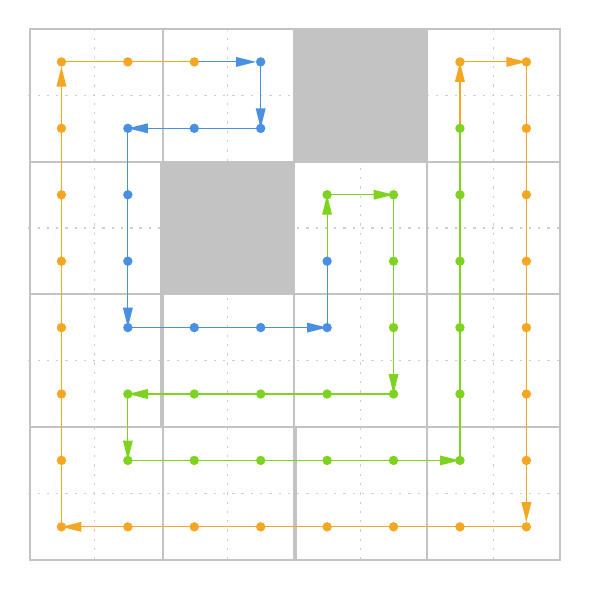
\begin{tikzpicture}[x=0.75pt,y=0.75pt,yscale=-0.8,xscale=0.8]
			%uncomment if require: \path (0,409); %set diagram left start at 0, and has height of 409
			
			%Straight Lines [id:da5351549802319371] 
			\draw [color={rgb, 255:red, 126; green, 211; blue, 33 }  ,draw opacity=1 ]   (351,195) -- (351,157) ;
			\draw [shift={(351,155)}, rotate = 450] [fill={rgb, 255:red, 126; green, 211; blue, 33 }  ,fill opacity=1 ][line width=0.08]  [draw opacity=0] (12,-3) -- (0,0) -- (12,3) -- cycle    ;
			%Straight Lines [id:da21302010090140722] 
			\draw [color={rgb, 255:red, 74; green, 144; blue, 226 }  ,draw opacity=1 ]   (271,75) -- (306.17,75) ;
			\draw [shift={(308.17,75)}, rotate = 180] [fill={rgb, 255:red, 74; green, 144; blue, 226 }  ,fill opacity=1 ][line width=0.08]  [draw opacity=0] (12,-3) -- (0,0) -- (12,3) -- cycle    ;
			%Straight Lines [id:da854517458794269] 
			\draw [color={rgb, 255:red, 195; green, 195; blue, 195 }  ,draw opacity=0.8 ] [dash pattern={on 0.84pt off 2.51pt}]  (211,55) -- (211,375) ;
			%Straight Lines [id:da5657085791005156] 
			\draw [color={rgb, 255:red, 195; green, 195; blue, 195 }  ,draw opacity=0.8 ] [dash pattern={on 0.84pt off 2.51pt}]  (291,55) -- (291,375) ;
			%Straight Lines [id:da2718901706564181] 
			\draw [color={rgb, 255:red, 195; green, 195; blue, 195 }  ,draw opacity=0.8 ] [dash pattern={on 0.84pt off 2.51pt}]  (371,55) -- (371,375) ;
			%Straight Lines [id:da02094912115129599] 
			\draw [color={rgb, 255:red, 195; green, 195; blue, 195 }  ,draw opacity=0.8 ] [dash pattern={on 0.84pt off 2.51pt}]  (451,55) -- (451,375) ;
			%Straight Lines [id:da9533932703135517] 
			\draw [color={rgb, 255:red, 195; green, 195; blue, 195 }  ,draw opacity=0.8 ] [dash pattern={on 0.84pt off 2.51pt}]  (171,95) -- (491,95) ;
			%Straight Lines [id:da9004292598975747] 
			\draw [color={rgb, 255:red, 195; green, 195; blue, 195 }  ,draw opacity=0.8 ] [dash pattern={on 0.84pt off 2.51pt}]  (171,175) -- (491,175) ;
			%Straight Lines [id:da1627688683660009] 
			\draw [color={rgb, 255:red, 195; green, 195; blue, 195 }  ,draw opacity=0.8 ] [dash pattern={on 0.84pt off 2.51pt}]  (171,255) -- (491,255) ;
			%Straight Lines [id:da4991285432755932] 
			\draw [color={rgb, 255:red, 195; green, 195; blue, 195 }  ,draw opacity=0.8 ] [dash pattern={on 0.84pt off 2.51pt}]  (171,335) -- (491,335) ;
			
			%Straight Lines [id:da7491713727663103] 
			\draw [color={rgb, 255:red, 245; green, 166; blue, 35 }  ,draw opacity=1 ]   (431,115) -- (431,77) ;
			\draw [shift={(431,75)}, rotate = 450] [fill={rgb, 255:red, 245; green, 166; blue, 35 }  ,fill opacity=1 ][line width=0.08]  [draw opacity=0] (12,-3) -- (0,0) -- (12,3) -- cycle    ;
			%Shape: Rectangle [id:dp8746081557149701] 
			\draw  [color={rgb, 255:red, 195; green, 195; blue, 195 }  ,draw opacity=1 ][line width=0.75]  (411,55) -- (491,55) -- (491,135) -- (411,135) -- cycle ;
			%Shape: Rectangle [id:dp04998372489748726] 
			\draw  [color={rgb, 255:red, 195; green, 195; blue, 195 }  ,draw opacity=1 ][line width=0.75]  (411,135) -- (491,135) -- (491,215) -- (411,215) -- cycle ;
			%Shape: Rectangle [id:dp716343211155213] 
			\draw  [color={rgb, 255:red, 195; green, 195; blue, 195 }  ,draw opacity=1 ][line width=0.75]  (411,215) -- (491,215) -- (491,295) -- (411,295) -- cycle ;
			%Shape: Rectangle [id:dp9628316526459462] 
			\draw  [color={rgb, 255:red, 195; green, 195; blue, 195 }  ,draw opacity=1 ][line width=0.75]  (411,295) -- (491,295) -- (491,375) -- (411,375) -- cycle ;
			%Shape: Rectangle [id:dp664440026053819] 
			\draw  [color={rgb, 255:red, 195; green, 195; blue, 195 }  ,draw opacity=1 ][line width=0.75]  (331,135) -- (411,135) -- (411,215) -- (331,215) -- cycle ;
			%Shape: Rectangle [id:dp08410695657353351] 
			\draw  [color={rgb, 255:red, 195; green, 195; blue, 195 }  ,draw opacity=1 ][line width=0.75]  (331,215) -- (411,215) -- (411,295) -- (331,295) -- cycle ;
			%Shape: Rectangle [id:dp07090445501331866] 
			\draw  [color={rgb, 255:red, 195; green, 195; blue, 195 }  ,draw opacity=1 ][line width=0.75]  (331,295) -- (411,295) -- (411,375) -- (331,375) -- cycle ;
			%Shape: Rectangle [id:dp8696408090436851] 
			\draw  [color={rgb, 255:red, 195; green, 195; blue, 195 }  ,draw opacity=1 ][line width=0.75]  (252,55) -- (332,55) -- (332,135) -- (252,135) -- cycle ;
			%Shape: Rectangle [id:dp4746238836207364] 
			\draw  [color={rgb, 255:red, 195; green, 195; blue, 195 }  ,draw opacity=1 ][line width=0.75]  (172,55) -- (252,55) -- (252,135) -- (172,135) -- cycle ;
			%Shape: Rectangle [id:dp8657981727821324] 
			\draw  [color={rgb, 255:red, 195; green, 195; blue, 195 }  ,draw opacity=1 ][line width=0.75]  (172,135) -- (252,135) -- (252,215) -- (172,215) -- cycle ;
			%Shape: Rectangle [id:dp20551199499502526] 
			\draw  [color={rgb, 255:red, 195; green, 195; blue, 195 }  ,draw opacity=1 ][line width=0.75]  (172,215) -- (252,215) -- (252,295) -- (172,295) -- cycle ;
			%Shape: Rectangle [id:dp5033014313679982] 
			\draw  [color={rgb, 255:red, 195; green, 195; blue, 195 }  ,draw opacity=1 ][line width=0.75]  (172,295) -- (252,295) -- (252,375) -- (172,375) -- cycle ;
			%Shape: Rectangle [id:dp0691160736423535] 
			\draw  [color={rgb, 255:red, 195; green, 195; blue, 195 }  ,draw opacity=1 ][line width=0.75]  (251,215) -- (331,215) -- (331,295) -- (251,295) -- cycle ;
			%Shape: Rectangle [id:dp9673109533181607] 
			\draw  [color={rgb, 255:red, 195; green, 195; blue, 195 }  ,draw opacity=1 ][line width=0.75]  (252,295) -- (332,295) -- (332,375) -- (252,375) -- cycle ;
			
			%Shape: Rectangle [id:dp24113727014203779] 
			\draw  [color={rgb, 255:red, 195; green, 195; blue, 195 }  ,draw opacity=1 ][fill={rgb, 255:red, 195; green, 195; blue, 195 }  ,fill opacity=1 ][line width=0.75]  (331,55) -- (411,55) -- (411,135) -- (331,135) -- cycle ;
			%Shape: Rectangle [id:dp6453850559631755] 
			\draw  [color={rgb, 255:red, 195; green, 195; blue, 195 }  ,draw opacity=1 ][fill={rgb, 255:red, 195; green, 195; blue, 195 }  ,fill opacity=1 ][line width=0.75]  (251,135) -- (331,135) -- (331,215) -- (251,215) -- cycle ;
			%Shape: Circle [id:dp6801416953242614] 
			\draw  [draw opacity=0][fill={rgb, 255:red, 245; green, 166; blue, 35 }  ,fill opacity=1 ] (468.17,75) .. controls (468.17,73.43) and (469.43,72.17) .. (471,72.17) .. controls (472.57,72.17) and (473.83,73.43) .. (473.83,75) .. controls (473.83,76.57) and (472.57,77.83) .. (471,77.83) .. controls (469.43,77.83) and (468.17,76.57) .. (468.17,75) -- cycle ;
			%Shape: Circle [id:dp4604608393759837] 
			\draw  [draw opacity=0][fill={rgb, 255:red, 245; green, 166; blue, 35 }  ,fill opacity=1 ] (428.17,75) .. controls (428.17,73.43) and (429.43,72.17) .. (431,72.17) .. controls (432.57,72.17) and (433.83,73.43) .. (433.83,75) .. controls (433.83,76.57) and (432.57,77.83) .. (431,77.83) .. controls (429.43,77.83) and (428.17,76.57) .. (428.17,75) -- cycle ;
			%Shape: Circle [id:dp13822592778240006] 
			\draw  [draw opacity=0][fill={rgb, 255:red, 245; green, 166; blue, 35 }  ,fill opacity=1 ] (468.17,115) .. controls (468.17,113.43) and (469.43,112.17) .. (471,112.17) .. controls (472.57,112.17) and (473.83,113.43) .. (473.83,115) .. controls (473.83,116.57) and (472.57,117.83) .. (471,117.83) .. controls (469.43,117.83) and (468.17,116.57) .. (468.17,115) -- cycle ;
			%Shape: Circle [id:dp544207653797784] 
			\draw  [draw opacity=0][fill={rgb, 255:red, 245; green, 166; blue, 35 }  ,fill opacity=1 ] (468.17,155) .. controls (468.17,153.43) and (469.43,152.17) .. (471,152.17) .. controls (472.57,152.17) and (473.83,153.43) .. (473.83,155) .. controls (473.83,156.57) and (472.57,157.83) .. (471,157.83) .. controls (469.43,157.83) and (468.17,156.57) .. (468.17,155) -- cycle ;
			%Shape: Circle [id:dp4171778626191891] 
			\draw  [draw opacity=0][fill={rgb, 255:red, 245; green, 166; blue, 35 }  ,fill opacity=1 ] (468.17,195) .. controls (468.17,193.43) and (469.43,192.17) .. (471,192.17) .. controls (472.57,192.17) and (473.83,193.43) .. (473.83,195) .. controls (473.83,196.57) and (472.57,197.83) .. (471,197.83) .. controls (469.43,197.83) and (468.17,196.57) .. (468.17,195) -- cycle ;
			%Shape: Circle [id:dp7895311637274933] 
			\draw  [draw opacity=0][fill={rgb, 255:red, 245; green, 166; blue, 35 }  ,fill opacity=1 ] (468.17,235) .. controls (468.17,233.43) and (469.43,232.17) .. (471,232.17) .. controls (472.57,232.17) and (473.83,233.43) .. (473.83,235) .. controls (473.83,236.57) and (472.57,237.83) .. (471,237.83) .. controls (469.43,237.83) and (468.17,236.57) .. (468.17,235) -- cycle ;
			%Shape: Circle [id:dp16643331735014688] 
			\draw  [draw opacity=0][fill={rgb, 255:red, 245; green, 166; blue, 35 }  ,fill opacity=1 ] (468.17,275) .. controls (468.17,273.43) and (469.43,272.17) .. (471,272.17) .. controls (472.57,272.17) and (473.83,273.43) .. (473.83,275) .. controls (473.83,276.57) and (472.57,277.83) .. (471,277.83) .. controls (469.43,277.83) and (468.17,276.57) .. (468.17,275) -- cycle ;
			%Shape: Circle [id:dp4612402233444193] 
			\draw  [draw opacity=0][fill={rgb, 255:red, 245; green, 166; blue, 35 }  ,fill opacity=1 ] (468.17,315) .. controls (468.17,313.43) and (469.43,312.17) .. (471,312.17) .. controls (472.57,312.17) and (473.83,313.43) .. (473.83,315) .. controls (473.83,316.57) and (472.57,317.83) .. (471,317.83) .. controls (469.43,317.83) and (468.17,316.57) .. (468.17,315) -- cycle ;
			%Shape: Circle [id:dp10168213951386096] 
			\draw  [draw opacity=0][fill={rgb, 255:red, 245; green, 166; blue, 35 }  ,fill opacity=1 ] (468.17,355) .. controls (468.17,353.43) and (469.43,352.17) .. (471,352.17) .. controls (472.57,352.17) and (473.83,353.43) .. (473.83,355) .. controls (473.83,356.57) and (472.57,357.83) .. (471,357.83) .. controls (469.43,357.83) and (468.17,356.57) .. (468.17,355) -- cycle ;
			%Shape: Circle [id:dp16583621916165892] 
			\draw  [draw opacity=0][fill={rgb, 255:red, 245; green, 166; blue, 35 }  ,fill opacity=1 ] (428.17,355) .. controls (428.17,353.43) and (429.43,352.17) .. (431,352.17) .. controls (432.57,352.17) and (433.83,353.43) .. (433.83,355) .. controls (433.83,356.57) and (432.57,357.83) .. (431,357.83) .. controls (429.43,357.83) and (428.17,356.57) .. (428.17,355) -- cycle ;
			%Shape: Circle [id:dp23056644975317875] 
			\draw  [draw opacity=0][fill={rgb, 255:red, 245; green, 166; blue, 35 }  ,fill opacity=1 ] (388.17,355) .. controls (388.17,353.43) and (389.43,352.17) .. (391,352.17) .. controls (392.57,352.17) and (393.83,353.43) .. (393.83,355) .. controls (393.83,356.57) and (392.57,357.83) .. (391,357.83) .. controls (389.43,357.83) and (388.17,356.57) .. (388.17,355) -- cycle ;
			%Shape: Circle [id:dp8401836553855346] 
			\draw  [draw opacity=0][fill={rgb, 255:red, 245; green, 166; blue, 35 }  ,fill opacity=1 ] (348.17,355) .. controls (348.17,353.43) and (349.43,352.17) .. (351,352.17) .. controls (352.57,352.17) and (353.83,353.43) .. (353.83,355) .. controls (353.83,356.57) and (352.57,357.83) .. (351,357.83) .. controls (349.43,357.83) and (348.17,356.57) .. (348.17,355) -- cycle ;
			%Shape: Circle [id:dp48282190307261685] 
			\draw  [draw opacity=0][fill={rgb, 255:red, 245; green, 166; blue, 35 }  ,fill opacity=1 ] (308.17,355) .. controls (308.17,353.43) and (309.43,352.17) .. (311,352.17) .. controls (312.57,352.17) and (313.83,353.43) .. (313.83,355) .. controls (313.83,356.57) and (312.57,357.83) .. (311,357.83) .. controls (309.43,357.83) and (308.17,356.57) .. (308.17,355) -- cycle ;
			%Shape: Circle [id:dp5761975450405177] 
			\draw  [draw opacity=0][fill={rgb, 255:red, 245; green, 166; blue, 35 }  ,fill opacity=1 ] (268.17,355) .. controls (268.17,353.43) and (269.43,352.17) .. (271,352.17) .. controls (272.57,352.17) and (273.83,353.43) .. (273.83,355) .. controls (273.83,356.57) and (272.57,357.83) .. (271,357.83) .. controls (269.43,357.83) and (268.17,356.57) .. (268.17,355) -- cycle ;
			%Shape: Circle [id:dp06870423995803909] 
			\draw  [draw opacity=0][fill={rgb, 255:red, 245; green, 166; blue, 35 }  ,fill opacity=1 ] (228.17,355) .. controls (228.17,353.43) and (229.43,352.17) .. (231,352.17) .. controls (232.57,352.17) and (233.83,353.43) .. (233.83,355) .. controls (233.83,356.57) and (232.57,357.83) .. (231,357.83) .. controls (229.43,357.83) and (228.17,356.57) .. (228.17,355) -- cycle ;
			%Shape: Circle [id:dp5381906142714585] 
			\draw  [draw opacity=0][fill={rgb, 255:red, 245; green, 166; blue, 35 }  ,fill opacity=1 ] (188.17,355) .. controls (188.17,353.43) and (189.43,352.17) .. (191,352.17) .. controls (192.57,352.17) and (193.83,353.43) .. (193.83,355) .. controls (193.83,356.57) and (192.57,357.83) .. (191,357.83) .. controls (189.43,357.83) and (188.17,356.57) .. (188.17,355) -- cycle ;
			%Shape: Circle [id:dp03637900283495887] 
			\draw  [draw opacity=0][fill={rgb, 255:red, 245; green, 166; blue, 35 }  ,fill opacity=1 ] (188.17,315) .. controls (188.17,313.43) and (189.43,312.17) .. (191,312.17) .. controls (192.57,312.17) and (193.83,313.43) .. (193.83,315) .. controls (193.83,316.57) and (192.57,317.83) .. (191,317.83) .. controls (189.43,317.83) and (188.17,316.57) .. (188.17,315) -- cycle ;
			%Shape: Circle [id:dp5512808090993917] 
			\draw  [draw opacity=0][fill={rgb, 255:red, 245; green, 166; blue, 35 }  ,fill opacity=1 ] (188.17,275) .. controls (188.17,273.43) and (189.43,272.17) .. (191,272.17) .. controls (192.57,272.17) and (193.83,273.43) .. (193.83,275) .. controls (193.83,276.57) and (192.57,277.83) .. (191,277.83) .. controls (189.43,277.83) and (188.17,276.57) .. (188.17,275) -- cycle ;
			%Shape: Circle [id:dp7146308141223112] 
			\draw  [draw opacity=0][fill={rgb, 255:red, 245; green, 166; blue, 35 }  ,fill opacity=1 ] (188.17,235) .. controls (188.17,233.43) and (189.43,232.17) .. (191,232.17) .. controls (192.57,232.17) and (193.83,233.43) .. (193.83,235) .. controls (193.83,236.57) and (192.57,237.83) .. (191,237.83) .. controls (189.43,237.83) and (188.17,236.57) .. (188.17,235) -- cycle ;
			%Shape: Circle [id:dp5335478422961473] 
			\draw  [draw opacity=0][fill={rgb, 255:red, 245; green, 166; blue, 35 }  ,fill opacity=1 ] (188.17,195) .. controls (188.17,193.43) and (189.43,192.17) .. (191,192.17) .. controls (192.57,192.17) and (193.83,193.43) .. (193.83,195) .. controls (193.83,196.57) and (192.57,197.83) .. (191,197.83) .. controls (189.43,197.83) and (188.17,196.57) .. (188.17,195) -- cycle ;
			%Shape: Circle [id:dp8716915789137862] 
			\draw  [draw opacity=0][fill={rgb, 255:red, 245; green, 166; blue, 35 }  ,fill opacity=1 ] (188.17,155) .. controls (188.17,153.43) and (189.43,152.17) .. (191,152.17) .. controls (192.57,152.17) and (193.83,153.43) .. (193.83,155) .. controls (193.83,156.57) and (192.57,157.83) .. (191,157.83) .. controls (189.43,157.83) and (188.17,156.57) .. (188.17,155) -- cycle ;
			%Shape: Circle [id:dp3349585094431857] 
			\draw  [draw opacity=0][fill={rgb, 255:red, 245; green, 166; blue, 35 }  ,fill opacity=1 ] (188.17,115) .. controls (188.17,113.43) and (189.43,112.17) .. (191,112.17) .. controls (192.57,112.17) and (193.83,113.43) .. (193.83,115) .. controls (193.83,116.57) and (192.57,117.83) .. (191,117.83) .. controls (189.43,117.83) and (188.17,116.57) .. (188.17,115) -- cycle ;
			%Shape: Circle [id:dp44273518739120976] 
			\draw  [draw opacity=0][fill={rgb, 255:red, 245; green, 166; blue, 35 }  ,fill opacity=1 ] (188.17,75) .. controls (188.17,73.43) and (189.43,72.17) .. (191,72.17) .. controls (192.57,72.17) and (193.83,73.43) .. (193.83,75) .. controls (193.83,76.57) and (192.57,77.83) .. (191,77.83) .. controls (189.43,77.83) and (188.17,76.57) .. (188.17,75) -- cycle ;
			%Shape: Circle [id:dp8508549485124735] 
			\draw  [draw opacity=0][fill={rgb, 255:red, 245; green, 166; blue, 35 }  ,fill opacity=1 ] (228.17,75) .. controls (228.17,73.43) and (229.43,72.17) .. (231,72.17) .. controls (232.57,72.17) and (233.83,73.43) .. (233.83,75) .. controls (233.83,76.57) and (232.57,77.83) .. (231,77.83) .. controls (229.43,77.83) and (228.17,76.57) .. (228.17,75) -- cycle ;
			%Shape: Circle [id:dp6783308931260619] 
			\draw  [draw opacity=0][fill={rgb, 255:red, 245; green, 166; blue, 35 }  ,fill opacity=1 ] (268.17,75) .. controls (268.17,73.43) and (269.43,72.17) .. (271,72.17) .. controls (272.57,72.17) and (273.83,73.43) .. (273.83,75) .. controls (273.83,76.57) and (272.57,77.83) .. (271,77.83) .. controls (269.43,77.83) and (268.17,76.57) .. (268.17,75) -- cycle ;
			%Straight Lines [id:da5456587577326129] 
			\draw [color={rgb, 255:red, 245; green, 166; blue, 35 }  ,draw opacity=1 ]   (431,75) -- (469,75) ;
			\draw [shift={(471,75)}, rotate = 180] [fill={rgb, 255:red, 245; green, 166; blue, 35 }  ,fill opacity=1 ][line width=0.08]  [draw opacity=0] (12,-3) -- (0,0) -- (12,3) -- cycle    ;
			%Shape: Circle [id:dp4443238058444041] 
			\draw  [draw opacity=0][fill={rgb, 255:red, 74; green, 144; blue, 226 }  ,fill opacity=1 ] (308.17,75) .. controls (308.17,73.43) and (309.43,72.17) .. (311,72.17) .. controls (312.57,72.17) and (313.83,73.43) .. (313.83,75) .. controls (313.83,76.57) and (312.57,77.83) .. (311,77.83) .. controls (309.43,77.83) and (308.17,76.57) .. (308.17,75) -- cycle ;
			%Shape: Circle [id:dp29010302295723345] 
			\draw  [draw opacity=0][fill={rgb, 255:red, 74; green, 144; blue, 226 }  ,fill opacity=1 ] (308.17,115) .. controls (308.17,113.43) and (309.43,112.17) .. (311,112.17) .. controls (312.57,112.17) and (313.83,113.43) .. (313.83,115) .. controls (313.83,116.57) and (312.57,117.83) .. (311,117.83) .. controls (309.43,117.83) and (308.17,116.57) .. (308.17,115) -- cycle ;
			%Shape: Circle [id:dp6216098523896874] 
			\draw  [draw opacity=0][fill={rgb, 255:red, 74; green, 144; blue, 226 }  ,fill opacity=1 ] (268.17,115) .. controls (268.17,113.43) and (269.43,112.17) .. (271,112.17) .. controls (272.57,112.17) and (273.83,113.43) .. (273.83,115) .. controls (273.83,116.57) and (272.57,117.83) .. (271,117.83) .. controls (269.43,117.83) and (268.17,116.57) .. (268.17,115) -- cycle ;
			%Shape: Circle [id:dp06234830362754895] 
			\draw  [draw opacity=0][fill={rgb, 255:red, 74; green, 144; blue, 226 }  ,fill opacity=1 ] (228.17,115) .. controls (228.17,113.43) and (229.43,112.17) .. (231,112.17) .. controls (232.57,112.17) and (233.83,113.43) .. (233.83,115) .. controls (233.83,116.57) and (232.57,117.83) .. (231,117.83) .. controls (229.43,117.83) and (228.17,116.57) .. (228.17,115) -- cycle ;
			%Shape: Circle [id:dp9885173496004662] 
			\draw  [draw opacity=0][fill={rgb, 255:red, 74; green, 144; blue, 226 }  ,fill opacity=1 ] (228.17,155) .. controls (228.17,153.43) and (229.43,152.17) .. (231,152.17) .. controls (232.57,152.17) and (233.83,153.43) .. (233.83,155) .. controls (233.83,156.57) and (232.57,157.83) .. (231,157.83) .. controls (229.43,157.83) and (228.17,156.57) .. (228.17,155) -- cycle ;
			%Shape: Circle [id:dp9444674235776642] 
			\draw  [draw opacity=0][fill={rgb, 255:red, 74; green, 144; blue, 226 }  ,fill opacity=1 ] (228.17,195) .. controls (228.17,193.43) and (229.43,192.17) .. (231,192.17) .. controls (232.57,192.17) and (233.83,193.43) .. (233.83,195) .. controls (233.83,196.57) and (232.57,197.83) .. (231,197.83) .. controls (229.43,197.83) and (228.17,196.57) .. (228.17,195) -- cycle ;
			%Shape: Circle [id:dp7868027408873275] 
			\draw  [draw opacity=0][fill={rgb, 255:red, 74; green, 144; blue, 226 }  ,fill opacity=1 ] (228.17,235) .. controls (228.17,233.43) and (229.43,232.17) .. (231,232.17) .. controls (232.57,232.17) and (233.83,233.43) .. (233.83,235) .. controls (233.83,236.57) and (232.57,237.83) .. (231,237.83) .. controls (229.43,237.83) and (228.17,236.57) .. (228.17,235) -- cycle ;
			%Shape: Circle [id:dp35955963628126275] 
			\draw  [draw opacity=0][fill={rgb, 255:red, 74; green, 144; blue, 226 }  ,fill opacity=1 ] (268.17,235) .. controls (268.17,233.43) and (269.43,232.17) .. (271,232.17) .. controls (272.57,232.17) and (273.83,233.43) .. (273.83,235) .. controls (273.83,236.57) and (272.57,237.83) .. (271,237.83) .. controls (269.43,237.83) and (268.17,236.57) .. (268.17,235) -- cycle ;
			%Shape: Circle [id:dp5516376120857398] 
			\draw  [draw opacity=0][fill={rgb, 255:red, 74; green, 144; blue, 226 }  ,fill opacity=1 ] (308.17,235) .. controls (308.17,233.43) and (309.43,232.17) .. (311,232.17) .. controls (312.57,232.17) and (313.83,233.43) .. (313.83,235) .. controls (313.83,236.57) and (312.57,237.83) .. (311,237.83) .. controls (309.43,237.83) and (308.17,236.57) .. (308.17,235) -- cycle ;
			%Shape: Circle [id:dp5893700740487555] 
			\draw  [draw opacity=0][fill={rgb, 255:red, 74; green, 144; blue, 226 }  ,fill opacity=1 ] (348.17,235) .. controls (348.17,233.43) and (349.43,232.17) .. (351,232.17) .. controls (352.57,232.17) and (353.83,233.43) .. (353.83,235) .. controls (353.83,236.57) and (352.57,237.83) .. (351,237.83) .. controls (349.43,237.83) and (348.17,236.57) .. (348.17,235) -- cycle ;
			%Shape: Circle [id:dp1286587461477784] 
			\draw  [draw opacity=0][fill={rgb, 255:red, 74; green, 144; blue, 226 }  ,fill opacity=1 ] (348.17,195) .. controls (348.17,193.43) and (349.43,192.17) .. (351,192.17) .. controls (352.57,192.17) and (353.83,193.43) .. (353.83,195) .. controls (353.83,196.57) and (352.57,197.83) .. (351,197.83) .. controls (349.43,197.83) and (348.17,196.57) .. (348.17,195) -- cycle ;
			%Shape: Circle [id:dp26088941378322006] 
			\draw  [draw opacity=0][fill={rgb, 255:red, 126; green, 211; blue, 33 }  ,fill opacity=1 ] (348.17,155) .. controls (348.17,153.43) and (349.43,152.17) .. (351,152.17) .. controls (352.57,152.17) and (353.83,153.43) .. (353.83,155) .. controls (353.83,156.57) and (352.57,157.83) .. (351,157.83) .. controls (349.43,157.83) and (348.17,156.57) .. (348.17,155) -- cycle ;
			%Shape: Circle [id:dp9676514649936712] 
			\draw  [draw opacity=0][fill={rgb, 255:red, 126; green, 211; blue, 33 }  ,fill opacity=1 ] (388.17,155) .. controls (388.17,153.43) and (389.43,152.17) .. (391,152.17) .. controls (392.57,152.17) and (393.83,153.43) .. (393.83,155) .. controls (393.83,156.57) and (392.57,157.83) .. (391,157.83) .. controls (389.43,157.83) and (388.17,156.57) .. (388.17,155) -- cycle ;
			%Shape: Circle [id:dp19213789582339302] 
			\draw  [draw opacity=0][fill={rgb, 255:red, 126; green, 211; blue, 33 }  ,fill opacity=1 ] (388.17,195) .. controls (388.17,193.43) and (389.43,192.17) .. (391,192.17) .. controls (392.57,192.17) and (393.83,193.43) .. (393.83,195) .. controls (393.83,196.57) and (392.57,197.83) .. (391,197.83) .. controls (389.43,197.83) and (388.17,196.57) .. (388.17,195) -- cycle ;
			%Shape: Circle [id:dp31757377829209155] 
			\draw  [draw opacity=0][fill={rgb, 255:red, 126; green, 211; blue, 33 }  ,fill opacity=1 ] (388.17,235) .. controls (388.17,233.43) and (389.43,232.17) .. (391,232.17) .. controls (392.57,232.17) and (393.83,233.43) .. (393.83,235) .. controls (393.83,236.57) and (392.57,237.83) .. (391,237.83) .. controls (389.43,237.83) and (388.17,236.57) .. (388.17,235) -- cycle ;
			%Shape: Circle [id:dp11411146161431085] 
			\draw  [draw opacity=0][fill={rgb, 255:red, 126; green, 211; blue, 33 }  ,fill opacity=1 ] (388.17,275) .. controls (388.17,273.43) and (389.43,272.17) .. (391,272.17) .. controls (392.57,272.17) and (393.83,273.43) .. (393.83,275) .. controls (393.83,276.57) and (392.57,277.83) .. (391,277.83) .. controls (389.43,277.83) and (388.17,276.57) .. (388.17,275) -- cycle ;
			%Shape: Circle [id:dp6075376860133745] 
			\draw  [draw opacity=0][fill={rgb, 255:red, 126; green, 211; blue, 33 }  ,fill opacity=1 ] (348.17,275) .. controls (348.17,273.43) and (349.43,272.17) .. (351,272.17) .. controls (352.57,272.17) and (353.83,273.43) .. (353.83,275) .. controls (353.83,276.57) and (352.57,277.83) .. (351,277.83) .. controls (349.43,277.83) and (348.17,276.57) .. (348.17,275) -- cycle ;
			%Shape: Circle [id:dp33787943985666535] 
			\draw  [draw opacity=0][fill={rgb, 255:red, 126; green, 211; blue, 33 }  ,fill opacity=1 ] (308.17,275) .. controls (308.17,273.43) and (309.43,272.17) .. (311,272.17) .. controls (312.57,272.17) and (313.83,273.43) .. (313.83,275) .. controls (313.83,276.57) and (312.57,277.83) .. (311,277.83) .. controls (309.43,277.83) and (308.17,276.57) .. (308.17,275) -- cycle ;
			%Shape: Circle [id:dp6967659869352532] 
			\draw  [draw opacity=0][fill={rgb, 255:red, 126; green, 211; blue, 33 }  ,fill opacity=1 ] (268.17,275) .. controls (268.17,273.43) and (269.43,272.17) .. (271,272.17) .. controls (272.57,272.17) and (273.83,273.43) .. (273.83,275) .. controls (273.83,276.57) and (272.57,277.83) .. (271,277.83) .. controls (269.43,277.83) and (268.17,276.57) .. (268.17,275) -- cycle ;
			%Shape: Circle [id:dp7916368779271419] 
			\draw  [draw opacity=0][fill={rgb, 255:red, 126; green, 211; blue, 33 }  ,fill opacity=1 ] (228.17,275) .. controls (228.17,273.43) and (229.43,272.17) .. (231,272.17) .. controls (232.57,272.17) and (233.83,273.43) .. (233.83,275) .. controls (233.83,276.57) and (232.57,277.83) .. (231,277.83) .. controls (229.43,277.83) and (228.17,276.57) .. (228.17,275) -- cycle ;
			%Shape: Circle [id:dp9131057577477717] 
			\draw  [draw opacity=0][fill={rgb, 255:red, 126; green, 211; blue, 33 }  ,fill opacity=1 ] (228.17,315) .. controls (228.17,313.43) and (229.43,312.17) .. (231,312.17) .. controls (232.57,312.17) and (233.83,313.43) .. (233.83,315) .. controls (233.83,316.57) and (232.57,317.83) .. (231,317.83) .. controls (229.43,317.83) and (228.17,316.57) .. (228.17,315) -- cycle ;
			%Shape: Circle [id:dp060540910098607625] 
			\draw  [draw opacity=0][fill={rgb, 255:red, 126; green, 211; blue, 33 }  ,fill opacity=1 ] (268.17,315) .. controls (268.17,313.43) and (269.43,312.17) .. (271,312.17) .. controls (272.57,312.17) and (273.83,313.43) .. (273.83,315) .. controls (273.83,316.57) and (272.57,317.83) .. (271,317.83) .. controls (269.43,317.83) and (268.17,316.57) .. (268.17,315) -- cycle ;
			%Shape: Circle [id:dp4358067111786901] 
			\draw  [draw opacity=0][fill={rgb, 255:red, 126; green, 211; blue, 33 }  ,fill opacity=1 ] (308.17,315) .. controls (308.17,313.43) and (309.43,312.17) .. (311,312.17) .. controls (312.57,312.17) and (313.83,313.43) .. (313.83,315) .. controls (313.83,316.57) and (312.57,317.83) .. (311,317.83) .. controls (309.43,317.83) and (308.17,316.57) .. (308.17,315) -- cycle ;
			%Shape: Circle [id:dp6562545880538291] 
			\draw  [draw opacity=0][fill={rgb, 255:red, 126; green, 211; blue, 33 }  ,fill opacity=1 ] (348.17,315) .. controls (348.17,313.43) and (349.43,312.17) .. (351,312.17) .. controls (352.57,312.17) and (353.83,313.43) .. (353.83,315) .. controls (353.83,316.57) and (352.57,317.83) .. (351,317.83) .. controls (349.43,317.83) and (348.17,316.57) .. (348.17,315) -- cycle ;
			%Shape: Circle [id:dp18058415370378111] 
			\draw  [draw opacity=0][fill={rgb, 255:red, 126; green, 211; blue, 33 }  ,fill opacity=1 ] (388.17,315) .. controls (388.17,313.43) and (389.43,312.17) .. (391,312.17) .. controls (392.57,312.17) and (393.83,313.43) .. (393.83,315) .. controls (393.83,316.57) and (392.57,317.83) .. (391,317.83) .. controls (389.43,317.83) and (388.17,316.57) .. (388.17,315) -- cycle ;
			%Shape: Circle [id:dp10115316904907612] 
			\draw  [draw opacity=0][fill={rgb, 255:red, 126; green, 211; blue, 33 }  ,fill opacity=1 ] (428.17,315) .. controls (428.17,313.43) and (429.43,312.17) .. (431,312.17) .. controls (432.57,312.17) and (433.83,313.43) .. (433.83,315) .. controls (433.83,316.57) and (432.57,317.83) .. (431,317.83) .. controls (429.43,317.83) and (428.17,316.57) .. (428.17,315) -- cycle ;
			%Shape: Circle [id:dp835742083306757] 
			\draw  [draw opacity=0][fill={rgb, 255:red, 126; green, 211; blue, 33 }  ,fill opacity=1 ] (428.17,275) .. controls (428.17,273.43) and (429.43,272.17) .. (431,272.17) .. controls (432.57,272.17) and (433.83,273.43) .. (433.83,275) .. controls (433.83,276.57) and (432.57,277.83) .. (431,277.83) .. controls (429.43,277.83) and (428.17,276.57) .. (428.17,275) -- cycle ;
			%Shape: Circle [id:dp780791295796917] 
			\draw  [draw opacity=0][fill={rgb, 255:red, 126; green, 211; blue, 33 }  ,fill opacity=1 ] (428.17,235) .. controls (428.17,233.43) and (429.43,232.17) .. (431,232.17) .. controls (432.57,232.17) and (433.83,233.43) .. (433.83,235) .. controls (433.83,236.57) and (432.57,237.83) .. (431,237.83) .. controls (429.43,237.83) and (428.17,236.57) .. (428.17,235) -- cycle ;
			%Shape: Circle [id:dp742197015069753] 
			\draw  [draw opacity=0][fill={rgb, 255:red, 126; green, 211; blue, 33 }  ,fill opacity=1 ] (428.17,195) .. controls (428.17,193.43) and (429.43,192.17) .. (431,192.17) .. controls (432.57,192.17) and (433.83,193.43) .. (433.83,195) .. controls (433.83,196.57) and (432.57,197.83) .. (431,197.83) .. controls (429.43,197.83) and (428.17,196.57) .. (428.17,195) -- cycle ;
			%Shape: Circle [id:dp058172723888363365] 
			\draw  [draw opacity=0][fill={rgb, 255:red, 126; green, 211; blue, 33 }  ,fill opacity=1 ] (428.17,155) .. controls (428.17,153.43) and (429.43,152.17) .. (431,152.17) .. controls (432.57,152.17) and (433.83,153.43) .. (433.83,155) .. controls (433.83,156.57) and (432.57,157.83) .. (431,157.83) .. controls (429.43,157.83) and (428.17,156.57) .. (428.17,155) -- cycle ;
			%Shape: Circle [id:dp40603445670354055] 
			\draw  [draw opacity=0][fill={rgb, 255:red, 126; green, 211; blue, 33 }  ,fill opacity=1 ] (428.17,115) .. controls (428.17,113.43) and (429.43,112.17) .. (431,112.17) .. controls (432.57,112.17) and (433.83,113.43) .. (433.83,115) .. controls (433.83,116.57) and (432.57,117.83) .. (431,117.83) .. controls (429.43,117.83) and (428.17,116.57) .. (428.17,115) -- cycle ;
			%Straight Lines [id:da16789636771970073] 
			\draw [color={rgb, 255:red, 245; green, 166; blue, 35 }  ,draw opacity=1 ]   (471,75) -- (471,350.17) ;
			\draw [shift={(471,352.17)}, rotate = 270] [fill={rgb, 255:red, 245; green, 166; blue, 35 }  ,fill opacity=1 ][line width=0.08]  [draw opacity=0] (12,-3) -- (0,0) -- (12,3) -- cycle    ;
			%Straight Lines [id:da3449631876846895] 
			\draw [color={rgb, 255:red, 245; green, 166; blue, 35 }  ,draw opacity=1 ]   (471,355) -- (193,355) ;
			\draw [shift={(191,355)}, rotate = 360] [fill={rgb, 255:red, 245; green, 166; blue, 35 }  ,fill opacity=1 ][line width=0.08]  [draw opacity=0] (12,-3) -- (0,0) -- (12,3) -- cycle    ;
			%Straight Lines [id:da10161365475922346] 
			\draw [color={rgb, 255:red, 245; green, 166; blue, 35 }  ,draw opacity=1 ]   (191,355) -- (191,79.83) ;
			\draw [shift={(191,77.83)}, rotate = 450] [fill={rgb, 255:red, 245; green, 166; blue, 35 }  ,fill opacity=1 ][line width=0.08]  [draw opacity=0] (12,-3) -- (0,0) -- (12,3) -- cycle    ;
			%Straight Lines [id:da8632021686141709] 
			\draw [color={rgb, 255:red, 245; green, 166; blue, 35 }  ,draw opacity=1 ]   (191,75) -- (271,75) ;
			%Straight Lines [id:da7671632448461922] 
			\draw [color={rgb, 255:red, 74; green, 144; blue, 226 }  ,draw opacity=1 ]   (311,75) -- (311,113) ;
			\draw [shift={(311,115)}, rotate = 270] [fill={rgb, 255:red, 74; green, 144; blue, 226 }  ,fill opacity=1 ][line width=0.08]  [draw opacity=0] (12,-3) -- (0,0) -- (12,3) -- cycle    ;
			%Straight Lines [id:da672307594730295] 
			\draw [color={rgb, 255:red, 74; green, 144; blue, 226 }  ,draw opacity=1 ]   (311,115) -- (233,115) ;
			\draw [shift={(231,115)}, rotate = 360] [fill={rgb, 255:red, 74; green, 144; blue, 226 }  ,fill opacity=1 ][line width=0.08]  [draw opacity=0] (12,-3) -- (0,0) -- (12,3) -- cycle    ;
			%Straight Lines [id:da4077834871044419] 
			\draw [color={rgb, 255:red, 74; green, 144; blue, 226 }  ,draw opacity=1 ]   (231,115) -- (231,233) ;
			\draw [shift={(231,235)}, rotate = 270] [fill={rgb, 255:red, 74; green, 144; blue, 226 }  ,fill opacity=1 ][line width=0.08]  [draw opacity=0] (12,-3) -- (0,0) -- (12,3) -- cycle    ;
			%Straight Lines [id:da9346944539277193] 
			\draw [color={rgb, 255:red, 74; green, 144; blue, 226 }  ,draw opacity=1 ]   (231,235) -- (349,235) ;
			\draw [shift={(351,235)}, rotate = 180] [fill={rgb, 255:red, 74; green, 144; blue, 226 }  ,fill opacity=1 ][line width=0.08]  [draw opacity=0] (12,-3) -- (0,0) -- (12,3) -- cycle    ;
			%Straight Lines [id:da6701207435426635] 
			\draw [color={rgb, 255:red, 74; green, 144; blue, 226 }  ,draw opacity=1 ]   (351,235) -- (351,195) ;
			%Straight Lines [id:da5501151214452311] 
			\draw [color={rgb, 255:red, 126; green, 211; blue, 33 }  ,draw opacity=1 ]   (351,155) -- (389,155) ;
			\draw [shift={(391,155)}, rotate = 180] [fill={rgb, 255:red, 126; green, 211; blue, 33 }  ,fill opacity=1 ][line width=0.08]  [draw opacity=0] (12,-3) -- (0,0) -- (12,3) -- cycle    ;
			%Straight Lines [id:da4311911132527191] 
			\draw [color={rgb, 255:red, 126; green, 211; blue, 33 }  ,draw opacity=1 ]   (391,155) -- (391,194) -- (391,273) ;
			\draw [shift={(391,275)}, rotate = 270] [fill={rgb, 255:red, 126; green, 211; blue, 33 }  ,fill opacity=1 ][line width=0.08]  [draw opacity=0] (12,-3) -- (0,0) -- (12,3) -- cycle    ;
			%Straight Lines [id:da5705388383279479] 
			\draw [color={rgb, 255:red, 126; green, 211; blue, 33 }  ,draw opacity=1 ]   (391,275) -- (233,275) ;
			\draw [shift={(231,275)}, rotate = 360] [fill={rgb, 255:red, 126; green, 211; blue, 33 }  ,fill opacity=1 ][line width=0.08]  [draw opacity=0] (12,-3) -- (0,0) -- (12,3) -- cycle    ;
			%Straight Lines [id:da21297417889995085] 
			\draw [color={rgb, 255:red, 126; green, 211; blue, 33 }  ,draw opacity=1 ]   (231,275) -- (231,313) ;
			\draw [shift={(231,315)}, rotate = 270] [fill={rgb, 255:red, 126; green, 211; blue, 33 }  ,fill opacity=1 ][line width=0.08]  [draw opacity=0] (12,-3) -- (0,0) -- (12,3) -- cycle    ;
			%Straight Lines [id:da22819451965736026] 
			\draw [color={rgb, 255:red, 126; green, 211; blue, 33 }  ,draw opacity=1 ]   (231,315) -- (429,315) ;
			\draw [shift={(431,315)}, rotate = 180] [fill={rgb, 255:red, 126; green, 211; blue, 33 }  ,fill opacity=1 ][line width=0.08]  [draw opacity=0] (12,-3) -- (0,0) -- (12,3) -- cycle    ;
			%Straight Lines [id:da7504973565926707] 
			\draw [color={rgb, 255:red, 126; green, 211; blue, 33 }  ,draw opacity=1 ]   (431,315) -- (431,115) ;
			
			
			
			
		\end{tikzpicture}
		\caption{Path generated by generating way-points from arrows}
		\label{fig:wpnts01}
	\end{subfigure}
	\hfill
	\begin{subfigure}{0.45\textwidth}
		\centering
		\tikzset{every picture/.style={line width=0.75pt}} %set default line width to 0.75pt        
		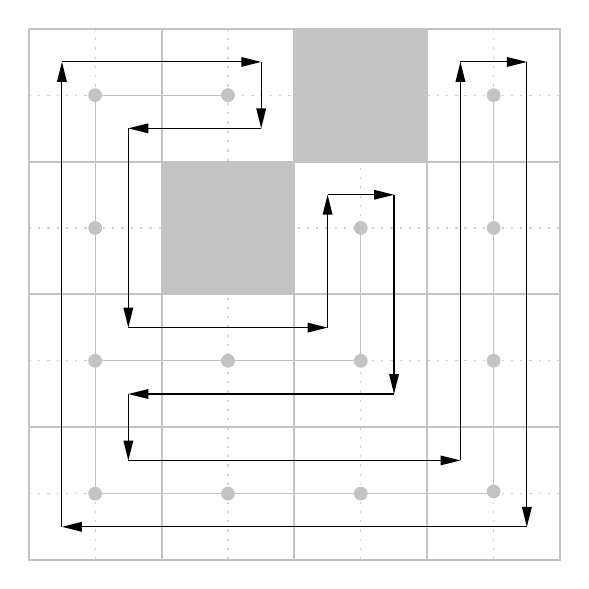
\begin{tikzpicture}[x=0.75pt,y=0.75pt,yscale=-0.8,xscale=0.8]
			%uncomment if require: \path (0,401); %set diagram left start at 0, and has height of 401
			
			%Straight Lines [id:da6525656097654802] 
			\draw [color={rgb, 255:red, 195; green, 195; blue, 195 }  ,draw opacity=0.8 ] [dash pattern={on 0.84pt off 2.51pt}]  (209,36) -- (209,356) ;
			%Straight Lines [id:da9449615822379405] 
			\draw [color={rgb, 255:red, 195; green, 195; blue, 195 }  ,draw opacity=0.8 ] [dash pattern={on 0.84pt off 2.51pt}]  (289,36) -- (289,356) ;
			%Straight Lines [id:da49922694692753367] 
			\draw [color={rgb, 255:red, 195; green, 195; blue, 195 }  ,draw opacity=0.8 ] [dash pattern={on 0.84pt off 2.51pt}]  (369,36) -- (369,356) ;
			%Straight Lines [id:da42403625075839124] 
			\draw [color={rgb, 255:red, 195; green, 195; blue, 195 }  ,draw opacity=0.8 ] [dash pattern={on 0.84pt off 2.51pt}]  (449,36) -- (449,356) ;
			%Straight Lines [id:da41382258883228107] 
			\draw [color={rgb, 255:red, 195; green, 195; blue, 195 }  ,draw opacity=0.8 ] [dash pattern={on 0.84pt off 2.51pt}]  (169,76) -- (489,76) ;
			%Straight Lines [id:da37487046166351323] 
			\draw [color={rgb, 255:red, 195; green, 195; blue, 195 }  ,draw opacity=0.8 ] [dash pattern={on 0.84pt off 2.51pt}]  (169,156) -- (489,156) ;
			%Straight Lines [id:da7805503540839331] 
			\draw [color={rgb, 255:red, 195; green, 195; blue, 195 }  ,draw opacity=0.8 ] [dash pattern={on 0.84pt off 2.51pt}]  (169,236) -- (489,236) ;
			%Straight Lines [id:da0007847063653105835] 
			\draw [color={rgb, 255:red, 195; green, 195; blue, 195 }  ,draw opacity=0.8 ] [dash pattern={on 0.84pt off 2.51pt}]  (169,316) -- (489,316) ;
			
			%Shape: Rectangle [id:dp9282250935920651] 
			\draw  [color={rgb, 255:red, 195; green, 195; blue, 195 }  ,draw opacity=1 ][line width=0.75]  (409,36) -- (489,36) -- (489,116) -- (409,116) -- cycle ;
			%Shape: Rectangle [id:dp40889920048446493] 
			\draw  [color={rgb, 255:red, 195; green, 195; blue, 195 }  ,draw opacity=1 ][line width=0.75]  (409,116) -- (489,116) -- (489,196) -- (409,196) -- cycle ;
			%Shape: Rectangle [id:dp08210856469103622] 
			\draw  [color={rgb, 255:red, 195; green, 195; blue, 195 }  ,draw opacity=1 ][line width=0.75]  (409,196) -- (489,196) -- (489,276) -- (409,276) -- cycle ;
			%Shape: Rectangle [id:dp11132018353927009] 
			\draw  [color={rgb, 255:red, 195; green, 195; blue, 195 }  ,draw opacity=1 ][line width=0.75]  (409,276) -- (489,276) -- (489,356) -- (409,356) -- cycle ;
			%Shape: Rectangle [id:dp056079390985070976] 
			\draw  [color={rgb, 255:red, 195; green, 195; blue, 195 }  ,draw opacity=1 ][line width=0.75]  (329,116) -- (409,116) -- (409,196) -- (329,196) -- cycle ;
			%Shape: Rectangle [id:dp8717884780085985] 
			\draw  [color={rgb, 255:red, 195; green, 195; blue, 195 }  ,draw opacity=1 ][line width=0.75]  (329,196) -- (409,196) -- (409,276) -- (329,276) -- cycle ;
			%Shape: Rectangle [id:dp6966702207831605] 
			\draw  [color={rgb, 255:red, 195; green, 195; blue, 195 }  ,draw opacity=1 ][line width=0.75]  (329,276) -- (409,276) -- (409,356) -- (329,356) -- cycle ;
			%Shape: Rectangle [id:dp6557240237758346] 
			\draw  [color={rgb, 255:red, 195; green, 195; blue, 195 }  ,draw opacity=1 ][line width=0.75]  (249,36) -- (329,36) -- (329,116) -- (249,116) -- cycle ;
			%Shape: Rectangle [id:dp46922355033620544] 
			\draw  [color={rgb, 255:red, 195; green, 195; blue, 195 }  ,draw opacity=1 ][line width=0.75]  (169,36) -- (249,36) -- (249,116) -- (169,116) -- cycle ;
			%Shape: Rectangle [id:dp7130641235448705] 
			\draw  [color={rgb, 255:red, 195; green, 195; blue, 195 }  ,draw opacity=1 ][line width=0.75]  (169,116) -- (249,116) -- (249,196) -- (169,196) -- cycle ;
			%Shape: Rectangle [id:dp8416366697669087] 
			\draw  [color={rgb, 255:red, 195; green, 195; blue, 195 }  ,draw opacity=1 ][line width=0.75]  (169,196) -- (249,196) -- (249,276) -- (169,276) -- cycle ;
			%Shape: Rectangle [id:dp5912644819544948] 
			\draw  [color={rgb, 255:red, 195; green, 195; blue, 195 }  ,draw opacity=1 ][line width=0.75]  (169,276) -- (249,276) -- (249,356) -- (169,356) -- cycle ;
			%Shape: Rectangle [id:dp6447358006368811] 
			\draw  [color={rgb, 255:red, 195; green, 195; blue, 195 }  ,draw opacity=1 ][line width=0.75]  (249,196) -- (329,196) -- (329,276) -- (249,276) -- cycle ;
			%Shape: Rectangle [id:dp8887506508423009] 
			\draw  [color={rgb, 255:red, 195; green, 195; blue, 195 }  ,draw opacity=1 ][line width=0.75]  (249,276) -- (329,276) -- (329,356) -- (249,356) -- cycle ;
			
			%Straight Lines [id:da1738948188181435] 
			\draw [color={rgb, 255:red, 195; green, 195; blue, 195 }  ,draw opacity=1 ]   (209,76) -- (265,76) -- (289,76) ;
			%Straight Lines [id:da7049505215325911] 
			\draw [color={rgb, 255:red, 195; green, 195; blue, 195 }  ,draw opacity=1 ]   (209,76) -- (209,316) ;
			%Straight Lines [id:da9869392385512394] 
			\draw [color={rgb, 255:red, 195; green, 195; blue, 195 }  ,draw opacity=1 ]   (209,316) -- (449,316) ;
			%Straight Lines [id:da1614981151805881] 
			\draw [color={rgb, 255:red, 195; green, 195; blue, 195 }  ,draw opacity=1 ]   (449,77) -- (449,317) ;
			%Straight Lines [id:da45917613825264225] 
			\draw [color={rgb, 255:red, 195; green, 195; blue, 195 }  ,draw opacity=1 ]   (369,237) -- (369,157) ;
			%Straight Lines [id:da6889780670091039] 
			\draw [color={rgb, 255:red, 195; green, 195; blue, 195 }  ,draw opacity=1 ]   (209,236) -- (369,236) ;
			%Straight Lines [id:da12273195124066882] 
			\draw [color={rgb, 255:red, 0; green, 0; blue, 0 }  ,draw opacity=1 ][fill={rgb, 255:red, 0; green, 0; blue, 0 }  ,fill opacity=1 ]   (349,216) -- (349,138) ;
			\draw [shift={(349,136)}, rotate = 450] [fill={rgb, 255:red, 0; green, 0; blue, 0 }  ,fill opacity=1 ][line width=0.08]  [draw opacity=0] (12,-3) -- (0,0) -- (12,3) -- cycle    ;
			%Straight Lines [id:da3917937162075191] 
			\draw [color={rgb, 255:red, 0; green, 0; blue, 0 }  ,draw opacity=1 ][fill={rgb, 255:red, 0; green, 0; blue, 0 }  ,fill opacity=1 ]   (229,216) -- (347,216) ;
			\draw [shift={(349,216)}, rotate = 180] [fill={rgb, 255:red, 0; green, 0; blue, 0 }  ,fill opacity=1 ][line width=0.08]  [draw opacity=0] (12,-3) -- (0,0) -- (12,3) -- cycle    ;
			%Straight Lines [id:da4803441771366592] 
			\draw [color={rgb, 255:red, 0; green, 0; blue, 0 }  ,draw opacity=1 ][fill={rgb, 255:red, 0; green, 0; blue, 0 }  ,fill opacity=1 ]   (229,96) -- (229,214) ;
			\draw [shift={(229,216)}, rotate = 270] [fill={rgb, 255:red, 0; green, 0; blue, 0 }  ,fill opacity=1 ][line width=0.08]  [draw opacity=0] (12,-3) -- (0,0) -- (12,3) -- cycle    ;
			%Straight Lines [id:da7402482792888903] 
			\draw [color={rgb, 255:red, 0; green, 0; blue, 0 }  ,draw opacity=1 ][fill={rgb, 255:red, 0; green, 0; blue, 0 }  ,fill opacity=1 ]   (309,96) -- (231,96) ;
			\draw [shift={(229,96)}, rotate = 360] [fill={rgb, 255:red, 0; green, 0; blue, 0 }  ,fill opacity=1 ][line width=0.08]  [draw opacity=0] (12,-3) -- (0,0) -- (12,3) -- cycle    ;
			%Straight Lines [id:da8948623102095223] 
			\draw [color={rgb, 255:red, 0; green, 0; blue, 0 }  ,draw opacity=1 ][fill={rgb, 255:red, 0; green, 0; blue, 0 }  ,fill opacity=1 ]   (309,56) -- (309,94) ;
			\draw [shift={(309,96)}, rotate = 270] [fill={rgb, 255:red, 0; green, 0; blue, 0 }  ,fill opacity=1 ][line width=0.08]  [draw opacity=0] (12,-3) -- (0,0) -- (12,3) -- cycle    ;
			%Straight Lines [id:da25998808169222265] 
			\draw [color={rgb, 255:red, 0; green, 0; blue, 0 }  ,draw opacity=1 ][fill={rgb, 255:red, 0; green, 0; blue, 0 }  ,fill opacity=1 ]   (189,56) -- (307,56) ;
			\draw [shift={(309,56)}, rotate = 180] [fill={rgb, 255:red, 0; green, 0; blue, 0 }  ,fill opacity=1 ][line width=0.08]  [draw opacity=0] (12,-3) -- (0,0) -- (12,3) -- cycle    ;
			%Straight Lines [id:da40263375664736256] 
			\draw [color={rgb, 255:red, 0; green, 0; blue, 0 }  ,draw opacity=1 ][fill={rgb, 255:red, 0; green, 0; blue, 0 }  ,fill opacity=1 ]   (189,336) -- (189,58) ;
			\draw [shift={(189,56)}, rotate = 450] [fill={rgb, 255:red, 0; green, 0; blue, 0 }  ,fill opacity=1 ][line width=0.08]  [draw opacity=0] (12,-3) -- (0,0) -- (12,3) -- cycle    ;
			%Straight Lines [id:da48570875534448854] 
			\draw [color={rgb, 255:red, 0; green, 0; blue, 0 }  ,draw opacity=1 ][fill={rgb, 255:red, 0; green, 0; blue, 0 }  ,fill opacity=1 ]   (469,336) -- (191,336) ;
			\draw [shift={(189,336)}, rotate = 360] [fill={rgb, 255:red, 0; green, 0; blue, 0 }  ,fill opacity=1 ][line width=0.08]  [draw opacity=0] (12,-3) -- (0,0) -- (12,3) -- cycle    ;
			%Straight Lines [id:da8647185294436568] 
			\draw [color={rgb, 255:red, 0; green, 0; blue, 0 }  ,draw opacity=1 ][fill={rgb, 255:red, 0; green, 0; blue, 0 }  ,fill opacity=1 ]   (469,56) -- (469,334) ;
			\draw [shift={(469,336)}, rotate = 270] [fill={rgb, 255:red, 0; green, 0; blue, 0 }  ,fill opacity=1 ][line width=0.08]  [draw opacity=0] (12,-3) -- (0,0) -- (12,3) -- cycle    ;
			%Straight Lines [id:da5962728530510046] 
			\draw [color={rgb, 255:red, 0; green, 0; blue, 0 }  ,draw opacity=1 ][fill={rgb, 255:red, 0; green, 0; blue, 0 }  ,fill opacity=1 ]   (429,296) -- (429,58) ;
			\draw [shift={(429,56)}, rotate = 450] [fill={rgb, 255:red, 0; green, 0; blue, 0 }  ,fill opacity=1 ][line width=0.08]  [draw opacity=0] (12,-3) -- (0,0) -- (12,3) -- cycle    ;
			%Straight Lines [id:da3206966034529801] 
			\draw [color={rgb, 255:red, 0; green, 0; blue, 0 }  ,draw opacity=1 ][fill={rgb, 255:red, 0; green, 0; blue, 0 }  ,fill opacity=1 ]   (229,296) -- (427,296) ;
			\draw [shift={(429,296)}, rotate = 180] [fill={rgb, 255:red, 0; green, 0; blue, 0 }  ,fill opacity=1 ][line width=0.08]  [draw opacity=0] (12,-3) -- (0,0) -- (12,3) -- cycle    ;
			%Shape: Rectangle [id:dp2343107393386883] 
			\draw  [color={rgb, 255:red, 195; green, 195; blue, 195 }  ,draw opacity=1 ][fill={rgb, 255:red, 195; green, 195; blue, 195 }  ,fill opacity=1 ][line width=0.75]  (329,36) -- (409,36) -- (409,116) -- (329,116) -- cycle ;
			%Shape: Rectangle [id:dp7923981711361026] 
			\draw  [color={rgb, 255:red, 195; green, 195; blue, 195 }  ,draw opacity=1 ][fill={rgb, 255:red, 195; green, 195; blue, 195 }  ,fill opacity=1 ][line width=0.75]  (249,116) -- (329,116) -- (329,196) -- (249,196) -- cycle ;
			%Straight Lines [id:da8657248227410601] 
			\draw [color={rgb, 255:red, 0; green, 0; blue, 0 }  ,draw opacity=1 ][fill={rgb, 255:red, 0; green, 0; blue, 0 }  ,fill opacity=1 ]   (429,56) -- (467,56) ;
			\draw [shift={(469,56)}, rotate = 180] [fill={rgb, 255:red, 0; green, 0; blue, 0 }  ,fill opacity=1 ][line width=0.08]  [draw opacity=0] (12,-3) -- (0,0) -- (12,3) -- cycle    ;
			%Straight Lines [id:da6481028434657641] 
			\draw [color={rgb, 255:red, 0; green, 0; blue, 0 }  ,draw opacity=1 ][fill={rgb, 255:red, 0; green, 0; blue, 0 }  ,fill opacity=1 ]   (349,136) -- (387,136) ;
			\draw [shift={(389,136)}, rotate = 180] [fill={rgb, 255:red, 0; green, 0; blue, 0 }  ,fill opacity=1 ][line width=0.08]  [draw opacity=0] (12,-3) -- (0,0) -- (12,3) -- cycle    ;
			%Straight Lines [id:da16504553800477284] 
			\draw [color={rgb, 255:red, 0; green, 0; blue, 0 }  ,draw opacity=1 ][fill={rgb, 255:red, 0; green, 0; blue, 0 }  ,fill opacity=1 ]   (389,136) -- (389,176) -- (389,254) ;
			\draw [shift={(389,256)}, rotate = 270] [fill={rgb, 255:red, 0; green, 0; blue, 0 }  ,fill opacity=1 ][line width=0.08]  [draw opacity=0] (12,-3) -- (0,0) -- (12,3) -- cycle    ;
			%Straight Lines [id:da6863050610327999] 
			\draw [color={rgb, 255:red, 0; green, 0; blue, 0 }  ,draw opacity=1 ][fill={rgb, 255:red, 0; green, 0; blue, 0 }  ,fill opacity=1 ]   (389,256) -- (231,256) ;
			\draw [shift={(229,256)}, rotate = 360] [fill={rgb, 255:red, 0; green, 0; blue, 0 }  ,fill opacity=1 ][line width=0.08]  [draw opacity=0] (12,-3) -- (0,0) -- (12,3) -- cycle    ;
			%Straight Lines [id:da621163023150217] 
			\draw [color={rgb, 255:red, 0; green, 0; blue, 0 }  ,draw opacity=1 ][fill={rgb, 255:red, 0; green, 0; blue, 0 }  ,fill opacity=1 ]   (229,256) -- (229,294) ;
			\draw [shift={(229,296)}, rotate = 270] [fill={rgb, 255:red, 0; green, 0; blue, 0 }  ,fill opacity=1 ][line width=0.08]  [draw opacity=0] (12,-3) -- (0,0) -- (12,3) -- cycle    ;
			%Shape: Circle [id:dp35079329412457416] 
			\draw  [color={rgb, 255:red, 195; green, 195; blue, 195 }  ,draw opacity=1 ][fill={rgb, 255:red, 195; green, 195; blue, 195 }  ,fill opacity=1 ] (285.19,76) .. controls (285.19,73.89) and (286.89,72.19) .. (289,72.19) .. controls (291.11,72.19) and (292.81,73.89) .. (292.81,76) .. controls (292.81,78.11) and (291.11,79.81) .. (289,79.81) .. controls (286.89,79.81) and (285.19,78.11) .. (285.19,76) -- cycle ;
			%Shape: Circle [id:dp9648717674150975] 
			\draw  [color={rgb, 255:red, 195; green, 195; blue, 195 }  ,draw opacity=1 ][fill={rgb, 255:red, 195; green, 195; blue, 195 }  ,fill opacity=1 ] (205.19,76) .. controls (205.19,73.89) and (206.89,72.19) .. (209,72.19) .. controls (211.11,72.19) and (212.81,73.89) .. (212.81,76) .. controls (212.81,78.11) and (211.11,79.81) .. (209,79.81) .. controls (206.89,79.81) and (205.19,78.11) .. (205.19,76) -- cycle ;
			%Shape: Circle [id:dp7643919500463263] 
			\draw  [color={rgb, 255:red, 195; green, 195; blue, 195 }  ,draw opacity=1 ][fill={rgb, 255:red, 195; green, 195; blue, 195 }  ,fill opacity=1 ] (205.19,156) .. controls (205.19,153.89) and (206.89,152.19) .. (209,152.19) .. controls (211.11,152.19) and (212.81,153.89) .. (212.81,156) .. controls (212.81,158.11) and (211.11,159.81) .. (209,159.81) .. controls (206.89,159.81) and (205.19,158.11) .. (205.19,156) -- cycle ;
			%Shape: Circle [id:dp3452724725015799] 
			\draw  [color={rgb, 255:red, 195; green, 195; blue, 195 }  ,draw opacity=1 ][fill={rgb, 255:red, 195; green, 195; blue, 195 }  ,fill opacity=1 ] (205.19,236) .. controls (205.19,233.89) and (206.89,232.19) .. (209,232.19) .. controls (211.11,232.19) and (212.81,233.89) .. (212.81,236) .. controls (212.81,238.11) and (211.11,239.81) .. (209,239.81) .. controls (206.89,239.81) and (205.19,238.11) .. (205.19,236) -- cycle ;
			%Shape: Circle [id:dp9410421155127517] 
			\draw  [color={rgb, 255:red, 195; green, 195; blue, 195 }  ,draw opacity=1 ][fill={rgb, 255:red, 195; green, 195; blue, 195 }  ,fill opacity=1 ] (285.19,236) .. controls (285.19,233.89) and (286.89,232.19) .. (289,232.19) .. controls (291.11,232.19) and (292.81,233.89) .. (292.81,236) .. controls (292.81,238.11) and (291.11,239.81) .. (289,239.81) .. controls (286.89,239.81) and (285.19,238.11) .. (285.19,236) -- cycle ;
			%Shape: Circle [id:dp8706824138912068] 
			\draw  [color={rgb, 255:red, 195; green, 195; blue, 195 }  ,draw opacity=1 ][fill={rgb, 255:red, 195; green, 195; blue, 195 }  ,fill opacity=1 ] (365.19,236) .. controls (365.19,233.89) and (366.89,232.19) .. (369,232.19) .. controls (371.11,232.19) and (372.81,233.89) .. (372.81,236) .. controls (372.81,238.11) and (371.11,239.81) .. (369,239.81) .. controls (366.89,239.81) and (365.19,238.11) .. (365.19,236) -- cycle ;
			%Shape: Circle [id:dp6741904628479463] 
			\draw  [color={rgb, 255:red, 195; green, 195; blue, 195 }  ,draw opacity=1 ][fill={rgb, 255:red, 195; green, 195; blue, 195 }  ,fill opacity=1 ] (365.19,156) .. controls (365.19,153.89) and (366.89,152.19) .. (369,152.19) .. controls (371.11,152.19) and (372.81,153.89) .. (372.81,156) .. controls (372.81,158.11) and (371.11,159.81) .. (369,159.81) .. controls (366.89,159.81) and (365.19,158.11) .. (365.19,156) -- cycle ;
			%Shape: Circle [id:dp7682685511530534] 
			\draw  [color={rgb, 255:red, 195; green, 195; blue, 195 }  ,draw opacity=1 ][fill={rgb, 255:red, 195; green, 195; blue, 195 }  ,fill opacity=1 ] (205.19,316) .. controls (205.19,313.89) and (206.89,312.19) .. (209,312.19) .. controls (211.11,312.19) and (212.81,313.89) .. (212.81,316) .. controls (212.81,318.11) and (211.11,319.81) .. (209,319.81) .. controls (206.89,319.81) and (205.19,318.11) .. (205.19,316) -- cycle ;
			%Shape: Circle [id:dp9360991155818204] 
			\draw  [color={rgb, 255:red, 195; green, 195; blue, 195 }  ,draw opacity=1 ][fill={rgb, 255:red, 195; green, 195; blue, 195 }  ,fill opacity=1 ] (285.19,316) .. controls (285.19,313.89) and (286.89,312.19) .. (289,312.19) .. controls (291.11,312.19) and (292.81,313.89) .. (292.81,316) .. controls (292.81,318.11) and (291.11,319.81) .. (289,319.81) .. controls (286.89,319.81) and (285.19,318.11) .. (285.19,316) -- cycle ;
			%Shape: Circle [id:dp02784897953102572] 
			\draw  [color={rgb, 255:red, 195; green, 195; blue, 195 }  ,draw opacity=1 ][fill={rgb, 255:red, 195; green, 195; blue, 195 }  ,fill opacity=1 ] (365.19,316) .. controls (365.19,313.89) and (366.89,312.19) .. (369,312.19) .. controls (371.11,312.19) and (372.81,313.89) .. (372.81,316) .. controls (372.81,318.11) and (371.11,319.81) .. (369,319.81) .. controls (366.89,319.81) and (365.19,318.11) .. (365.19,316) -- cycle ;
			%Shape: Circle [id:dp25399764324655116] 
			\draw  [color={rgb, 255:red, 195; green, 195; blue, 195 }  ,draw opacity=1 ][fill={rgb, 255:red, 195; green, 195; blue, 195 }  ,fill opacity=1 ] (445.19,314.67) .. controls (445.19,312.56) and (446.89,310.85) .. (449,310.85) .. controls (451.11,310.85) and (452.81,312.56) .. (452.81,314.67) .. controls (452.81,316.77) and (451.11,318.48) .. (449,318.48) .. controls (446.89,318.48) and (445.19,316.77) .. (445.19,314.67) -- cycle ;
			%Shape: Circle [id:dp34699799070971116] 
			\draw  [color={rgb, 255:red, 195; green, 195; blue, 195 }  ,draw opacity=1 ][fill={rgb, 255:red, 195; green, 195; blue, 195 }  ,fill opacity=1 ] (445.19,236) .. controls (445.19,233.89) and (446.89,232.19) .. (449,232.19) .. controls (451.11,232.19) and (452.81,233.89) .. (452.81,236) .. controls (452.81,238.11) and (451.11,239.81) .. (449,239.81) .. controls (446.89,239.81) and (445.19,238.11) .. (445.19,236) -- cycle ;
			%Shape: Circle [id:dp139463928707797] 
			\draw  [color={rgb, 255:red, 195; green, 195; blue, 195 }  ,draw opacity=1 ][fill={rgb, 255:red, 195; green, 195; blue, 195 }  ,fill opacity=1 ] (445.19,156) .. controls (445.19,153.89) and (446.89,152.19) .. (449,152.19) .. controls (451.11,152.19) and (452.81,153.89) .. (452.81,156) .. controls (452.81,158.11) and (451.11,159.81) .. (449,159.81) .. controls (446.89,159.81) and (445.19,158.11) .. (445.19,156) -- cycle ;
			%Shape: Circle [id:dp6433117239923425] 
			\draw  [color={rgb, 255:red, 195; green, 195; blue, 195 }  ,draw opacity=1 ][fill={rgb, 255:red, 195; green, 195; blue, 195 }  ,fill opacity=1 ] (445.19,76) .. controls (445.19,73.89) and (446.89,72.19) .. (449,72.19) .. controls (451.11,72.19) and (452.81,73.89) .. (452.81,76) .. controls (452.81,78.11) and (451.11,79.81) .. (449,79.81) .. controls (446.89,79.81) and (445.19,78.11) .. (445.19,76) -- cycle ;
		\end{tikzpicture}
		\caption{Resulting circumnavigation path around spanning tree}
		\label{fig:wpnts02}
	\end{subfigure}
	\caption{Figures showing way-points generated from arrows along with the resulting circumnavigation path around the spanning tree.}
\end{figure}

The resulting path achieves full coverage of the environment, provided the \ac{uav} follows it exactly. The assumption here is that the camera footprint will cover the cell when the \ac{uav} enters that cell. 
% Refer back to conceptualisation and modelling here. What error is allowed on the path.
% Is this achievable by normal UAVs (NO) -> Dynamic constraints

\section{Spanning Tree Weights}
\section{Spanning Tree Coverage with DARP}
% Illustrative Results
\chapter{Dynamic Constraints of a UAV}
\label{chp:Dynamic}

% Include thing where you compare distance measures and how it effects number of rotations
% Include thing where you add spanning tree weights to reduce number of rotations
% Address energy consumption

\tikzset{every picture/.style={line width=0.75pt}} %set default line width to 0.75pt        

\begin{figure}[h!]
	\centering 
	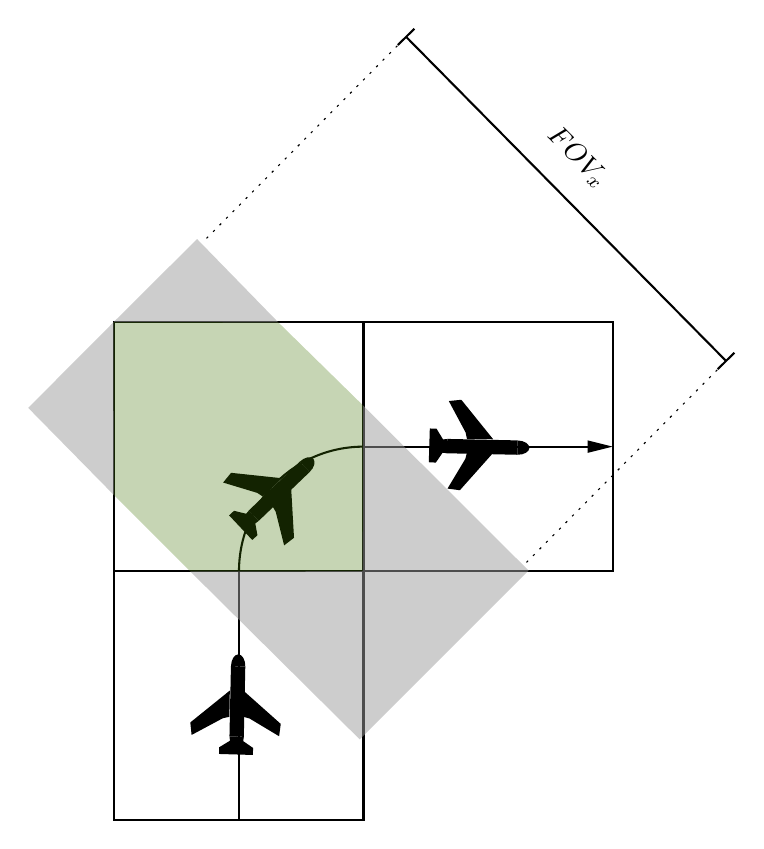
\begin{tikzpicture}[x=0.75pt,y=0.75pt,yscale=-1,xscale=1]
	%uncomment if require: \path (0,483); %set diagram left start at 0, and has height of 483
	
	%Shape: Square [id:dp7554025064162504] 
	\draw  [line width=0.75]  (184.88,300) -- (304.88,300) -- (304.88,420) -- (184.88,420) -- cycle ;
	%Shape: Square [id:dp029527299824832154] 
	\draw  [line width=0.75]  (184.88,180) -- (304.88,180) -- (304.88,300) -- (184.88,300) -- cycle ;
	%Shape: Square [id:dp05898723469860556] 
	\draw  [line width=0.75]  (304.88,180) -- (424.88,180) -- (424.88,300) -- (304.88,300) -- cycle ;
	%Straight Lines [id:da2896157813713012] 
	\draw [line width=0.75]    (244.88,300) -- (244.88,420) ;
	%Straight Lines [id:da6458424182642684] 
	\draw [line width=0.75]    (422.88,240) -- (304.88,240) ;
	\draw [shift={(424.88,240)}, rotate = 180] [fill={rgb, 255:red, 0; green, 0; blue, 0 }  ][line width=0.08]  [draw opacity=0] (12,-3) -- (0,0) -- (12,3) -- cycle    ;
	%Shape: Arc [id:dp6697923261787817] 
	\draw  [draw opacity=0][line width=0.75]  (244.88,300) .. controls (244.88,266.86) and (271.74,240) .. (304.88,240) -- (304.88,300) -- cycle ; \draw  [line width=0.75]  (244.88,300) .. controls (244.88,266.86) and (271.74,240) .. (304.88,240) ;
	%Shape: Chord [id:dp19722764417953975] 
	\draw  [draw opacity=0][fill={rgb, 255:red, 0; green, 0; blue, 0 }  ,fill opacity=1 ][line width=0.75]  (274.12,247.29) .. controls (276.41,245.09) and (279.34,244.42) .. (280.66,245.79) .. controls (281.97,247.17) and (281.18,250.07) .. (278.88,252.27) -- cycle ;
	%Shape: Rectangle [id:dp7564053950991294] 
	\draw  [draw opacity=0][fill={rgb, 255:red, 0; green, 0; blue, 0 }  ,fill opacity=1 ][line width=0.75]  (278.88,252.27) -- (254.42,275.73) -- (249.64,270.73) -- (274.1,247.27) -- cycle ;
	%Shape: Chord [id:dp8544272377140341] 
	\draw  [draw opacity=0][fill={rgb, 255:red, 0; green, 0; blue, 0 }  ,fill opacity=1 ][line width=0.75]  (254.42,275.73) .. controls (254.42,275.73) and (254.42,275.73) .. (254.42,275.73) .. controls (252.12,277.93) and (249.2,278.6) .. (247.88,277.22) .. controls (246.57,275.85) and (247.36,272.95) .. (249.66,270.75) -- cycle ;
	%Shape: Boxed Polygon [id:dp4243302902770245] 
	\draw  [draw opacity=0][fill={rgb, 255:red, 0; green, 0; blue, 0 }  ,fill opacity=1 ][line width=0.75]  (266.64,287.56) -- (262.59,271.38) -- (261.02,268.73) -- (270.02,260.03) -- (271.39,283.91) -- cycle ;
	%Shape: Boxed Polygon [id:dp6815588587808861] 
	\draw  [draw opacity=0][fill={rgb, 255:red, 0; green, 0; blue, 0 }  ,fill opacity=1 ][line width=0.75]  (237.24,257.3) -- (253.63,262.26) -- (256.31,264) -- (265.4,255.2) -- (241.08,252.61) -- cycle ;
	%Shape: Boxed Polygon [id:dp4894660411365015] 
	\draw  [draw opacity=0][fill={rgb, 255:red, 0; green, 0; blue, 0 }  ,fill opacity=1 ][line width=0.75]  (253.78,282.71) -- (251.27,284.96) -- (240.12,273.11) -- (242.5,270.91) -- (252.04,273.24) -- cycle ;
	
	%Shape: Boxed Line [id:dp4808926265834552] 
	\draw  [dash pattern={on 0.84pt off 2.51pt}]  (229.24,139.64) -- (325.41,42.57) ;
	%Straight Lines [id:da17659301005268957] 
	\draw [line width=0.75]    (325.41,42.57) -- (479.55,198.71) ;
	\draw [shift={(479.55,198.71)}, rotate = 225.37] [color={rgb, 255:red, 0; green, 0; blue, 0 }  ][line width=0.75]    (0,5.59) -- (0,-5.59)   ;
	\draw [shift={(325.41,42.57)}, rotate = 225.37] [color={rgb, 255:red, 0; green, 0; blue, 0 }  ][line width=0.75]    (0,5.59) -- (0,-5.59)   ;
	%Shape: Boxed Line [id:dp01374331482035851] 
	\draw  [dash pattern={on 0.84pt off 2.51pt}]  (383.38,295.78) -- (479.55,198.71) ;
	%Shape: Chord [id:dp9231747485755666] 
	\draw  [draw opacity=0][fill={rgb, 255:red, 0; green, 0; blue, 0 }  ,fill opacity=1 ][line width=0.75]  (241.03,345.76) .. controls (241.03,345.76) and (241.03,345.76) .. (241.03,345.76) .. controls (241.1,342.58) and (242.69,340.03) .. (244.6,340.08) .. controls (246.5,340.12) and (247.99,342.73) .. (247.92,345.91) -- cycle ;
	%Shape: Rectangle [id:dp34380596609036296] 
	\draw  [draw opacity=0][fill={rgb, 255:red, 0; green, 0; blue, 0 }  ,fill opacity=1 ][line width=0.75]  (247.92,345.91) -- (247.21,379.79) -- (240.29,379.64) -- (241,345.76) -- cycle ;
	%Shape: Chord [id:dp3433894979507466] 
	\draw  [draw opacity=0][fill={rgb, 255:red, 0; green, 0; blue, 0 }  ,fill opacity=1 ][line width=0.75]  (247.21,379.8) .. controls (247.21,379.8) and (247.21,379.8) .. (247.21,379.8) .. controls (247.21,379.8) and (247.21,379.8) .. (247.21,379.8) .. controls (247.14,382.98) and (245.55,385.52) .. (243.65,385.48) .. controls (241.74,385.44) and (240.26,382.82) .. (240.32,379.64) -- cycle ;
	%Shape: Boxed Polygon [id:dp08898175934962804] 
	\draw  [draw opacity=0][fill={rgb, 255:red, 0; green, 0; blue, 0 }  ,fill opacity=1 ][line width=0.75]  (264.22,379.52) -- (249.92,370.95) -- (246.93,370.18) -- (247.14,357.67) -- (265,373.58) -- cycle ;
	%Shape: Boxed Polygon [id:dp8735831522150785] 
	\draw  [draw opacity=0][fill={rgb, 255:red, 0; green, 0; blue, 0 }  ,fill opacity=1 ][line width=0.75]  (222.04,378.91) -- (237.13,370.83) -- (240.25,370.17) -- (240.46,357.52) -- (221.43,372.88) -- cycle ;
	%Shape: Boxed Polygon [id:dp35625726838667515] 
	\draw  [draw opacity=0][fill={rgb, 255:red, 0; green, 0; blue, 0 }  ,fill opacity=1 ][line width=0.75]  (251.7,385.19) -- (251.51,388.55) -- (235.25,388.06) -- (235.37,384.82) -- (243.77,379.72) -- cycle ;
	
	%Shape: Chord [id:dp34828845330166835] 
	\draw  [draw opacity=0][fill={rgb, 255:red, 0; green, 0; blue, 0 }  ,fill opacity=1 ][line width=0.75]  (379.12,237.02) .. controls (379.12,237.02) and (379.12,237.02) .. (379.12,237.02) .. controls (382.3,237.09) and (384.85,238.69) .. (384.8,240.59) .. controls (384.76,242.49) and (382.15,243.98) .. (378.97,243.91) -- cycle ;
	%Shape: Rectangle [id:dp8474408050833497] 
	\draw  [draw opacity=0][fill={rgb, 255:red, 0; green, 0; blue, 0 }  ,fill opacity=1 ][line width=0.75]  (378.97,243.91) -- (345.09,243.2) -- (345.24,236.28) -- (379.12,236.99) -- cycle ;
	%Shape: Chord [id:dp5085353869793547] 
	\draw  [draw opacity=0][fill={rgb, 255:red, 0; green, 0; blue, 0 }  ,fill opacity=1 ][line width=0.75]  (345.09,243.2) .. controls (345.09,243.2) and (345.09,243.2) .. (345.09,243.2) .. controls (341.9,243.14) and (339.36,241.54) .. (339.4,239.64) .. controls (339.44,237.74) and (342.06,236.25) .. (345.24,236.31) -- cycle ;
	%Shape: Boxed Polygon [id:dp8833099273000848] 
	\draw  [draw opacity=0][fill={rgb, 255:red, 0; green, 0; blue, 0 }  ,fill opacity=1 ][line width=0.75]  (345.36,260.21) -- (353.93,245.91) -- (354.7,242.92) -- (367.21,243.13) -- (351.3,260.99) -- cycle ;
	%Shape: Boxed Polygon [id:dp25055803366441176] 
	\draw  [draw opacity=0][fill={rgb, 255:red, 0; green, 0; blue, 0 }  ,fill opacity=1 ][line width=0.75]  (345.97,218.03) -- (354.05,233.12) -- (354.71,236.24) -- (367.36,236.45) -- (352,217.42) -- cycle ;
	%Shape: Boxed Polygon [id:dp7889546658783853] 
	\draw  [draw opacity=0][fill={rgb, 255:red, 0; green, 0; blue, 0 }  ,fill opacity=1 ][line width=0.75]  (339.7,247.69) -- (336.33,247.5) -- (336.82,231.24) -- (340.06,231.37) -- (345.16,239.76) -- cycle ;
	
	%Shape: Polygon [id:ds23159985077498058] 
	\draw  [draw opacity=0][fill={rgb, 255:red, 155; green, 155; blue, 155 }  ,fill opacity=0.5 ] (304.48,300) -- (304.6,220.1) -- (384.38,299.67) -- (303.03,381.02) -- (221.4,300.1) -- cycle ;
	%Shape: Polygon [id:ds5721792230643707] 
	\draw  [draw opacity=0][fill={rgb, 255:red, 155; green, 155; blue, 155 }  ,fill opacity=0.5 ] (224.69,139.98) -- (263.8,180.1) -- (184.48,180) -- (143.34,221.33) -- (184.6,263.3) -- (184.48,180) -- cycle ;
	%Shape: Polygon [id:ds6510638071272044] 
	\draw  [draw opacity=0][fill={rgb, 255:red, 65; green, 117; blue, 5 }  ,fill opacity=0.3 ] (263.8,180.1) -- (304.6,220.1) -- (304.48,300) -- (221.4,300.1) -- (184.6,263.3) -- (184.48,180) -- cycle ;
	
	
	% Text Node
	\draw (399.45,82.4) node [anchor=north west][inner sep=0.75pt]  [rotate=-45]  {$FOV_{x}$};
	
	
\end{tikzpicture}
	\caption{Figure showing required FOV to ensure no corner cutting on a square discretisation}
	\label{fig:corner_cutting_01}
\end{figure}

\begin{figure}[h!]
	\centering
	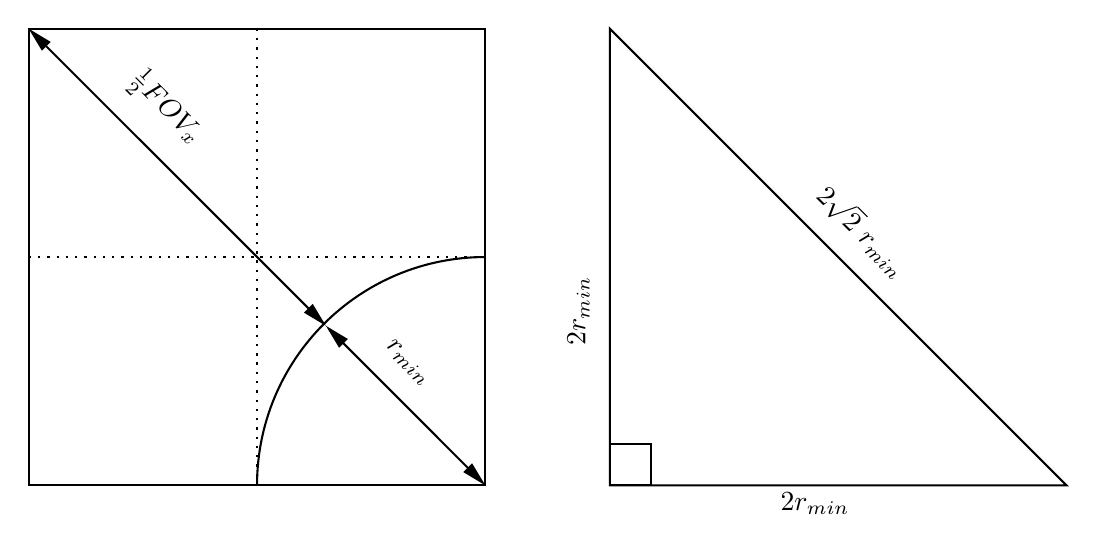
\begin{tikzpicture}[x=0.75pt,y=0.75pt,yscale=-1,xscale=1]
		%uncomment if require: \path (0,464); %set diagram left start at 0, and has height of 464
		
		%Shape: Square [id:dp21273854123077562] 
		\draw  [line width=0.75]  (59,80) -- (279,80) -- (279,300) -- (59,300) -- cycle ;
		%Straight Lines [id:da03805299191386524] 
		\draw [line width=0.75]  [dash pattern={on 0.84pt off 2.51pt}]  (169,80) -- (169,300) ;
		%Straight Lines [id:da4291514540511687] 
		\draw [line width=0.75]  [dash pattern={on 0.84pt off 2.51pt}]  (59,190) -- (279,190) ;
		%Shape: Arc [id:dp32305088211851984] 
		\draw  [draw opacity=0][line width=0.75]  (169,300) .. controls (169,239.25) and (218.25,190) .. (279,190) -- (279,300) -- cycle ; \draw  [line width=0.75]  (169,300) .. controls (169,239.25) and (218.25,190) .. (279,190) ;
		%Straight Lines [id:da34774498940242626] 
		\draw [line width=0.75]    (60.41,81.41) -- (200.78,221.74) ;
		\draw [shift={(202.2,223.15)}, rotate = 224.99] [fill={rgb, 255:red, 0; green, 0; blue, 0 }  ][line width=0.08]  [draw opacity=0] (12,-3) -- (0,0) -- (12,3) -- cycle    ;
		\draw [shift={(59,80)}, rotate = 44.99] [fill={rgb, 255:red, 0; green, 0; blue, 0 }  ][line width=0.08]  [draw opacity=0] (12,-3) -- (0,0) -- (12,3) -- cycle    ;
		%Straight Lines [id:da24453213307250365] 
		\draw [line width=0.75]    (203.61,224.56) -- (277.59,298.59) ;
		\draw [shift={(279,300)}, rotate = 225.02] [fill={rgb, 255:red, 0; green, 0; blue, 0 }  ][line width=0.08]  [draw opacity=0] (12,-3) -- (0,0) -- (12,3) -- cycle    ;
		\draw [shift={(202.2,223.15)}, rotate = 45.02] [fill={rgb, 255:red, 0; green, 0; blue, 0 }  ][line width=0.08]  [draw opacity=0] (12,-3) -- (0,0) -- (12,3) -- cycle    ;
		%Shape: Right Triangle [id:dp960720423813475] 
		\draw  [line width=0.75]  (339,80) -- (559,300) -- (339,300) -- cycle ;
		%Shape: Square [id:dp6932539999111038] 
		\draw  [line width=0.75]  (359,300) -- (339,300) -- (339,280) -- (359,280) -- cycle ;
		
		% Text Node
		\draw (115,95) node [anchor=north west][inner sep=0.75pt]  [rotate=-45]  {$\frac{1}{2}FOV_{x}$};
		% Text Node
		\draw (235,227.1) node [anchor=north west][inner sep=0.75pt]  [rotate=-45]  {$r_{min}$};
		% Text Node
		\draw (420,302.4) node [anchor=north west][inner sep=0.75pt]    {$2r_{min}$};
		% Text Node
		\draw (317.4,234) node [anchor=north west][inner sep=0.75pt]  [rotate=-270]  {$2r_{min}$};
		% Text Node
		\draw (446.39,150.99) node [anchor=north west][inner sep=0.75pt]  [rotate=-45]  {$2\sqrt{2} \ r_{min}$};
		
		
	\end{tikzpicture}
	\caption{Diagram showing the dimensions necessary to calculate FOV on a square discretisation.}
	\label{fig:corner_cutting_02}
\end{figure}

\begin{equation}
	\label{eqn:r_min}
	\begin{aligned}
		r_{min} = \frac{v^2}{g\tan{(\theta_{max}})}
	\end{aligned}
\end{equation}

\begin{equation}
	\label{eqn:fovx from r_min}
	\begin{aligned}
		\frac{FOV_x}{2} &= 2\sqrt{2}r_{min}-r_{min} &\\
		FOV_x &= r_{min}(4\sqrt{2}-2) &
	\end{aligned}
\end{equation}

\begin{equation}
	\label{eqn:AR}
	\begin{aligned}
		A.R. &= \frac{w_{len}}{h_{len}} &\\
	\end{aligned}
\end{equation}

\begin{equation}
	\label{eqn:fovy from fovx}
	\begin{aligned}
		FOV_y &= \frac{FOV_x}{A.R.}
	\end{aligned}
\end{equation}

\noindent Referring back to Equation \ref{eqn:fov_x}, one can calculate the minimum allowable height for this velocity using the following: 

\begin{equation}
	\label{eqn:H_min}
	\begin{aligned}
		H_{min} = \frac{FOV_x \times f}{w_{len}}
	\end{aligned}
\end{equation}

\noindent Section \ref{sec:ER-ED} chooses the maximum allowable \ac{gsd} of 4cm/px for this application. From this, a maximum allowable height can be calculated using Equation \ref{eqn:max_height_calculation}. Now, any height between $H_{min}$ and $H_{max}$ can be selected. The \ac{fov} at that height can then be calculated using Equations \ref{eqn:fov_x} and \ref{eqn:fov_y}. 

Equation \ref{eqn:fovx from r_min} can then be reformulated to calculate the appropriate size of a square discretisation for this \ac{fov}. The radius in the equation is now the maximum allowable radius for this discretisation. This should be equal to or more than the minimum turning radius, which is limited by the velocity.

\begin{equation}
	\label{eqn:}
	\begin{aligned}
		r_{max} &= \frac{FOV_x}{4\sqrt{2}-2} &\\
		l &= 2r_{max}
	\end{aligned}
\end{equation}

Equation \ref{} can also be reformulated to calculate the minimum required bank angle to turn within this square discretisation at the chosen velocity. It is then the decision of the operator what bank angle to use for the turns. It can be anywhere between this $\theta_{min}$ and $\theta_{max}$. The minimum is limited by the square discretisation, which is ultimately limited by the \ac{gsd}. The maximum is the mechanical limit of the \ac{uav} itself.
\chapter{Refuelling Protocol}
\label{chp:refuelling}


%%%%%%%%%%%%%%%%%%%%%%%%%%%%%%%%%%%%%%%%%%%%%%%%%%%%%%%%%%%%%%%%%%%%%%%
\section{Background}


\chapter{Results}
\label{chp:Results}


%%%%%%%%%%%%%%%%%%%%%%%%%%%%%%%%%%%%%%%%%%%%%%%%%%%%%%%%%%%%%%%%%%%%%%%



\chapter{Conclusions and Future Work}
\label{chp:Concl}

%==== Appendices ====================================================
\appendix
\appendixpage\relax

\chapter{Discrete Element Method Theory}
\label{chp:DEM-Theory}

\section{Ball elements}
\label{sec:Ball-elems}

\begin{figure}
   \centering
   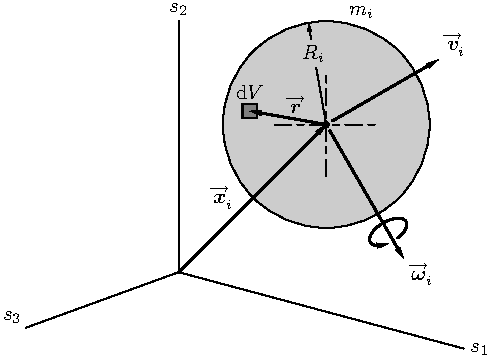
\includegraphics{figs/DEM-Def-Ball}
   \caption{Ball Element Parameters}
   \label{fig:BallDef}
\end{figure}


\subsection{Ball mass and inertia parameters}

Consider a volume element $\mathrm{d}V$ with respect to a static base $S$ of
an arbitrary solid body with  density $\rho$. The mass of the body is
obtained by integrating over the volume of the body,
\begin{equation}
    m = \int\limits_{\mathrm{body}} \rho\, \mathrm{d}V
    \label{eq:BMass-dif}
\end{equation}

In figure~\ref{fig:BallDef}, a ball with radius $R_{i}$ and uniform density
$\rho_i$ is depicted. The mass of the ball is after integration of
equation~\eqref{eq:BMass-dif}
\begin{equation}
    m_i = \tfrac{4}{3} \pi \rho_i\, R_i^3 .
    \label{eq:BMass}
\end{equation}


%----------------------------------------------------------------------------
\endinput

%\include{contents/App-2}
%\include{contents/App-3}

%==== Bibliography acro's & Index ===================================
\backmatter

\bibliography{backmatter/USbib-sample}

\end{document}
